\documentclass
[
a4paper,
ngerman,
oneside,
openright,                    % Kap.beginn immer rechts! (fkt. nur bei report, nicht bei article)
11pt,                         % ersatzweise 12pt, wenn mehr Seiten entstehen sollen
table
]
{report}

%%%%%%%%%%%%%%%%%%%%%%%%%%%%%%%%%%%%%%%%%%%%%%%%%%%%%%%%%%%%%%%%%%%%%%%%%%%%%%
%
% Vorlage für eine Studien- oder Diplomarbeit für den Fachbereich Informatik
% der Universität Karlsruhe (TH)
%
% Autor:   Tilo Gockel
% Version: 0.920
% Datum:   12. Mai 2010
%
% Kontakt: Hochschule Aschaffenburg,
% Tilo Gockel (Dr.-Ing.), Forschungsreferat
%
% info@formbuch.de
% http://www.formbuch.de
%
% Anmerkungen
%
% 1.) article-Style, statt report-Style
%
% Soll statt des report-Styles der article-Style genutzt werden,
% so müssen chapters durch sections, sections durch subsection usw. ersetzt
% werden. Weiterhin kann ein Kapitelbeginn auf der rechten Seite dann nicht
% mehr durch openright eingestellt werden, nur noch durch jeweilige
% \cleardoublepage -Befehle (vgl. unten).
%
%
% 2.) Lizenz
%
% Das Template darf angepasst, verändert, erweitert und auch kommerziell vertrieben werden. 
% Die einzige Auflage ist, dass die Quelle des Templates in den Literaturquellen genannt 
% und im Text als Quelle referenziert wird. Hierzu ist dem Text ein kurzer Satz beizufügen, 
% und am Ende ist die Quelle einzufügen:
% Einzufügende Textzeile (Fußnote):
% Der vorliegende Text ist auf Basis des Latex-Templates zu [1] erstellt.
% Einzufügende zugehörige Quelle:
% [1] T. \mbox{Gockel}. Form der wissenschaftlichen Ausarbeitung. Springer-Verlag, Heidelberg, 2008. 
% Begleitende Materialien unter 
% \url$<http://wwwiaim.ira.uka.de/form-der-wissenschaftlichen-ausarbeitung>$.
% Weiterhin ist es sinnvoll, bei der Weitergabe des Templates die Latex-Quellen und die PDF-Datei
% nicht zu trennen.
%
%
% 3.) Versionsnummern der verwendeten Programme (alles unter Windows)
%
% (im Regelfall werden neuere Versionen aber eher von Vorteil sein)
%
%     Miktex 2.8
%     http://www.miktex.org
%
%     TexnicCenter Version 1.0 Stable Release Candidate 1
%     http://www.texniccenter.org
%
%     Texaide 4.0a
%     http://www.dessci.com/en/products/texaide
%
%     Adobe Acrobat Prof. 7.0
%     http://www.adobe.com/de/
%
%     Ghostscript 8.14, Ghostview 4.6
%     http://pages.cs.wisc.edu/~ghost
%
%     MS Office 2002, 2007 ...
%     http://office.microsoft.com/de-de/default.aspx
%
%     Adobe Photoshop CS4
%     http://www.adobe.com/de/products/photoshop/family/
%
%     Gnuplot 4.2
%     http://www.gnuplot.info
%   
%     PrettyPrinter a2ps
%     http://www.gnu.org/software/a2ps
%
%     Text-Ersetzungswerkzeug grep, unter Windows
%     http://gnuwin32.sourceforge.net/packages/grep.htm
%
%
%%%%%%%%%%%%%%%%%%%%%%%%%%%%%%%%%%%%%%%%%%%%%%%%%%%%%%%%%%%%%%%%%%%%%%%%%%%%%%



\usepackage[utf8]{inputenc}   % Zeichensatz, ermöglicht die direkte Eingabe von Umlauten im Editor
\usepackage[pdftex]{graphicx} % Einbindung von Grafiken (pdf, png, jpg)
\usepackage{float}            % bietet Option [H] für bombenfestes Verankern
\usepackage[ngerman]{babel}   % Silbentrennung nach der neuen deutschen Rechtschreibung, z.B.: Sys-tem
\usepackage{amstext}          % für Klartext via \text{} in Formeln
\usepackage{amsfonts}         % für komplexere Formeln (Mengensymbole ...)
\usepackage{amssymb}          % für komplexere Formeln (Mengensymbole ...)
\usepackage{bm}               % bold math, für \bm{}
\usepackage{enumerate}        % verbessert Aufzählungen
\usepackage[bottom]{footmisc} % Fussnoten am Seitenende
\usepackage{array}            % für Tabellen: bindet tabular-Umgebung ein
%\usepackage{algorithm}        % für Algorithmen
%\usepackage{algorithmic}      % für Algorithmen
\usepackage{ntheorem}
\usepackage{theorem}
\usepackage{pdfpages}         % für die Einbindung kompletter pdf-*Seiten*
\usepackage{parskip}          % zw. Absätzen: eine knappe Leerzeile statt hängender Einzüge
\usepackage[right]{eurosym}   % Eurosymbol
%\usepackage{xcolor}           % farbiger Text
%\usepackage{colortbl}
\usepackage{xcolor}
%\usepackage[hyphens]{url}     % für \url{http://www}, Option hyp erlaubt auch Umbruch nach "-"
\usepackage{makeidx}          % Package zur Indexerstellung
\usepackage{multicol}         % zur Indexerstellung in zwei Spalten
\usepackage[numbers, square]{natbib}   % Für \setlength{\bibsep}{3mm}; square macht eckige Klammern
\usepackage[T1]{fontenc}
\usepackage{hyperref}
%\usepackage{tabularx}
\usepackage{caption}
\usepackage[printonlyused]{acronym}
\usepackage{listings}
\usepackage{chngcntr}

\counterwithout{figure}{chapter}
\counterwithout{table}{chapter}

\captionsetup[table]{skip=10pt}

\NeedsTeXFormat{LaTeX2e}            % Unklar, gehoeren aber zusammen:
\ProvidesPackage{hyperref}          % http://janeden.net/eigene-dokumentklassen
\hypersetup{
  pdftex=false,
  colorlinks=true,
  breaklinks=true,
  linkcolor=black,
  menucolor=black,
  urlcolor=black,
  citecolor=black
}


%\usepackage[cmex10]{amsmath}  % für erw. Formeloptionen, Option [] zur Vermeidung von Type3-Fonts
%\usepackage{mathcomp}         %\tcmu \tcohm \tccelsius.. im Mathemodus, nichtkursiv; problematisch!
%\usepackage{textcomp}         % für \textdegree , \textcelsius , macht aber manchmal auch Probleme!


%\usepackage[plainpages=false, hypertexnames=false]{hyperref}
                               % hyperref statt \url geht, verträgt sich allerdings nicht mit den 
                               % eingefügten / veränderten Seitenzahlen ... (die stimmen dann nicht mehr)
                                


\definecolor{darkred}{rgb}{0.7,0.0,0.0}
\definecolor{dunkelgrau}{rgb}{0.8,0.8,0.8}
\definecolor{hellgrau}{rgb}{0.92,0.92,0.92}
\definecolor{fgcgray}{rgb}{0.4, 0.4, 0.4}
\definecolor{bgctitle}{rgb}{0.5, 0.5, 0.5}
\definecolor{fgctitle}{rgb}{0.95, 0.95, 0.95}
\definecolor{lightgreen}{RGB}{219, 249, 189}
\definecolor{lightred}{RGB}{255, 204, 203}

%\definecolor{lightgray}{rgb}{.9,.9,.9}
%\definecolor{darkgray}{rgb}{.4,.4,.4}
%\definecolor{purple}{rgb}{0.65, 0.12, 0.82}
%
%\definecolor{js-keywords}{RGB}{243, 38, 77}
%\definecolor{js-strings}{RGB}{211, 214, 95}
%\definecolor{js-comments}{RGB}{117, 113, 94}

\renewcommand{\lstlistlistingname}{Quellcodeverzeichnis}
\renewcommand{\lstlistingname}{Quellcode}

\lstdefinelanguage{JavaScript}{
  keywords={typeof, new, true, false, catch, function, return, null, catch, switch, var, if, in, while, do, else, case, break},
  %keywordstyle=\color{js-keywords}\bfseries,
  ndkeywords={class, export, boolean, throw, implements, import, this},
  %ndkeywordstyle=\color{darkgray}\bfseries,
  %identifierstyle=\color{black},
  sensitive=false,
  comment=[l]{//},
  morecomment=[s]{/*}{*/},
  %commentstyle=\color{js-comments}\ttfamily,
  %stringstyle=\color{js-strings}\ttfamily,
  morestring=[b]',
  morestring=[b]"
}

\lstset{
    language=JavaScript,
    basicstyle=\small\sffamily,
    numbers=left,
    frame=single,
    columns=fullflexible,
    showstringspaces=false,
    captionpos=b,
    xleftmargin=2em,
    framexleftmargin=2.0em,
    numberbychapter=false
}

\lstset{literate=%
{Ö}{{\"O}}1 
{Ä}{{\"A}}1 
{Ü}{{\"U}}1 
{ß}{{\ss}}2 
{ü}{{\"u}}1 
{ä}{{\"a}}1 
{ö}{{\"o}}1
}



\sloppy                       % großzügiger Zeilenumbruch 
                              % -> keine rechts rausragenden Zeilen mehr


%%%%%%%%%%%%%%%%%%%%%%%%%%%%%%%%%%%%%%%%%%%%%%%%%%%%%%%%%%%%%%%%%%%%%%%%%%%%%%
%
% Index-Erstellung
%
% Anmerkung: für die Indexerstellung muss auch die TeXnicCenter-IDE angepasst 
% werden:
% 1.) Projekt / Eigenschaften / verwendet MakeIndex [x] 
% 2.) Ausgabe / Ausgabeprofil definieren
%
\makeindex % erstelle einen Index bzw. ein Sachverzeichnis)
%
% Wenn kein Index gewünscht ist: einfach \makeindex auskommentieren
%
%%%%%%%%%%%%%%%%%%%%%%%%%%%%%%%%%%%%%%%%%%%%%%%%%%%%%%%%%%%%%%%%%%%%%%%%%%%%%%



%%%%%%%%%%%%%%%%%%%%%%%%%%%%%%%%%%%%%%%%%%%%%%%%%%%%%%%%%%%%%%%%%%%%%%%%%%%%%%
%
% Literaturverzeichnis mit BibTeX
%
\bibliographystyle{alphadin} 
\setlength{\bibsep}{3mm}                  % Abstände im Litverzeichnis
%
% Anmerkung: das Dokument enthält _zwei_ Literaturverzeichnisse
% 1.) Ein auf Basis von bibliografie.bib mit BibTeX erstelltes Verzeichnis
% 2.) Ein einfach getipptes Verzeichnis: Literatur.tex
%
% -> das nicht gewünschte einfach auskommentieren
%
%%%%%%%%%%%%%%%%%%%%%%%%%%%%%%%%%%%%%%%%%%%%%%%%%%%%%%%%%%%%%%%%%%%%%%%%%%%%%%



%%%%%%%%%%%%%%%%%%%%%%%%%%%%%%%%%%%%%%%%%%%%%%%%%%%%%%%%%%%%%%%%%%%%%%%%%%%%%%
%
% Größenanpassungen
%
\setlength{\unitlength}{1cm}
\setlength{\oddsidemargin}{0.3cm}
\setlength{\evensidemargin}{0.3cm}
\setlength{\textwidth}{15.5cm}
\setlength{\topmargin}{-1.2cm}
\setlength{\textheight}{23cm}
\columnsep 0.5cm
%
%%%%%%%%%%%%%%%%%%%%%%%%%%%%%%%%%%%%%%%%%%%%%%%%%%%%%%%%%%%%%%%%%%%%%%%%%%%%%%



%%%%%%%%%%%%%%%%%%%%%%%%%%%%%%%%%%%%%%%%%%%%%%%%%%%%%%%%%%%%%%%%%%%%%%%%%%%%%%
%
% Beispiel für die Anpassung des Satzspiegels und 
% die Verwendung von Schnittmarken (momentan ausgeschaltet)
% Im Beispiel: Anpassung des Drucks auf Taschenbuchformat 
%
% Obacht: für Tests hiermit (Probeausdrucke...): 
% stets im Adobe Acrobat im Druckdialog die Seitenanpassung *abschalten*!
% sonst stimmen die Maße nicht!
% 
%
%\usepackage[total={90mm,144mm},centering]{geometry}
%\geometry{papersize={120mm,190mm}} 
%\usepackage[a4,cam,center]{crop}
%\crop[]
%
% Schnittmarken und Satzspiegel - Ende
%
%%%%%%%%%%%%%%%%%%%%%%%%%%%%%%%%%%%%%%%%%%%%%%%%%%%%%%%%%%%%%%%%%%%%%%%%%%%%%%



%%%%%%%%%%%%%%%%%%%%%%%%%%%%%%%%%%%%%%%%%%%%%%%%%%%%%%%%%%%%%%%%%%%%%%%%%%%%%%
%
% Abkürzungsliste, Liste explizit vorgegebener Abk.
%
% Anmerkung: für Wörter mit Umlauten
% muss das Paket \usepackage[T1]{fontenc} eingebunden werden --
% in der vorliegenden Version funktionieren *keine* Umlaute!!
% 
\hyphenation{Da-tei-grö-ßen-be-schränk-ung Au-then-ti-fi-zier-ung Ent-wick-ler-apps Ent-wick-ler-app Hash-funk-tion-en Ver-schlüs-sel-ungs-algo-rith-mus} 
%
%%%%%%%%%%%%%%%%%%%%%%%%%%%%%%%%%%%%%%%%%%%%%%%%%%%%%%%%%%%%%%%%%%%%%%%%%%%%%%


\begin{document}
\def\cpp{C{}\texttt{++}} % \cpp is shortcut now for: print C++ nicely

\pagestyle{empty}
\begin{titlepage}
\begin{figure}
  \begin{center}
    \hbox to \hsize{%
      \begin{tabular}[m]{c}
        
\includegraphics[width=2.5cm]{resources/Bilder_Allgemein/HTW_Logo_rgb.jpg}
      \end{tabular}
      \hfill%
      \begin{tabular}[m]{c}
        Hochschule für Technik und Wirtschaft Berlin (HTW)\\
        Fachbereich 4 - Wirtschaftswissenschaften II \\
      \end{tabular}
    }
  \end{center}
\end{figure}

\begin{center}
\rule{0pt}{0pt}
\vfill
\vfill
\vfill
\vfill

\begin{huge}
Bachelor Thesis:\\[0.75ex]
Untersuchung zu Möglichkeiten des Dateimanagements unter Verwendung verschiedener Cloudanbieter\\[0.75ex]
\end{huge}

\vfill
\vfill

Bachelorarbeit\\ von\\

\vspace*{.5cm}
Markus Paeschke\\
\vspace{.5cm}
03. Juni 2013 -- 13. August 2013 \\

\vfill
\vfill
\vfill
\vfill

\begin{tabular}{rl}
Prüfungsvorsitzender: & Prof. Dr. Albrecht Fortenbacher\\

Betreuer: & Prof. Dr. Christin Schmidt\\
& Prof. Dr. Albrecht Fortenbacher
\end{tabular}
\end{center}
\end{titlepage}

\newpage
\text{ }
\vspace{13.5cm}

Ich möchte mich bei Prof. Dr. Christin Schmidt für die Betreuung und Begleitung, während der Erstellung dieser Arbeit, bedanken, genauso wie bei Prof. Dr. Albrecht Fortenbacher, für die Hilfestellungen und nützlichen Ratschläge.

Ein besonderer Dank geht an Nora Mudrack, Daniel Ghioreanu und Andreas Buff, die mir nicht nur bei der Bachelorarbeit behilflich waren, sondern mich mein ganzes Studium über unterstützt haben und mir immer wieder Kraft und Motivation zum weitermachen gegeben haben. Danke dafür.

Weiterhin danke ich Grit Schneider, Angela Mehnert und Toralf Kampe für das Korrekturlesen und die hilfreichen Ratschläge bei der Erstellung dieser Arbeit.
\newpage
\text{ }
\vspace{13.5cm}


Markus Paeschke\\
Trachtenbrodtstr. 32\\
10409 Berlin\\

Hiermit versichere ich, dass ich die von mir vorgelegte Arbeit selbstständig verfasst habe, dass ich die verwendeten Quellen, Internet-Quellen und Hilfsmittel vollständig angegeben habe und dass ich die Stellen der Arbeit -- einschließlich Tabellen, Karten und Abbildungen~--, die anderen Werken oder dem Internet im Wortlaut oder dem Sinn nach entnommen sind, auf jeden Fall unter Angabe der Quelle als Entlehnung kenntlich gemacht habe.\\

Berlin, den \today\\
\medskip
\medskip

(Unterschrift)\\
\underline{~~~~~~~~~~~~~~~~~~~~~~~~~~~~~~~~~~~~~~~~}\\
Markus Paeschke\\

\newpage


\pagestyle{plain}
\pagenumbering{roman}
\setcounter{page}{3}

\tableofcontents
\cleardoublepage


\phantomsection
\addcontentsline{toc}{chapter}{Abkürzungsverzeichnis}
\renewcommand\refname{Abkürzungsverzeichnis}
\section*{Abkürzungsverzeichnis}
\begin{acronym}[HTTPS] % längste Abkürzung steht in eckigen Klammern
    \setlength{\itemsep}{-\parsep} % geringerer Zeilenabstand
    
    % A
    \acro{AES}{Advanced Encription Standard}
    \acro{AGB}{Allgemeine Geschäftsbedingungen}
        \acrodefplural{AGB}[AGBs]{Allgemeine Geschäftsbedingungen}
    \acro{API}{Application Programming Interface}
        \acrodefplural{API}[APIs]{Application Programming Interfaces}
    \acro{App}{Application}
        \acrodefplural{App}[Apps]{Applications}
    % B
    % C
    \acro{CRM}{Customer-Relationship-Management}
    \acro{CSS}{Cascading Style Sheets}
    % D
    \acro{DES}{Data Encryption Standard}
    \acro{DOM}{Document Object Model}
    % E
    \acro{E/A}{Ein-/Ausgabe}
    % F
    % G
    \acro{GB}{Gigabyte}
    \acro{GHz}{Gigahertz}
    \acro{GUI}{Graphical User Interface}
    % H
    \acro{HTML}{Hypertext Markup Language}
    \acro{HTTP}{Hypertext Transfer Protocol}
    \acro{HTTPS}{Hypertext Transfer Protocol Secure}
    % I
    \acro{IaaS}{Infrastructure as a Service}
    \acro{I/O}{Input/Output}
    % J
    \acro{JIT}{Just-In-Time}
    \acro{JSON}{JavaScript Object Notation}
    \acro{JVM}{Java Virtual Machine}
    % K
    \acro{KB}{Kilobyte}
    % L
    % M
    \acro{MB}{Megabyte}
    \acro{MD5}{Message-Digest Algorithm 5}
    \acro{MIME}{Multipurpose Internet Mail Extensions}
    \acro{MIT}{Massachusetts Institute of Technology}
    \acro{MVC}{Model View Controller}
    % N
    \acro{NIST}{National Institute of Standards and Technology}
    \acro{NSA}{National Security Agency}
    % O
    % P
    \acro{PaaS}{Platform as a Service}
    % Q
    % R
    \acro{RAID}{Redundant Array of Inexpensive Disks}
    \acro{REST}{Representational State Transfer}
    \acro{upm}{Umdrehungen pro Minute}
    \acro{RSA}{Rivest, Shamir und Adleman}
    % S
    \acro{SaaS}{Software as a Service}
    \acro{SATA}{Serial Advanced Technology Attachment}
    \acro{Sass}{Syntactically Awesome Stylesheets}
    \acro{SHA}{Secure-Hash-Algorithm}
    \acro{SQL}{Structured Query Language}
    \acro{SSH}{Secure Shell}
    \acro{SSL}{Secure Socket Layer-Technologie}
    % T
    % U
    \acro{URI}{Uniform Resource Identifier}
        \acrodefplural{URI}[URIs]{Uniform Resource Identifiers}
    \acro{URL}{Uniform Resource Locator}
        \acrodefplural{URL}[URLs]{Uniform Resource Locators}
    % V
    % W
    % X
    \acro{XML}{Extensible Markup Language}
    % Y
    % Z
\end{acronym}

\listoffigures
\protect \addcontentsline{toc}{chapter}{Abbildungsverzeichnis}
\cleardoublepage

\listoftables
\protect \addcontentsline{toc}{chapter}{Tabellenverzeichnis}
\cleardoublepage

\lstlistoflistings
\protect \addcontentsline{toc}{chapter}{Quellcodeverzeichnis}
\cleardoublepage

\pagenumbering{arabic}
\setcounter{page}{1}

\chapter{Einleitung}
\label{einleitung}

\section{Motivation}
\label{motivation}
Clouddienste erfreuen sich in den letzten Jahren einer rasant wachsenden Beliebtheit.
Der Umsatz in Deutschland wird, laut einer Prognose von Bitkom, im Jahr 2013 um 47\% gegenüber dem Vorjahr ansteigen und liegt damit bei 7,8 Millarden Euro\cite[vgl.][Seite 2]{bitkom13}.
Ebenfalls geht aus dieser Prognose hervor, dass sich auch in den kommenden Jahren ein ähnlich starkes Wachstum fortsetzt.
So ist es nicht verwunderlich, dass immer mehr Anwendungen einen Upload der Daten in die Cloud ermöglichen oder gar komplett die Datenspeicherung in die Cloud verlagern.

Von einem einfachen Datenbackup wie bei Dropbox\footnote{\url{http://www.dropbox.com}} oder Google Drive\footnote{\url{http://drive.google.com}}, zum Musikstreaming wie Spotify\footnote{\url{http://www.spotify.com}}, bis hin zum kollaborativen Arbeiten in den Google Docs\footnote{\url{http://docs.google.com}}, die Anwendungsgebiete sind dabei vielfältig und wachsen stetig.
Google hat mit seinem Chromium OS\footnote{\url{http://www.chromium.org/chromium-os}} darüber hinaus ein cloudfähiges Betriebssystem auf den Markt gebracht.
Dieses setzt ausschließlich auf Cloudanwendungen und ist ohne einen Internetanschluss nicht nutzbar.

Jedoch sind viele Benutzer skeptisch bei der Verwendung von Clouddiensten.
So geht aus einer Studie von Pierre Audoin Consultants hervor, dass 76\% der Befragten Bedenken in Bezug auf Sicherheit und Datenschutz bei der Verwendung von Clouddiensten haben \cite[vgl.][Seite 23]{pier13}.
Bereits im Jahr 2010 gaben 72\% der deutschen Teilnehmer in einer Studie von Fujitsu an, dass sie befürchten, dass der Staat ihre Daten in der Cloud einsehen kann\cite[vgl.][Seite 05]{fuji13}.
Darüber hinaus besteht jederzeit die Gefahr eines Datenverlustes.
Die möglichen Szenarien sind dabei vielfältig.
Die Anbieter, bei denen die Daten gespeichert werden, können ihren Dienst einstellen, wie es beispielsweise bei Megaupload im Jahr 2012 der Fall war\cite[vgl.][]{mega12}.
Auch denkbar ist, dass sich Hacker Zugriff auf das System verschaffen und somit an die Daten der Nutzer gelangen.

An diesem Punkt setzt die Bachelorarbeit an.
Sie soll aufzeigen, welche Möglichkeiten sich für einen Benutzer bei der Verwendung von verschiedenen Cloudanbietern ergeben und wie in diesem Zusammenhang eine höhere Datensicherheit gewährleistet werden kann.
Dazu werden Probleme bestehender Cloudservices aufgezeigt und Lösungskonzepte für selbige erarbeitet.

\section{Zielsetzung}
\label{zielsetzung}
Ziel dieser Arbeit ist es, einen Prototypen, im folgenden CloudGrid genannt, zu entwickeln, der einerseits eine größere Datensicherheit für Dateien in der Cloud gewährleistet, andererseits den Speicherplatz von Cloudanbietern zusammenfasst und diesen dadurch vergrößert.
Die Datensicherheit soll durch mehrere Methoden erhöht werden.
Zum einen sollen die Daten in den gebündelten Clouds redundant gespeichert werden, was den Vorteil hat, das ein Service ausfallen und der Benutzer trotzdem über alle Daten verfügen kann.
Weiterhin werden Dateien komprimiert, zerteilt und danach auf verschiedenen Cloudanbietern gespeichert.
Das hat zur Folge, dass Daten nie vollständig bei einem Anbieter gespeichert werden und dadurch für Dritte nur bedingt brauchbar sind.
Zugleich werden diese noch komprimiert, sodass mehr Speicherplatz zur Verfügung steht.
Darüber hinaus werden alle Dateien verschlüsselt.
Der Inhalt der Daten soll somit geschützt werden.

CloudGrid soll als reine Desktopanwendung umgesetzt werden und damit komplett auf einen Serverdienst verzichten.
Dies hat den Vorteil, dass sich der Benutzer nicht bei einem weiteren Service anmelden und seine Daten erneut an eine weitere Institution schicken muss.
Dabei soll im Rahmen dieser Arbeit lediglich die Datenverwaltung mit einem Client zugelassen werden.
Eine Synchronisierung über mehrere Clients erhöht die Komplexität und wird für eine etwaige spätere Version vorgesehen.

\section{Aufbau der Arbeit}
\label{aufbau}
Zu Beginn werden Grundlagen zu Clouddiensten, Sicherheit und Dateihandling aufgezeigt.
Anschließend werden die Anforderungen an den zu entwickelnden Prototypen definiert, sowie deren Besonderheiten und Möglichkeiten dargestellt.
Darauf basierend wird die Architektur des Systems dargestellt und abschließend die konkrete Umsetzung erläutert.
Zudem wird die Funktionsweise des Prototypen demonstriert und auf Defizite hingewiesen.
Abschließend wird eine Zusammenfassung über die gewonnenen Kenntnisse und ein Ausblick auf Erweiterungsmöglichkeiten dieser Thematik 
erörtert.

% Chapter 1 - Grundlagen
\chapter{Grundlagen}

\section{Clouddienste}
Das Thema Cloud-Computing ist momentan allgegenwärtig in der Informatik.
Dennoch gibt es keine standardisierte Definition, was die "`Cloud"' ist.
Das Wort "`Cloud"' oder im deutschen "`Wolke"' weist jedoch auf zwei wichtige Konzepte hin, nämlich Virtualisierung und Skalierbarkeit\cite[vgl.][Seite 35]{hoell11}.
Bei der Virtualisierung werden Computerressourcen transparent zusammengefasst beziehungsweise aufgeteilt.
Dadurch wird eine beliebige Sicht auf die Infrastruktur geschaffen, wodurch keine systembedingten Abhängigkeiten für eine Anwendung entstehen\cite[vgl.][Seite 2]{baun10}.

Der zweite wichtige Aspekt, die Skalierbarkeit, ermöglicht es, zusätzliche Ressourcen ohne großen Aufwand in das System zu integrieren, sei es um Hardware nachzurüsten oder bestehende Systeme zusammen zu fassen.
Das hat den Vorteil, dass ein Unternehmen nicht mehr in diese investieren und selbst verwalten muss.
Es kann sich auf die Umsetzung seiner Geschäftsidee konzentrieren und bei wachsenden Anforderungen Ressourcen flexibel vom Provider beziehen\cite[vgl.][Seite 2]{baun10}.

Als großer Kritikpunkt lassen sich hingegen die Sicherheitsbedenken aufführen.
Dadurch, dass die Anwendungslogik an eine externe Firma ausgelagert wird, verliert das Unternehmen die Kontrolle über seine Daten.
Zudem muss es sich auf die Sicherheitsmaßnahmen der Anbieter verlassen und hat keinen Einfluss auf selbige.
Besonders bei sensiblen Daten, wie Krankenakten von Patienten oder Kundendaten einer Bank, spielen Sicherheitsaspekte eine übergeordnete Rolle, wodurch unter Umständen von der Verwendung von Cloud-Computing abgeraten werden muss.
Auch die Verfügbarkeit und Performance von Ressourcen in einer Cloud geben Grund zur Kritik.
Sollte ein Service für mehrere Stunden nicht verfügbar sein, so kann ein erheblicher wirtschaftlicher Schaden für die betroffene Firma entstehen.
Zudem existieren momentan keine Standards bei der Implementierung von Ressourcen, womit ein schneller Wechsel des Anbieters in der Regel nicht einfach möglich ist\cite[vgl.][Seite 3]{baun10}.

Je nach Anwendungsfall muss ein Unternehmen sich daher detailliert überlegen, ob es Cloud-Computing verwenden möchte und welche Form und welcher Anbieter dabei seinen Ansprüchen genügt.

Neben der Auslagerung von Anwendungslogiken gibt es mehrere Dienste die vorgefertigte Lösungen anbieten.
So streamen Spotify\footnote{\url{http://www.spotify.com}} oder Deezer\footnote{\url{http://www.deezer.com}} Musik, Youtube\footnote{\url{http://www.youtube.de}} streamt Videos, Google Docs\footnote{\url{https://docs.google.com/}} bietet eine komplette Office Suite zum kollaborativen Arbeiten an und sogar Bildbearbeitung ist mit Diensten wie dem Photoshop Express Editor\footnote{\url{http://www.photoshop.com/tools/expresseditor}} möglich.
Die Vorteile für den Benutzer liegen dabei auf der Hand.
Er kann mobil und über verschiedene Geräte hinweg seine Daten abrufen und bearbeiten, ohne dabei auf zusätzliche Hardware wie USB-Sticks oder DVDs zurückgreifen zu müssen.
Darüber hinaus muss sich der Anwender nicht mehr manuell um die Aktualisierung seiner Daten auf verschiedene Geräte kümmern.
Beispielsweise bearbeitet er ein Foto in der Cloud, speichert dieses dort und kann es später von einem anderen Rechner herunterladen.
Dadurch, dass sich der Anbieter des Clouddienstes um ein sinnvolles Datenbackup kümmern muss, beispielsweise durch redundante Datenhaltung auf mehreren Servern, wird für den Benutzer eine Ausfallsicherheit gewährleistet.
Sollte der Rechner defekt sein, gehen die Daten nicht verloren, sondern sind weiterhin auf dem Server verfügbar.

Zudem kann die Architektur von Clouddiensten aus zwei Perspektiven betrachtet werden.
Einerseits aus organisatorischer Sicht und andererseits aus technischer Sicht\cite[vgl.][Seite 25]{baun10}.
Zu den erstgenannten zählen die "`Private Cloud"', die "`Public Cloud"' und die "`Hybrid Cloud"'\cite[vgl.][Seite 25]{baun10}.
Clouddienste, die aus technischen Sicht betrachtet werden, können in "`\ac{IaaS}"', "`\ac{PaaS}"' und "`\ac{SaaS} eingeteilt werden\cite[vgl.][Seite 25]{baun10}.

\subsection{Clouddienste aus organisatorischer Sicht}
Bei der organisatorischen Betrachtung von Clouddiensten, werden Benutzer und Anbieter strukturell voneinander getrennt.
Der Benutzer verwendet dabei einen Dienst, welcher vom Anbieter offeriert wird.
Beide Einheiten können dem selben Unternehmen angehören, werden jedoch separate betrachtet.

\subsubsection{Private Cloud}
Unter "`Private Cloud"' versteht man eine Cloud, bei der sowohl die Benutzer als auch der Anbieter derselben organisatorischen Einheit angehören\cite[vgl.][Seite 25 f.]{baun10}.
Es ist also ein geschlossenes Netzwerk, wie beispielsweise ein firmeninternes Intranet, welches den Benutzern exklusive Ressourcen zur Verfügung stellt\cite[vgl.][Seite 40]{hoell11}.
Hauptgrund für die Verwendung von "`Private Clouds"' sind Sicherheitsaspekte.
Gerade bei sensiblen Daten ist diese Art der Cloud von großem Vorteil, da sich dadurch viele Sicherheitsprobleme beseitigen lassen.
So bleibt die Kontrolle über die Daten bei der Organisation selbst und wird nicht an Dritte weitergeben\cite[vgl.][Seite 26]{baun10}.
Außerdem können einzelne Ressourcen kontrollierter an Benutzer weitergegeben werden.
Ein Mitarbeiter erhält so zwar Zugang zu seinem eigenen Dienstplan, jedoch nicht zu dem seiner Kollegen, wohingegen der Geschäftsführer Zugriff auf alle Dienstpläne hat.
Auch Hardwareressourcen können flexibel skaliert und entsprechend der aktuellen Situation angepasst werden.

Jedoch muss die Verwaltung und Wartung der Cloud, sowohl soft- als auch hardwareseitig, von der Organisation selbst übernommen werden.
Dieser Aspekt ist aus unternehmerischer Sicht kostenintensiver und daher möglicherweise unattraktiver.
Besonders da diese, je nach Umfang, von einem oder mehreren Administratoren gepflegt werden muss.

\subsubsection{Public Cloud}
Eine "`Public Cloud"' kann als ein am Markt angebotener Clouddienste angesehen werden\cite[vgl.][Seite 38]{hoell11}.
Es sind also Cloud-Angebote, bei denen der Anbieter und die potenziellen Benutzer nicht zu ein- und derselben organisatorischen Einheit gezählt werden\cite[vgl.][Seite 25]{baun10}.
Meist sind jene Anbieter gemeint, wenn von der "`Cloud"' gesprochen wird.
Die Ressourcen solcher Dienste werden meist von vielen Nutzern gleichzeitig geteilt, welche nur durch die Virtualisierung als eigene Umgebung für den einzelnen Benutzer erscheinen.
Viele Dienstleister bieten darüber hinaus ein Web-Portal oder gar eine \ac{API} zum Interagieren mit dem Dienst an.
Diese sind für den Betreiber leicht skalierbar, sodass weitere Hardwareressourcen jederzeit eingebunden werden können.
Besonders bei wachsenden Anforderungen an das System ist dieser Aspekt essenziell.
Auf Seiten des Nutzers lässt sich dieses Prinzip nur schwer anwenden.
"`Eine Anpassung an spezifische Anwenderanforderungen ist üblicherweise nur sehr eingeschränkt möglich/erwünscht bzw. steht den Skalierungs- und Effizienzinteressen des Betreibers gegenüber"'\cite[Seite 39]{hoell11}.

Eine übliche Bezahlmethode ist "'Pay-per-Use"', das bedeutet je nach benutzten Ressourcen fallen mehr oder weniger hohe Kosten an, sowie die "`Flatrate"', für die der Nutzer einen festen Betrag bezahlt, wobei er einen vordefinierten Umfang der Ressourcen zur Verfügung gestellt bekommt.
Ein prominenter Vertreter für "`Pay-per-User"' ist Amazon EC2\footnote{\url{http://aws.amazon.com/de/ec2}}, wohingegen beispielsweise Dropbox\footnote{\url{https://www.dropbox.com/business}} oder Spotifiy\footnote{\url{https://www.spotify.com/de}} auf ein Flaterate-Model setzen.

Gerade im Gegensatz zu "`Private Clouds"' ergeben sich bei den "`Public Clouds"' zahlreiche Bedenken.
So muss für jedes System "`hinsichtlich Compliance, Sicherheit, Verfügbarkeit, aber auch Performance"'\cite[Seite 40]{hoell11}. detailliert geprüft werden, ob eine "`Public Cloud"' den Anforderungen gerecht wird.
Durch den Verlust der, im Vergleich zu den "`Private Clouds"', absoluten Kontrolle über die Daten des Benutzers, müssen beim Verstoß gegen vertraglich vereinbarte Regelungen, diese erst juristisch durchgesetzt werden\cite[vgl.][Seite 40]{hoell11}.
Besonders der zeitliche Aspekt von Gerichtsverfahren birgt ein großes Risiko für Unternehmen.

\subsubsection{Hybrid Cloud}
"`Hybrid Clouds"' sind eine Mischform aus "`Public Clouds"' und "`Private Clouds"'.
Hierbei wird eine "`Private Cloud"' auf organisationseigenen Ressourcen betrieben, jedoch werden zusätzlich Services herkömmlicher Datenverarbeitungslösungen mittels \acp{API} von "`Public Cloud"' Anbietern eingebunden.
Somit können konkrete Anforderungen an ein System für das jeweilige Unternehmen angepasst werden.
Etwaige Sicherheitsvorgaben können eingehalten werden und gleichzeitig Skalierungseffekte genutzt werden\cite[vgl.][Seite 42]{hoell11}.
Durch Virtualisierung wird auch bei "`Hybrid Clouds"' dem Benutzer ein geschlossenes System dargestellt, sodass dieser weder einen Unterschied noch einen Übergang zwischen den einzelnen Clouds bemerkt\cite[vgl.][Seite 11]{hoell11}.

Als Nachteil kann eine erhöhte Komplexität bei der Integration solcher Systeme aufgeführt werden.
Eine nahtlose und für den Benutzer transparente Implementierung muss sorgfältig geplant und von den entsprechenden Administratoren und Entwicklern eingebunden werden.
Zudem muss detailliert geprüft werden, welche Komponenten in die "`Public Clouds"' auszulagern sind, damit die Nachteile selbiger nicht das Gesamtsystem beeinträchtigen.

\subsection{Clouddienste aus technischer Sicht}
Bei der technischen Betrachtung der Clouddienste wird eine abstrahiert Sicht auf Hard- und Software geboten.
Der Anbieter kümmert sich um die Wartung und Pflege der Ressourcen, wohingegen der Kunde virtualisierte Ressourcen angeboten bekommt.

\subsubsection{Infrastructure as a Service}
Einem Benutzer wird bei der Verwendung der \ac{IaaS}-Schicht eine abstrahierte Sicht auf die Hardware, also unter anderem auf ein bestehendes Netzwerk, einen Server und deren räumliche und klimatische Bedingungen oder auch nur auf Massenspeichermedien, geboten\cite[vgl.][Seite 47]{hoell11}.
Dabei wird dem Kunden meist eine Teilmenge der eigentlichen Ressourcen zur Verfügung gestellt.
"`Man könnte IaaS auch als eine im Wesentlichen durch Einsatz von Software abstrahierte und virtualisierte Rechenzentrumsressource auffassen"'\cite[Seite 47]{hoell11}.
Das bedeutet, dass sich meist mehrere Kunden ein und dieselbe Ressource teilen, welche lediglich auf Softwareebene virtualisiert wird.
Besonders in Hinsicht auf die Skalierbarkeit der Ressourcen ist das ein erheblicher Vorteil.

Als Beispiel für solche Services kann man virtuelle Server von Hostingprovidern oder auch Dienste wie Amazon EC2 und Dropbox nennen.
Letztere bieten darüber hinaus noch Schnittstellen zur Kommunikation mit den Diensten an, wohin gegen virtuelle Server meist über einen \ac{SSH} Zugang verfügen.

\subsubsection{Platform as a Service}
Die \ac{PaaS}-Schicht baut auf der \ac{IaaS}-Schicht auf und bietet dem Benutzer Anwendungen, Datenbanken oder Webservices, mit denen er arbeiten kann.
Oftmals wird diese auch als \frqq Middleware\flqq\ bezeichnet\cite[vgl.][Seite 47]{hoell11}.
In der Praxis richtet sich dieser Service meist an Entwickler.
Der Vorteil gegenüber \ac{IaaS} ist ein verminderter Wartungsaufwand.
Das bedeutet, dass es nicht mehr notwendig ist Software auf einem virtuellen Server zu aktualisieren oder eine Firewall auf selbigem zu konfigurieren.
Ähnlich wie bei \ac{IaaS} ist auch dieser Service leicht skalierbar und kann flexibel an die Bedürfnisse eines Unternehmens angepasst werden.

Prominente Vertreter für diese Art von Services sind Microsoft Azure\footnote{\url{http://www.windowsazure.com/de-de}} und Google App Engine\footnote{\url{https://cloud.google.com/products}}.
Beide verfügen über ein ähnliches Angebot und ermöglichen eine stundenweise Nutzung und Bezahlung.

\subsubsection{Software as a Service}
Zur \ac{SaaS}-Schicht gehören Anwendungen in der Cloud, die direkt an den Endkunden adressiert sind\cite[vgl.][Seite 35]{baun10}.
Dabei wird die Software direkt angeboten, ohne dass sich der Kunde um die Wartung weiterer Ressourcen kümmern muss.
Alle zur Ausführung erforderlichen Ressourcen werden durch den Anbieter gestellt und gepflegt.
"`Den Anspruch als Cloud-Computing-Service erfüllt es allerdings nur dann, wenn das Angebot massiv skalierbar, mehrmandantenfähig und elastisch flexibel ist"'\cite[Seite 47]{hoell11}.

Diese Art von Service ist die derzeit am häufigsten angebotene und diskutierte Form Cloudservices\cite[vgl.][Seite 47]{hoell11}.
Beispiele für diese Art des Services sind Google Maps, Google Docs oder das \ac{CRM} von salesforce\footnote{\url{https://www.salesforce.com/de/form/sem/landing/sales-cloud.jsp}}.
%
%\subsection{Zusammenfassung}
%Cloudservices erfreuen sich großer Beliebtheit.
%Aktuell ist diese ein häufig diskutiertes Thema und immer mehr Anbieter präsentieren sich auf dem Markt.
%Jedoch muss ein Unternehmen genau abwägen welche Services es nutzen möchte und welche optimal zu dem eigenen Produkt passen.
%\ac{SaaS}-Services richten sich dabei oftmals an Endverbraucher und sind für Firmen ehr uninteressant, jedoch können diese gerade beim kollaborativen Arbeiten einen großen Mehrwert bieten.
%In der Praxis erweisen sich \ac{PaaS} und \ac{IaaS} Services als sinnvolle Lösungen für einzelne Unternehmungen.
%Gerade durch eine preiswerte Nutzung und attraktiven Bezahlmodellen wie Pay-per-use sind "`Public Clouds"' oftmals eine gute Wahl.
%Jedoch sollten für jeden Anwendungsfall detailliert die Vor- und Nachteile abgewogen werden.
%Besonders im Bereich Datensicherheit.
%Unternehmen welche mit sensiblen Daten arbeiten, sollten daher lieber in eine "`Private Cloud"' investieren oder, insofern es zum Konzept des Produktes passt, in eine "`Hybrid Cloud"', welche Teilaskpekte in einen "`Public Cloud"' Service auslagert.
%
\section{RAID Systeme}
Bei einem \ac{RAID} System werden mehrere Festplatten zu einer großen virtuellen Festplatte zusammengefasst\cite[vgl.][Seite 279 f.]{mandl13}.
Daraus resultiert, dass mindestens zwei Festplatten für den Betrieb eines \ac{RAID}-Systems erforderlich sind.
Solch ein System aus mehreren Festplatten wird auch vom Betriebssystem als eine einzige logische Festplatte angesehen\cite[vgl.][Seite 279 f.]{mandl13}.
Daten, welche in einem \ac{RAID}-System gespeichert werden sollen, werden je nach verwendetem Verfahren über die physikalischen Festplatten verteilt oder redundant auf mehreren Platten gleichzeitig gespeichert\cite[vgl.][Seite 279 f.]{mandl13}.
Insgesamt existieren sieben \ac{RAID}-Systeme, welche von 0 bis 6 durchnummeriert sind\cite[vgl.][Seite 428 ff.]{hert03}.
Auch Kombinationen aus mehreren Verfahren sind möglich.
In Anbetracht dessen, dass nur \ac{RAID}-0 und \ac{RAID}-1 für diese Arbeit relevant sind, da \ac{RAID}-2 bis \ac{RAID}-6 die Datenspeicherung von der Speicherung der Prüfinformationen trennen, werden diese fünf Verfahren nicht näher erläutert\cite[vgl.][Seite 430 ff.]{hert03}.
Für eine komplette Übersicht aller Verfahren sei auf die Literatur \cite{mandl13} verwiesen.

\subsection{RAID-0}
Ein \ac{RAID}-0-System verbindet mehrere physikalische Festplatten zu einer einzigen virtualisierten Einheit.
Dabei werden sogenannte Stripes auf den Platten angelegt, welche üblicherweise über Größen von 32, 64 und 128 \ac{KB} verfügen.
Man spricht hierbei auch von der Striping-Granularität\cite[vgl.][Seite 281 f.]{mandl13}.
Eine Datei wird demnach zerteilt und auf alle Festplatten verteilt.
Der Vorteil dieses Verfahrens liegt in dem hohen \ac{E/A}-Durchsatz\cite[vgl.][Seite 281 f.]{mandl13}.
Jedoch ist dieses System nicht ausfallsicher, da keine Redundanz gespeichert wird.
Im Sinne der Definition ist das \ac{RAID}-0-System daher kein echtes \ac{RAID}-System\cite[vgl.][Seite 281 f.]{mandl13}.
Abbildung \ref{fig-raid-0} zeigt dieses Verfahren auf.

\begin{figure}[H]
  \centering
  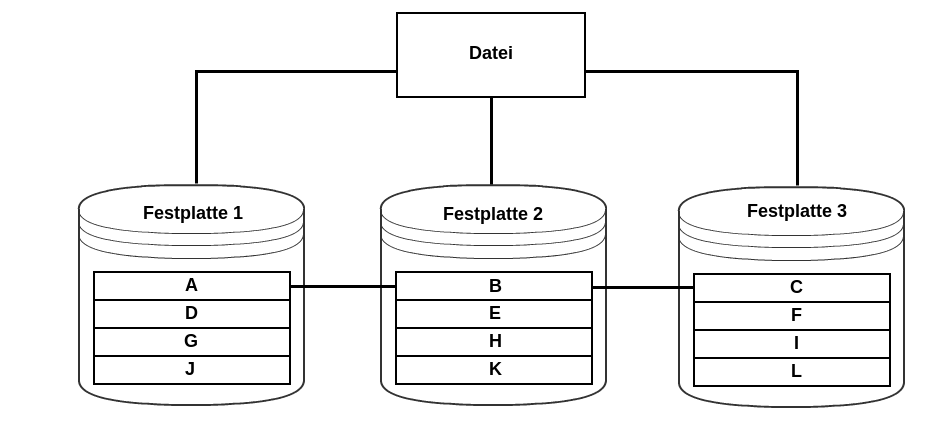
\includegraphics[scale=0.3]{resources/Bilder_Kapitel_2/RAID-0.png}
  \caption[Verteilung der Teilstücke einer Datei unter Verwendung von RAID-0]{Verteilung der Teilstücke einer Datei unter Verwendung von RAID-0 (In Anlehnung an \cite[Seite 279]{mandl08})}
  \label{fig-raid-0}
\end{figure}

Auf jede der drei Festplatten, in der Abbildung durch Festplatte 1, Festplatte 2 und Festplatte 3 dargestellt, werden verschiedene Teilstücke einer Datei, mit den Buchstaben A bis L dargestellt, gespeichert.
Daraus geht hervor, dass die Datei in mehrere Einzelstücke unterteilt und nicht redundant gespeichert wird.
Sollte eine Festplatte ausfallen, ist die gesamte Datei ungültig und nicht mehr brauchbar.

\subsection{RAID-1}
Bei einem \ac{RAID}-1-System werden alle Daten redundant auf die unterschiedlichen physikalischen Laufwerke gespeichert.
Sollte der \ac{RAID}-Verbund beispielsweise aus vier Festplatten bestehen, so wird eine Datei x auf allen vier Festplatten als Kopie abgelegt.
Das garantiert eine größere Ausfallsicherheit, da im Falle eines Defekts einer Festplatte, die Daten noch auf weiteren Platten verfügbar sind.
Dabei ist zu beachten, dass die Gesamtgröße der virtuellen Festplatte durch die kleinste verwendeten Platte festgelegt wird\cite[vgl.][Seite 281]{mandl13}.
Die Anzahl der Festplatten kann beliebig gewählt werden.
Je mehr Festplatten, desto größer die Ausfallsicherheit, wobei ein Benutzer immer den Kosten-Nutzen-Faktor abwägen muss.
Das bedeutet, sowohl die Kosten für eine Anschaffung steigen, als auch die Schreibzugriffe.
Ab einer gewissen Anzahl von Festplatten sinkt jedoch die Chance, dass alle zur gleichen Zeit ausfallen, auf einen vernachlässigbaren Prozentsatz.
Der Nachteil bei diesem Verfahren liegt im Schreibvorgang.
Dadurch, dass auf mehreren logischen Festplatten dieselbe Datei gespeichert werden muss, nimmt dies unter Umständen mehr Zeit in Anspruch als beim Beschreiben einer einzelnen Festplatte.
Jedoch kann je nach Einstellung der Lesevorgang beschleunigt werden, indem einzelne Sektoren der Datei von einzelnen Festplatten gelesen werden und später zusammengeführt werden\cite[vgl.][Seite 429 f.]{hert03}.
Dieses Verfahren wird in Abbildung \ref{fig-raid-1} aufgezeigt.

\begin{figure}[H]
  \centering
  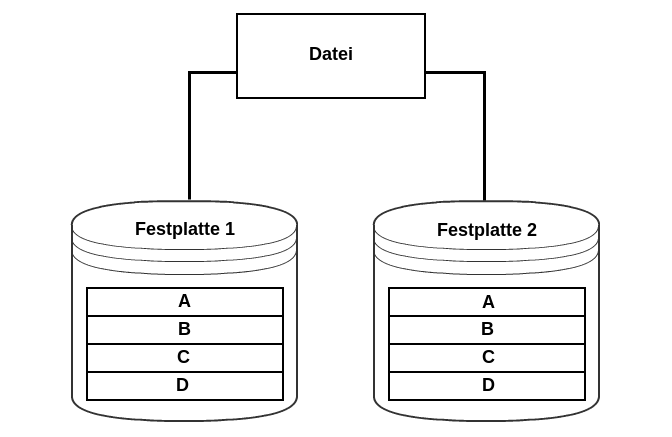
\includegraphics[scale=0.3]{resources/Bilder_Kapitel_2/RAID-1.png}
  \caption[Verteilung der Teilstücke einer Datei unter Verwendung von RAID-1]{Verteilung der Teilstücke einer Datei unter Verwendung von RAID-1 (In Anlehnung an \cite[Seite 280]{mandl08})}
  \label{fig-raid-1}
\end{figure}

Eine Datei wird auf zwei Festplatten, in der Abbildung durch Festplatte 1 und Festplatte 2 gekennzeichnet, gespeichert.
Obwohl zwei Festplatten verwendet werden, erhöht sich die Speicherkapazität nicht, da alle Teilstücke einer Datei, in der Abbildung als A bis D angegeben, gleichermaßen auf beide Festplatten verteilt werden.
Der Vorteil liegt jedoch in der Ausfallsicherheit.
Sollte eine der beiden Festplatten ausfallen, liegt eine Kopie der Datei immer noch auf der zweiten Festplatte, sodass der Benutzer der \ac{RAID}-1-Systems weiterhin Zugriff auf seine Daten hat.
Die defekte Festplatte müsste dann ausgetauscht und die Datei erneut kopiert werden.

\subsection{RAID-1+0}
Das \ac{RAID}-1+0 System, welches auch als \ac{RAID}-10 bezeichnet wird, kombiniert die Vorteile von \ac{RAID}-0 und \ac{RAID}-1-Systemen.
Für dieses Verfahren werden mindestens vier physikalische Festplatten benötigt\cite[vgl.][Seite 282]{mandl13}.
Jeweils 2 Platten werden dann als ein \ac{RAID}-0-Verbund zusammengeschlossen und die zwei daraus resultierenden logischen Festplatten als \ac{RAID}-1-Verbund\cite[vgl.][Seite 282]{mandl13}.
Somit ist eine Ausfallsicherheit gegeben, da Daten redundant gespeichert werden\cite[vgl.][Seite 282]{mandl13}.
Diese Verknüpfung der beiden \ac{RAID}-Systeme wird in Abbildung \ref{fig-raid-10} aufgezeigt.

\begin{figure}[H]
  \centering
  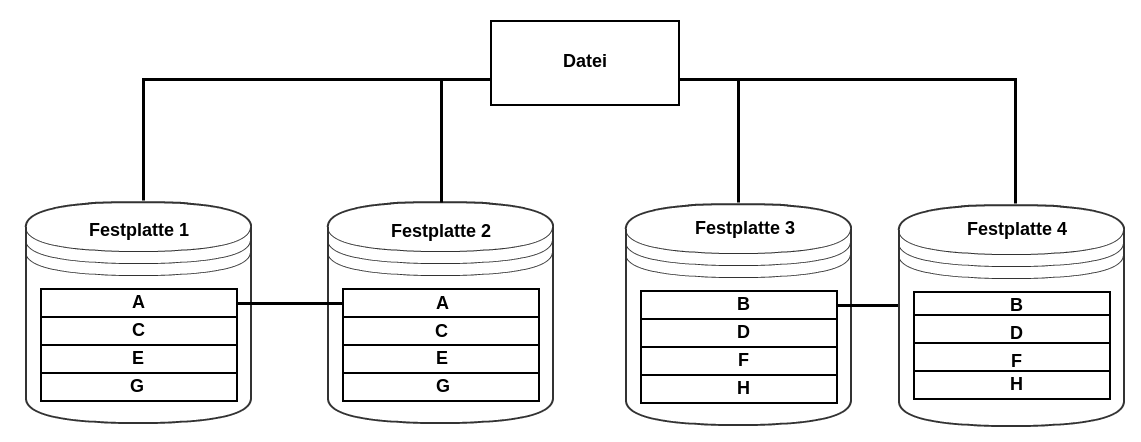
\includegraphics[scale=0.3]{resources/Bilder_Kapitel_2/RAID-10.png}
  \caption[Verteilung der Teilstücke einer Datei unter Verwendung von RAID-1+0]{Verteilung der Teilstücke einer Datei unter Verwendung von RAID-1+0 (In Anlehnung an \cite[Seite 281]{mandl08})}
  \label{fig-raid-10}
\end{figure}

Die Datei wird einerseits, wie bei einem \ac{RAID}-0-System, geteilt und der Speicherplatz somit vergrößert, andererseits werden die Daten auch redundant gespeichert, wie in einem \ac{RAID}-1-System.
Das Prinzip eines \ac{RAID}-1-Systems erkennt man in der Abbildung beispielhaft an Festplatte 2 und Festplatte 3.
Auch hier wird die Datei in Teilstücke von A bis H zerteilt und gespeichert.
Weiterhin kann man die redundante Speicherung eines \ac{RAID}-1-Systems an Festplatte 1 und Festplatte 2 erkennen.
Diese speichern beide dieselben Dateiinformationen, was bedeutet, dass bei einem Ausfall einer dieser Platten die Datei trotzdem verfügbar ist.
Somit sind die Vorteile beider Systeme in einem vereint.
Ein Benutzer vergrößert seinen Speicherplatz und erhält zugleich eine größere Ausfallsicherheit.
%
%   \subsection{Zusammenfassung}
%   \ac{RAID}-Systeme finden besonders bei Systemen mit hohen Datensicherheit oder großen Leistungsansprüchen anwendung.
%   Sollte auf eine hohe Ausfallsicherheit wert gelegt werden so empfiehlt sich das \ac{RAID}-1 System, da es Daten redundant speichert.
%   Wenn hingegen ein schneller Schreib- und Lesezugriff auf Daten gewährleistet werden soll, so sollte ein \ac{RAID}-0 System verwendet werden.
%   \ac{RAID}-1+0 vereint dabei beide Ansprüche, benötigt aber weitaus mehr Hardwareressourcen.
%   Sowohl das \ac{RAID}-0 als auch das \ac{RAID}-1 sind Verfahren, welche für die zu entwickelnde Anwendung in Betracht gezogen werden können.
%

\section{Kryptographie}
\label{kryptographie}
In diesem Abschnitt wird auf kryptographische Grundlagen eingegangen, welche bei der Umsetzung des zu entwickelnden Systems relevant sind.
Dazu werden zuerst Zufallszahlen und deren Besonderheiten aufgezeigt.
Nachfolgend wird ein kurzer Überblick über verschiedene Verschlüsselungsverfahren, sowie deren Vor- und Nachteile herausgearbeitet.
Abschließend werden Hashfunktionen erklärt und ein erweitertes Verfahren zur Nutzung selbiger, welches als Salt bezeichnet wird, erarbeitet.

\subsection{Zufallszahlen}
\label{zufallszahlen}
Zufallszahlen finden in vielen Computerprogrammen Anwendung.
So können zufällige Laufwege von Figuren in einem Computerspiel berechnet, eine Playlist von Musiktiteln zufällig durchlaufen oder Bilder in eine Diashow in einer zufälligen Reihenfolge angezeigt werden\cite[vgl.][Seite 62]{ling02}.
Dabei werden die Zufallszahlen von einem Zufallsgenerator erzeugt.
Jedoch ist der Zufall "`auf Tastendruck"' nicht so leicht zu realisieren\cite[vgl.][Seite 62]{ling02}.
Aus diesem Grund spricht man auch von Pseudozufallsfolgen.

\subsubsection{Pseudozufallsfolgen}
\label{pseudozufallsfolgen}
Das Problem bei Zufallszahlen ist, dass nicht ohne Weiteres ein "`echter Zufall"' erzeugt werden kann\cite[vgl.][Seite 62]{ling02}.
Die Zahlenfolge wird von einem Algorithmus erzeugt, welcher bei gleichem Ausgangswert, auch das gleiche Ergebnis liefert\cite[vgl.][Seite 62]{ling02}.
Daher spricht man in diesem Zusammenhang von "`Pseudozufallsfolgen"'.
Diese reichen in vielen Fällen aus, beispielsweise bei den genannten Anwendungsbeispielen, bieten jedoch für die Kryptographie eine nur unzureichende Sicherheitsmöglichkeit\cite[vgl.][Seite 62]{ling02}.

\subsubsection{Kryptographisch sichere Zufallsfolgen}
\label{sicherzufallsfolgen}
Die kryptographisch sicheren Zufallsfolgen unterscheiden sich von den Pseudozufallsfolgen.
Diese werden immer noch von einem Zufallsgenerator erzeugt und unterliegen auch einem Algorithmus, jedoch sind sie an bestimmte Kriterien gebunden\cite[vgl.][Seite 63 ff.]{ling02}.
"`Demgemäß dürfen Zufallsfolgen mit realistischem Aufwand nicht vorhersagbar sein. Das bedeutet, daß selbst bei Kenntnis des Verfahrens, wie die Zufallsfolge erzeugt wurde, keinerlei Möglichkeit bestehen sollte, dieselbe Folge zu generieren"'\cite[Seite 63]{ling02}.
Dazu werden unterschiedliche Verfahren verwendet.
So können beispielsweise die Systemzeit, ein Mausbewegungsmuster oder Tastatureingaben verwendet werden.
Ferner kann auch auf spezielle Hardware zurück gegriffen werden, welche physikalische Messwerte benutzt um diese in die Generierung mit einfließen zu lassen\cite[vgl.][Seite 63 ff.]{ling02}.

\subsection{Symmetrische Verschlüsselungsverfahren}
\label{symmetrischekrypto}
Ein Verschlüsselungsverfahren wandelt einen Klartext in einen für Menschen nicht lesbaren Text um\cite[vgl.][Seite 15]{ling02}.
Ziel ist es, eine Nachricht von A nach B zu übertragen, ohne das Unbefugte diese lesen können.
Um einen Text zu verschlüsseln, wird ein Schlüssel, oder auch Passphrase, verwendet.
Wenn sowohl zur Chiffrierung, als auch zur Dechiffrierung ein und derselbe Schlüssel verwendet wird, dann spricht man von symmetrischen Verschlüsselungsverfahren\cite[vgl.][Seite 69]{ling02}.
Dieser Schlüssel muss sowohl dem Sender als auch dem Empfänger vorliegen, sodass dieser zuvor ausgetauscht werden muss.
Darin besteht auch das größte Sicherheitsrisiko, da ein Angreifer beispielsweise den Schlüssel beim Übertragen abfangen oder sich als Empfänger tarnen könnte\cite[vgl.][Seite 69]{ling02}.
Um dieses Konzept zu umgehen wurde, 1978 das asymmetrische Verschlüsselungsverfahren RSA, welches nach den Anfangsbuchstaben der Entwickler Rivest, Shamir und Adleman benannt wurde, entwickelt\cite[vgl.][Seite 115]{ling02}.
Dieses verwendet zum Chiffrieren und zum Dechiffrieren einen eigenen Schlüssel.
Es wird auch als Public-Key-Verschlüsselung bezeichnet\cite[vgl.][Seite 110]{ling02}.
Da jedoch letzteres Verfahren im Rahmen dieser Arbeit keine Relevanz hat, wird nur auf symmetrische Verfahren detailliert eingegangen.

\subsubsection{Blockchiffren}
\label{blockchiffren}
Bei dem Blockchiffrenverfahren werden sowohl Klartext als auch der Chiffretext in einzelne Blöcke fester Länge unterteilt, welche in eigenen Vorgängen unabhängig von den anderen Blöcken verschlüsselt beziehungsweise entschlüsselt werden\cite[vgl.][Seite 72]{ling02}.
Dabei kann die Blocklänge, je nach verwendetem Verfahren, variieren\cite[vgl.][Seite 72]{ling02}.
Sollte ein Block nicht die volle Länge besitzen, so wird dieser mit den fehlenden Bits aufgefüllt, was als Padding bezeichnet wird\cite[vgl.][Seite 72]{ling02}.
Die Chiffrierung eines Blocks wird dabei als Runde bezeichnet, sodass ein Verfahren mehrere Runden durchlaufen muss.
Die Anzahl der Runden ist dabei ebenfalls von dem verwendeten Verfahren abhängig.

\subsubsection{DES}
\label{des}
Der \ac{DES} wurde 1974 von IBM veröffentlicht und 1977 zum offiziellen Verschlüsselungsstandard erklärt.
Sowohl die Blocklänge, als auch die Schlüssellänge des \ac{DES} betragen 64 Bit, wobei bei der Schlüssellänge 8 Bit als Prüfsumme verwendet werden und somit real nur 56 Bit zur Verfügung stehen\cite[vgl.][Seite 78]{ling02}.
Somit ergeben sich 2$^{56}$ mögliche Schlüssel, das entspricht 72 Billiarden Schlüsseln\cite[vgl.][Seite 80]{ling02}.
Das größte Sicherheitsrisiko liegt dennoch in der Schlüssellänge.
Hochleistungsrechner oder auch Botnetze können eine solche Schlüssellänge mit Bruteforce-Attacken in wenigen Stunden entschlüsseln\cite[vgl.][Seite 80]{ling02}.
Daher gilt \ac{DES} heutzutage nicht mehr als sicher.
Aus diesem Grund wurde der Triple-\ac{DES} Algorithmus eingeführt.
Selbiger wendet lediglich \ac{DES} drei mal auf eine Nachricht an\cite[vgl.][Seite 82]{ling02}.
Dadurch steigt die Schlüssellänge, je nach Modus, entweder auf 112 Bit bei zwei verschiedenen Schüsseln oder auf 168 Bit bei drei verschiedenen Schlüsseln\cite[vgl.][Seite 82]{ling02}.
Der Aufwand für einen potenziellen Angreifer steigt dabei erheblich, was aus der Verwendung von 2$^{112}$ beziehungsweise 2$^{168}$ möglichen Schlüsseln resultiert\cite[vgl.][Seite 82]{ling02}.
Lediglich die Geschwindigkeit ist der große Nachteil dieses Verfahrens.
Es gibt mehrere Algorithmen, die schneller arbeiten, jedoch als genauso oder sogar sicher als Triple-\ac{DES} gelten.

\subsubsection{AES}
\label{aes}
Im Jahr 2000 wurde der \ac{AES} als Nachfolger von \ac{DES} eingeführt\cite[vgl.][Seite 90]{ling02}.
\ac{AES} verwendet den Rijndael-Algorithmus, der von Joan Daemen und Vincent Rijmen, im Rahmen einer internationalen Ausschreibung zur Einreichung von Vorschlägen für den \ac{AES} im Jahr 1997, entwickelt wurde\cite[vgl.][Seite 89]{ling02}.
Dieser arbeitet mit 128-, 192- oder 256-Bit-Blöcken und mit einer Schlüssellänge von 128, 192 oder 256 Bit\cite[vgl.][Seite 89]{ling02}.
Die Rundenanzahl basiert sowohl auf der Block-, als auch auf der Schlüssellänge.
Bis heute gilt dieses Verfahren als sicher\cite[vgl.][Seite 94]{ling02}.
Für die Beschreibung der detaillierte Funktionsweise von \ac{AES} sei auf die Literatur \cite[Seite 81 ff.]{spitz11} verwiesen.
%TODO mehr?

\subsubsection{Blowfish}
\label{blowfish}
Der Blowfish-Algorithmus wurde im Jahr 1994 von Bruce Schneier veröffentlicht\cite[vgl.][Seite 96]{ling02}.
Er arbeitet wesentlich schneller als \ac{DES} und verwendet ausschließlich einfache Operationen wie Addition und XOR\cite[vgl.][Seite 96]{ling02}.
Die Schlüssellänge hingegen ist variabel und beträgt zwischen 32 und 448 Bit\cite[vgl.][Seite 96]{ling02}.
"`Das Verfahren basiert auf zwei Teilen, einer Schlüsselexpansion, die den bis zu 448 Bit großen Schlüssel in verschiedene Teilschlüssel [...] umwandelt, die zusammen 4168 Bit ergeben. Die eigentliche Chiffrierung wird in einer Funktion F in sechzehn Runden vollzogen. Die einzelnen Runden bestehen aus einer schlüssel- und datenabhängigen Substitution und einer schlüsselabhängigen Permutation"'\cite[Seite 97]{ling02}.
Für die detaillierte Funktionsweise des Blowfishalgorithmus sei auf die Literatur \cite{ling02} verwiesen.
Blowfish ist frei zugänglich und steht damit für kommerzielle und nicht-kommerzielle Anwendungen zur Verfügung.
Bis heute gibt es keine nennenswerten Schwachstellen in der Verschlüsselung\cite[vgl.][Seite 100]{ling02}.

\subsubsection{Twofish}
\label{twofish}
Twofish ist eine Weiterentwicklung des Blowfish-Algorithmus und wurde ebenfalls von Bruce Schneier, von seiner Firma Counterpane Internet Security, veröffentlicht.\cite[vgl.][Seite 100]{ling02}
Das Verfahren war eines von fünf beim Ausscheid zur Bestimmung des Nachfolgers von \ac{DES}\cite[vgl.][Seite 100]{ling02}.
Jedoch unterlag er, genau wie Blowfish, dem Rijndael-Algorithmus in direkten Geschwindigkeitsvergleich.
Genau wie Blowfish ist er frei verfügbar, was ihn sowohl für nicht-kommerzielle als auch für kommerzielle Anwendungen prädestiniert.
Die Schlüssellänge beträgt 128, 192 oder 256 Bit, bei einer Blocklänge von 128 Bit und 16 Runden.
Auch dieser Algorithmus zählt bis heute als sicher\cite[vgl.][Seite 100 f.]{ling02}.
Er wird in Programmen wie TrueCrypt\footnote{http://www.truecrypt.com} oder auch KeePass\footnote{http://www.keepass.com} verwendet.

\subsection{Hashfunktionen}
\label{hashfunktionen}
Hashfunktionen zählen zur symmetrischen Kryptographie.
Sie erzeugen aus einer Nachricht beliebiger Länge eine Prüfsumme, oftmals auch als Hashsumme oder Hashwert bezeichnet, fester Länge, meist 128 oder 160 Bit lang\cite[vgl.][Seite 127]{ling02}.
Im Gegensatz zur Chiffrierung, darf aus einem Hashwert die originale Nachricht nicht wiederhergestellt werden können\cite[vgl.][Seite 127]{ling02}.
Dieses Verfahren nennt man Einweg-Hashfunktionen.
Weiterhin müssen Hashfunktionen kollisionsresistent sein.
Das bedeutet, dass es nahezu unmöglich sein muss, zwei unterschiedliche Nachrichten mit gleichem Hashwerten zu finden\cite[vgl.][Seite 127]{ling02}.
Dies wiederum schließt nicht aus, dass es diese gibt.
Nahezu unmöglich bedeutet dabei, "`dass es weder mit heutigen Computern, noch mit Rechnern aus der nahen Zukunft möglich sein soll, dies in einem sinnvollen Zeitrahmen zu berechnen"'\cite[Seite 11 f.]{schwenk10}.
Hashfunktionen werden eingesetzt, um Manipulationssicherheit zu gewährleisten.
Anschaulich gesprochen bedeutet das, dass im ersten Schritt die Prüfsumme einer Nachricht erstellt wird.
Daraufhin wird die eigentliche Nachricht vom Sender verschickt.
Der Empfänger berechnet beim Empfangen erneut die Prüfsumme und vergleicht diese dann mit der ersten.
Dies setzt voraus, dass der Empfänger die originale Prüfsumme zuvor erhalten hat.
Sollten beide Werte übereinstimmen, kann der Empfänger davon ausgehen, dass die Nachricht nicht verändert wurde.
Wenn die Werte hingegen nicht übereinstimmen, kann die Nachricht als kompromittiert angesehen werden.
Beispiele dafür sind die Prüfsumme in einem TCP/IP Header oder Session-IDs in Webanwendungen\cite[vgl.][Seite 11 ff.]{schwenk10}.

\subsubsection{MD5}
\label{md5}
Das \ac{MD5} Verfahren erzeugt aus einer Nachricht mit beliebiger Länge eine 128 Bit Prüfsumme\cite[vgl.][Seite 130]{ling02}.
Dieses Verfahren wurde 1991 von Ronald L. Rivest am \ac{MIT}, entwickelt\cite[vgl.][]{md5}.
"`Das Verfahren verarbeitet Blöcke mit einer Länge von 512 Bit und generiert einen 128-Bit-Hashwert"'\cite[vgl.][Seite 130]{ling02}.
Jedoch gilt \ac{MD5} als nur bedingt sicher, nachdem 1996 eine Schwachstelle in der Kompressionsfunktion gefunden wurde\cite[vgl.][Seite 132]{ling02}.
Hans Dobbertin zeige daraufhin auf, wie Kollisionen berechnet werden können\cite[vgl.][Seite 132]{ling02}.
Dies widerspricht der Kollisionsresistenz von Hashfunktionen.
In der Praxis wird von der Nutzung abgeraten\cite[vgl.][Seite 132]{ling02}.

\subsubsection{SHA}
\label{sha}
Die Abkürzung SHA steht für Secure-Hash-Algorithmus und wurde 1993 vom \ac{NIST} in Zusammenarbeit mit der \ac{NSA} entwickelt\cite[vgl.][Seite 131]{ling02}.
Mit Hilfe dieses Verfahrens werden 160 Bit lange Prüfsummen erzeugt\cite[vgl.][Seite 131]{ling02}.
Ähnlich wie auch \ac{MD5} gilt der \ac{SHA} als nicht mehr sicher\cite[vgl.][Seite 132]{ling02}.
Daher wurde 2005 die SHA-2-Familie veröffentlicht.
Diese wird in SHA-224, SHA-256, SHA-384 und SHA-512 unterteilt.
Die Nummer steht dabei für die Länge der resultierenden Prüfsumme.
SHA-2 zählt bis heute als sicher.
Jedoch wurde im Jahr 2008 ein internationaler Wettbewerb gestartet, wo der Nachfolger SHA-3 festgelegt werden sollte.
Im Jahr 2012 wurden Guido Bertoni, Joan Daemen, Michaël Peeters und Gilles Van Assche mit dem von ihnen entwickelten Verfahren, namens "`Keccak"', als Sieger bekannt gegeben\footnote{http://www.nist.gov/itl/csd/sha-100212.cfm}.

\subsubsection{Salt}
\label{salt}
Prüfsummen spielen auch bei der Speicherung von Passwörtern eine große Rolle.
So sollten diese immer als eine Prüfsumme p, welche mit einer Einweg-Hashfunktion H erzeugt wurde, gespeichert werden.
Das erschwert einem potentiellen Angreifer die Ermittlung des originalen Passworts x.
Sollte er jedoch Kenntnisse über das verwendete Hashverfahren haben, so kann er mit sogenannten Rainbowtables die Zeit zum Aufspüren von x senken.
Rainbowtables bestehen meist aus einfachen Key-Value-Pairs.
Der Key gibt dabei die unter Verwendung von H resultierende Prüfsumme und der Value das originale Passwort an.
Der Angreifer muss also lediglich p mit den Prüfsummen aus der Rainbowtable vergleichen und kann somit x ermitteln.
Aus diesem Grund wurde die Verwendung eines Salt entwickelt.
Bei diesem Verfahren wird der Aufwand für den Angreifer nochmals erhöht.
Dazu wird neben dem p, eine weitere Prüfsumme s erstellt.
Diese wird als Salt bezeichnet.
In der einfachsten Form wird H(x + s) = p erzeugt.
Daraus resultiert, dass der Angreifer, bevor er p mit seiner Rainbowtable vergleichen kann, eine neue Table unter Verwendung von s erzeugen muss, um diese dann zu durchlaufen.
Bei einem einzelnen Passwort erhöht dieses Verfahren den Aufwand nur geringfügig, jedoch wird bei großen Benutzer-Datenbanken der Aufwand erheblich erhöht.
Voraussetzung dafür ist, dass jeder Benutzer seinen eigenen Salt erhält.
Darüber hinaus gibt es noch Abwandlungen dieses Verfahrens, wo der Salt nicht an das Ende des Passwortes geschrieben wird, sondern geteilt und an den Anfang und das Ende gestellt wird.
Somit wird der Aufwand zum Ermitteln von x erneut vergrößert, jedoch nur solange der Angreifer keine Kenntnis über die Art der Verwendung von s hat.
\section{OAuth}
\label{oautheinleitung}
Wenn ein Benutzer einer Anwendung den Zugriff auf seine Daten erlauben möchte, die von einer weiteren Anwendung verwaltet wird, so kann er Dank des offenen OAuth Protokolls\footnote{\url{http://oauth.net/documentation}}, dieses ohne seine Zugangsdaten preiszugeben.
Dieses Konzept wird besonders bei \acp{API} eingesetzt.
Prominente Beispiele dafür sind Facebook und Twitter.
Diese ermöglichen es, dass Entwickler eigene \acp{App} in das System integrieren können, welche Zugriff auf Benutzerdaten erhalten.
Meldet sich ein Benutzer bei einer Anwendung eines Drittanbieters an, so wird dieser auf die Webseite des eigentlichen Anbieters, also beispielsweise Twitter weitergeleitet, wo er sich anmelden muss.
Twitter schickt dann einen benutzerspezifischen Schlüssel an die Anwendung, mit dem diese dann Zugriff auf die Benutzerdaten erhält.
In vielen \acp{API} wird der Benutzer zusätzlich noch darauf hingewiesen, auf welche Daten die Anwendung Zugriff erhält.
Dies ist jedoch nicht Bestandteil der OAuth Spezifikation.

\subsection{Historischer Hintergrund}
Bevor OAuth entwickelt wurde, arbeiteten bereits einige Firmen, wie beispielsweise Twitter\footnote{\url{http://www.twitter.com}} und Ma.gnolia\footnote{\url{http://gnolia.com}}, an der Implementierung des OpenID\footnote{\url{http://openid.net}} Protokolls in ihren Webanwendungen.
Jedoch war dieses Verfahren nicht für autorisierungspflichtige Schnittstellen ausgelegt, da ein Benutzer, der OpenID verwendet, kein Passwort mehr hat.
Dieses ist allerdings zwingend notwendig, da er sich sonst nicht an der Schnittstelle anmelden kann.
Es existierten bereits einige alternative Verfahren, wie beispielsweise Flickr Auth, Google AuthSub oder Yahoo! BBAuth, jedoch kein definierter Standard.
Daraufhin wurde im Dezember 2006 ein Treffen zwischen diversen Entwicklern und David Recordon, einem Entwickler von OpenID, organisiert, bei dem über einen Authentifizierungsstandard diskutiert werden sollte.
Aus dem Treffen entstand OpenAuth, welche später zu OAuth umbenannt wurde.
Im Oktober 2007 wurde die finale OAuth Core 1.0 Spezifikation veröffentlicht\cite[vgl.][]{oauth11}.

Knapp fünf Jahre später, im Oktober 2012 wurde die OAuth 2.0 Spezifikation herausgebracht\cite[vgl.][]{oauth12}.
An diesem Verfahren gab es jedoch viel auszusetzen, was Eran Hammer\footnote{\url{http://hueniverse.com/author/eran}}, einen Mitbegründer der OAuth 1.0 und OAuth 2.0 Spezifikation, dazu veranlasste, von seinem Posten als Vorsitzender des OAuth Komitees, zurückzutreten\cite[vgl.][]{eran10}.
Er selbst sagt, dass OAuth 2.0 im Vergleich zum OAuth 1.0 "`viel komplexer, weniger interoperabel, weniger nützlich, unvollständiger und vor allem weniger sicher"'\cite{eran12} ist.
Dennoch wird diese Methode in der Praxis verwendet und löst nach und nach OAuth 1.0 ab.

\subsection{OAuth 1.0}
In der Spezifikation von OAuth 1.0 werden drei Rollen festgelegt.
Es gibt den \frqq Consumer\flqq , welcher dem Client oder auch einer Anwendung entspricht, der \frqq Service Provider\flqq , welcher der Server ist, beispielsweise Twitter, und der \frqq User\flqq , der auch als Resource Owner bezeichnet wird\cite[vgl.][]{oauth10}.
In einem klassischen Client-Server Authentifizierungsverfahren muss der User seine Zugangsdaten, welche meist aus einer Email oder einem Benutzernamen und einem Passwort bestehen, beim Server eingeben\cite[vgl.][]{oauth11}.
Dabei ist es dem Server egal, von wem er diese Daten erhält, unabhängig davon, ob es der User selbst ist oder ein anderer Anbieter\cite[vgl.][]{oauth11}.
Sobald ein Drittanbieter an diesem Prozess beteiligt ist, hat dieses Verfahren einen gewaltigen Nachteil.
Der Drittanbieter bekommt Kenntnis über die eigentlich geheimen Zugangsdaten des Users.
Durch die Verwendung von OAuth bleiben diese Zugangsdaten jedoch beim Server und der Client interagiert nur noch mit Hilfe eines Tokens mit dem Server.

Die Anzahl der eingebundenen Anbieter wird durch eine Anzahl von \frqq Füßen\flqq\ beschrieben.
So wäre beispielsweise der letztgenannte Fall eine 3-beinige Authentifizierung, im Englischen 3-legged Authentication genannt.
Weiteres Legs werden unterschiedlich definiert, wobei generell gilt, dass sobald ein Anbieter Zugriff auf die Nutzerdaten beansprucht, dieser als ein weiteres Leg gezählt wird\cite[vgl.][]{oauth11}.

Weiterhin gibt es drei Arten von Token, also einzigartige Schlüssel, in der OAuth Spezifikation.
Diese werden als \frqq client credentials\flqq , \frqq temporary credentials\flqq\ und \frqq token credentials\flqq\ bezeichnet\cite[vgl.][]{oauth11}.
Zu den \frqq client credentials\flqq\ zählt der \frqq consumer key\flqq\ und das \frqq consumer secret\flqq\cite[vgl.][]{oauth11}.
Diese kennt der Consumer und benötigt diese, um dem Service Provider mitzuteilen, welche Anwendung Zugriff auf Benutzerdaten haben möchte.

Der \frqq request token\flqq\ und das \frqq request secret\flqq\ gehören zu den \frqq temporary credentials\flqq , welche der Consumer benutzt, um den Service Provider aufzufordern den User zu verifizieren\cite[vgl.][]{oauth11}.

Als \frqq token credentials\flqq\ werden der \frqq access token\flqq\ und das \frqq access secret\flqq\ bezeichnet\cite[vgl.][]{oauth11}.
Diese dienen nach einer erfolgreichen Authentifizierung fortan als Erkennungsschlüssel für den User.
Ein Consumer kann mit den Token Benutzerdaten anfordern oder diese bearbeiten.

Abbildung \ref{fig-oauth-workflow} zeigt das Verfahren schematisch auf.

\begin{figure}[H]
  \centering
  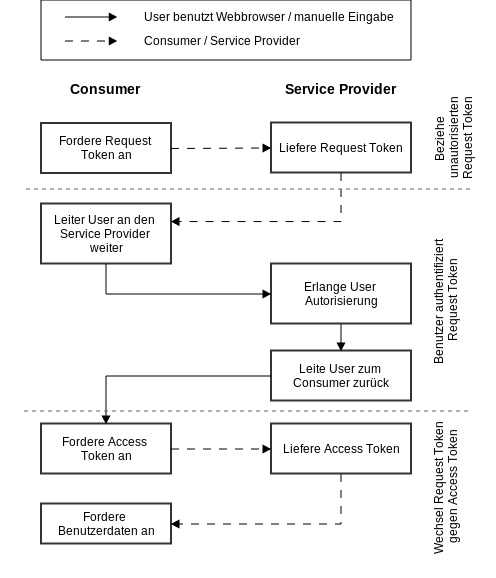
\includegraphics[scale=0.6]{resources/Bilder_Kapitel_2/oauth_workflow.png}
  \caption[Workflow des OAuth 1.0 Authentifizierungsprozesses]{Workflow des OAuth 1.0 Authentifizierungsprozesses (In Anlehnung an \cite{oauthdiagramm07})}
  \label{fig-oauth-workflow}
\end{figure}

In der Praxis würde sich der User beispielsweise für ein Textverarbeitungsprogramm von Google, welcher in diesem Fall der Consumer ist, interessieren.
Die Dateien, die er bearbeiten möchte, liegen jedoch bei Dropbox, dem Service Provider.
Der User möchte nun Google für den Zugriff auf seine Daten bei Dropbox berechtigen.
Dropbox verwendet eine offene \ac{API}, welche OAuth unterstützt und Google hat bereits bei dieser eine Entwickleranwendung angelegt.
Nach dem Anlegen hat Google die \frqq client credentials\flqq\ für seine Anwendung erhalten.

Wenn der User nun Google dazu berechtigen möchte, auf seine Benutzerdaten zugreifen zu können, muss er dazu einen Button auf der Webseite von Google betätigen.
Daraufhin werden zwei Vorgänge durchgeführt.
Zuerst schickt Google seine \frqq client credentials\flqq\ an Dropbox und erhält, insofern diese Gültig sind, die \frqq temporary credentials\flqq\ zurück.
Sobald Google diese erhalten hat, wird der User auf die Loginseite von Dropbox weitergeleitet.
Dort gibt er seine Zugangsdaten ein, um seine Authentizität zu beweisen.
Nachdem er eingeloggt ist, bekommt er eine Bestätigungsseite angezeigt, auf der er Google Zugriff auf seine Daten gewähren kann.
Hat er dem zugestimmt, wird er zu Google zurückgeleitet.
Google erhält daraufhin den \frqq request token\flqq\ zurück, welcher ihm aufzeigt, dass ihm der User den Zugriff gewährt hat.
Abschließend schickt Google seinen \frqq consumer key\flqq\ und den \frqq request token\flqq\ an Dropbox und erhält die \frqq token credentials\flqq .
Mit diesen kann Google fortan die Benutzerdaten von Dropbox abrufen, verändern und die gewünschten Textdateien des Users in seinem Service einbinden.
Im OAuth 1.0 Standard ist jedoch kein Parameter angegeben, welcher den Gültigkeitszeitraum der \frqq token credentials\flqq\ festlegt.
Somit sind diese für immer gültig oder entsprechend der Implementierung des Service Providers werden diese nach einem gewissen Zeitraum verworfen.
Jedoch gibt es keine Vereinheitlichung in diesem Punkt.

\subsection{OAuth 1.0A}
Nachdem im Jahr 2009 eine Sicherheitslücke in der OAuth 1.0 Methode entdeckt wurde, haben Google und Yahoo! eine weitere Revision von OAuth 1.0, welche später als OAuth 1.0A veröffentlicht wurde, entwickelt\cite[vgl.][]{oauth10a}.
Der Angriff auf das Authentifizierungsverfahren, welcher als \frqq session fixation attack\flqq\ bezeichnet wird, hat folgenden Ablauf.

Der Angreifer Mallory möchte ein Textdokument aus seiner Dropbox mit dem Google Textbearbeitungsprogramm bearbeiten.
Er initiiert dazu den OAuth Autorisierungsprozess bei Google, unterbindet jedoch die Weiterleitung zu Dropbox und speichert sich den Link dahin ab.
Dieser enthält die \frqq client credentials\flqq\ und die URL zur Authentifizierungsseite.
Nachfolgend bringt er einen Benutzer Alice dazu, diesen Link anzuklicken.

Alice führt den von Mallory gestarteten Autorisierungsprozess fort und wird zu Dropbox geleitet.
Dort gibt sie ihre Benutzerdaten ein und akzeptiert die Berechtigung der Google \ac{App} Zugriff auf ihre Daten zu haben.
Sie bekommt jedoch nicht mit, dass ein Angriff durchgeführt wird, da sie sich beim gültigen Serviceprovider befindet und auch die korrekte \ac{App} angezeigt bekommt.
Nachdem Alice zurück zur Applikation geleitet wurde, führt Mallory seinen Autorisierungsprozess fort, indem er die Weiterleitung von Dropbox zurück zu Google nachbaut oder diese bei Alice manipuliert.
Von diesem Zeitpunkt an ist der Dropbox-Account von Alice mit der Google \ac{App} von Mallory verbunden.

Das ganze Verfahren ähnelt einem Pishingverfahren und setzt auf Social Engineering, was bedeutet, dass das Vertrauen und die Gewohnheit eines unachtsamen Benutzers ausgenutzt wird und dieser einem Link aus einer nicht vertrauenswürdigen Quelle folgt.

Um diese Sicherheitslücke zu schließen, wurde als vorzeitige Lösung ein Warnhinweis vom Serviceprovider, also im Beispiel Dropbox, angezeigt, wenn der Benutzer von einer \ac{URL} weitergeleitet wurde, die nicht mit der \ac{URL} des \ac{App} Betreibers übereinstimmt, im Beispiel Google\cite[vgl.][]{session-fixation-attack}.
Diese Variante hat sich jedoch als unzureichend herausgestellt, sodass das OAuth 1.0A Protokoll entwickelt wurde.

In OAuth 1.0A wurden drei wesentliche Änderungen durchgeführt.
Wenn der Consumer die \frqq temporary credentials\flqq\ beim Service Provider anfordert, muss er eine Callback URL angeben\cite[vgl.][]{oauth10a}.
Dieser Parameter existierte bereits in der OAuth 1.0 Spezifikation, war dort aber optional und wurde erst beim Weiterleiten zum Service Provider mitgesendet, wenn die \frqq session fixation attack\flqq\ bereits gestartet ist.
Nach Abschluss der Autorisierung beim Service Provider wird der User an diese URL weitergeleitet.

Weiterhin wurde der Parameter \frqq oauth\_callback\_confirmed\flqq\ eingeführt, der den Wert true hat und bei der Anfrage des \frqq request token\flqq\ an den Consumer geschickt wird\cite[vgl.][]{oauth10a}.
Dieser dient lediglich zur Erkennung einer OAuth 1.0A Unterstützung Seitens des Service Providers.

Die letzte Änderung betrifft die Weiterleitung des Users vom Service Provider zum Consumer.
Hierbei wird der Parameter \frqq oauth\_verifier\flqq\ implementiert, der vom Consumer entgegengenommen und bei der Anfrage der \frqq token credentials\flqq\ mitgeschickt werden muss\cite[vgl.][]{oauth10a}.

Diese drei Änderungen haben die \frqq session fixation attack\flqq\ ungültig gemacht.
Das OAuth Komitee hat darüber hinaus jedem Anbieter dringendst geraten sein System auf OAuth 1.0A zu aktualisieren\cite[vgl.][]{session-fixation-attack}.

\subsection{OAuth 2.0}
\label{authentifizierung-oauth-2}
OAuth 2.0 wurde im Oktorber 2012 veröffentlicht und ist ein komplett neues Protokoll, welches nicht abwärtskompatibel zu OAuth 1.0 oder OAuth 1.0A ist\cite[vgl.][]{eran10}.
Es gibt wesentliche Veränderung im Workflow und in der Kommunikation mit dem Server.
Dabei sind drei Unterschiede als besonders prägnant zu erachten.
Jegliche Verbindungen erfolgen über \ac{SSL} und es muss keine eigene Signatur, wie bei den vorherigen OAuth Protokollen, erzeugt und geprüft werden\cite[vgl.][]{oauth12}.

Des Weiteren existiert nur noch ein Token in den \frqq token credentials\flqq .
Dieser wird \frqq access\_token\flqq\ genannt und dient fortan zur Authentifizierung des Users\cite[vgl.][]{oauth12}.
Ein optionaler \frqq refresh\_token\flqq\ kann vom Service Provider an den Consumer geschickt werden, welcher oftmals mit einem Parameter \frqq expires\_in\flqq\ übergeben wird\cite[vgl.][]{oauth12}.
Letzterer gibt in Millisekunden an, wie lange der \frqq access\_token\flqq\ gültig ist\cite[vgl.][]{oauth12}.
Sollte dieser abgelaufen sein, so kann ohne das Eingreifen des Users mithilfe des \frqq refresh\_token\flqq\ ein Neuer angefordert werden.
Ein weiterer Vorteil dieses Prinzips ist, dass die Laufzeit der \frqq token credentials\flqq\ explizit festgelegt wird und diese nicht wie bei OAuth 1.0 einen unbegrenzten Verwendungszeitraum ermöglichen.
Häufig wird dieser Zeitraum auf 3600 Millisekunden, also eine Stunde, festgesetzt.
Das OAuth Komitee empfiehlt dringend die Implementierung des \frqq refresh\_token\flqq\ und des \frqq expires\_in\flqq\ Parameters, jedoch sind beide optional, womit die Entscheidung beim Service Provider liegt, diese zu verwenden oder nicht\cite[vgl.][]{oauth12}.

Weiterhin gibt es vier Rollen im OAuth 2.0 Standard.
Es gibt den \frqq resource owner\flqq , welcher dem User entspricht, also einem Benutzer einer Anwendung\cite[vgl.][]{oauth12}.
Ebenfalls gleich geblieben ist der Client, welcher auch als Consumer bezeichnet wird\cite[vgl.][]{oauth12}.
Neu ist die Unterteilung in einem \frqq resource server\flqq\ und einem \frqq authorization server\flqq\cite[vgl.][]{oauth12}.
Der \frqq resource server\flqq\ hält die Benutzerdaten vor, während der \frqq authorization server\flqq\ die \frqq credentials\flqq , also jegliche Token speichert\cite[vgl.][]{oauth12}.
Diese Unterteilung erleichtert die Implementierung des Protokolls auf Seiten des Server Providers, der meist beide Rollen zugleich einnimmt.
Lediglich die Domain kann voneinander abweichen.

Der Workflow von OAuth 2.0 hat sich in der Praxis wie folgt verändert.
Wie bereits in den vorherigen Spezifikationen muss der Consumer eine Entwicklerapp beim Service Provider anlegen.
Dabei muss er bereits eine Callback \ac{URL} definieren, an die der User nach dem Autorisierungsprozess weitergeleitet wird.
Der Consumer erhält nach Abschluss der Erstellung die \frqq client credentials\flqq , also eine \frqq client\_id\flqq\ , sowie ein \frqq client\_secret\flqq .
Sobald ein User einen Consumer Autorisieren möchte, Zugriff auf seine Daten zu erhalten, wird er wie gewohnt zum Service Provider weitergeleitet.
Jedoch entfällt der bisherige Prozess zum Erzeugen der \frqq temporary credentials\flqq .
Der Consumer schickt lediglich seine \frqq client\_id\flqq\ bei Weiterleiten an den Service Provider, wodurch dieser die entsprechende Entwicklerapp eruieren kann.

Beim Service Provider bekommt der Benutzer, wie zuvor, die Loginseite angezeigt und muss nach erfolgreichem Login der Entwicklerapp den Zugriff gewähren oder diesen ablehnen.
Sobald er zugestimmt hat, wird er an die Callback \ac{URL} des Consumers geleitet, welche bei der Erstellung der Entwicklerapp definiert wurde.
Dabei wird ein Parameter mit der Bezeichnung \frqq code\flqq\ mitgeschickt.
Zum Erzeugen eines \frqq access\_tokens\flqq\ muss dieser, samt der \frqq client\_id\flqq\ an den Service Provider geschickt werden.
Dieser überprüft den \frqq code\flqq\ und schickt den \frqq access\_token\flqq , sowie optional den \frqq refresh\_token\flqq\ und die Lebenszeit des \frqq access\_tokens\flqq\ an den Consumer zurück.
Ein Beispiel für solch eine Antwort ist in Quellcode \ref{fig-oauth-response} zu sehen.

\begin{lstlisting}[label=fig-oauth-response,caption={[Aufbau eines Response vom Service Provider an den Consumer]Aufbau eines Response vom Service Provider an den Consumer\cite{oauth12}}]
HTTP/1.1 200 OK
Content-Type: application/json;charset=UTF-8
Cache-Control: no-store
Pragma: no-cache

{
    "access_token":"2YotnFZFEjr1zCsicMWpAA",
    "token_type":"example",
    "expires_in":3600,
    "refresh_token":"tGzv3JOkF0XG5Qx2TlKWIA",
    "example_parameter":"example_value"
}
\end{lstlisting}

Der Consumer kann nun mit den erhaltenden \frqq access\_token\flqq\ auf die Benutzerdaten zugreifen.
Sollte die Lebenszeit des Tokens abgelaufen sein, muss dieser unter Zuhilfenahme des \frqq refresh\_tokens\flqq\ neu angefordert werden.
Das bedeutet, der Consumer macht einen Request mit dem \frqq refresh\_token\flqq\ und der \frqq client\_id\flqq\ an den Service Provider und dieser schickt, sowohl einen neuen \frqq access\_token\flqq , als auch einen neuen \frqq refesh\_token\flqq\ und ein \frqq expires\_in\flqq\ an die Anwendung zurück.
Dieses Verfahren kann beliebig oft wiederholt werden.

%\section{Programmierumgebung}
\subsection{node.js}
\subsection{Zusammenfassung}

% module
    % Lizenzen der module -> Problem, weil einfach nachgealden
% package.json
% 

% Chapter 2
\chapter{Anforderungsanalyse}
\label{anforderungsanalyse}

Die bisher erarbeiteten Grundlagen sollen in diesem Kapitel dazu dienen, die Anforderungen für die zu entwickelnde Anwendung zu formulieren.
Dabei werden Aspekte betrachtet, die bei der konkreten Umsetzung relevant sein werden.

\section{Systemanforderung}
\label{anforderungcloudgrid}
Mit CloudGrid soll ein Prototyp für eine Desktopapplikation erstellt werden, der es dem Benutzer ermöglicht, verschiedene Cloudservices zu einem einzigen System zusammenzufassen.
Dieses soll auf einem \ac{RAID} ähnlichen Prinzip basieren, dass bedeutet, dass Dateien redundant auf mehreren Services gespeichert werden sollen.
Der Vorteil für den Benutzer liegt darin, dass ihm durch diese Vereinigung einerseits mehr Speicherplatz zur Verfügung steht, andererseits eine größere Ausfallsicherheit gewährleistet werden kann.
Selbst wenn ein Anbieter seinen Dienst einstellt oder temporär nicht verfügbar ist, so ist es dem Nutzer somit noch möglich, weiterhin Zugriff auf seine Daten zu erhalten.
Die gesamte Dateiverwaltung soll auf dem Client durchgeführt werden.
Es wird bewusst auf einen Serverdienst verzichtet, welcher die Verwaltungslogik der verschiedenen Services übernimmt.
Dadurch soll das System für den Benutzer nachvollziehbarer sein, da er sich nicht bei einem weiteren Dienst anmelden muss und ihm mehr Kontrolle über den Verbleib seiner Daten geben.

Neben dem Zusammenschluss mehrerer Cloudservices, ist das Dateihandling eine weitere zentrale Aufgabe von CloudGrid.
Hierbei soll ein, vom Benutzer festgelegter Ordner auf Veränderungen überprüft werden.
Dazu zählen auch Unterordner mit beliebiger hierarchischer Tiefe.
Wenn eine Veränderung festgestellt wird, sollen mehrere Dateioperationen durchgeführt werden.
Das bedeutet konkret, dass vor dem Upload einer Dateien, diese clientseitig komprimiert und somit der Upload beschleunigt werden soll.
Um die Datensicherheit zu erhöhen, wird die Datei darüber hinaus beim Client verschlüsselt.
Der Benutzer verschickt dadurch keine unverschlüsselten Dateien, welche beispielsweise durch Angriffe von einem Hacker abgefangen und ausgelesen werden könnten.
Weiterhin liegt die Datei verschlüsselt beim dem Cloudanbieter, wodurch dieser keine Möglichkeit hat, den Inhalt der Datei einzusehen.
Um diesen Aspekt noch zu verstärken, wird die Datei in mehrere Teilstücke fragmentiert, um diese daraufhin, wie bereits erwähnt, redundant auf verschiedenen Anbietern zu speichern.
Bei sensiblen Daten, wie beispielsweise Dokumenten mit Passwörtern, trägt dieses Verfahren nur bedingt zur Dateisicherheit bei, da weiterhin Informationen über den Inhalt gewonnen werden können.
Jedoch erschwert es einem potentiellen Angreifer Einsicht in die komplette Datei zu erhalten.
Wird hingegen eine Datei gelöscht, muss das ebenfalls von CloudGrid erkannt werden und entsprechend alle Dateien auf den Cloudservices gelöscht werden.

Der zu erstellende Prototyp wird darüber hinaus nur eine Synchronisierung mit einem Client unterstützen.
Die Synchronisierung mit mehr als einem Client setzt ein komplexes Dateimanagement voraus, welches den Rahmen dieser Arbeit überschreiten würde.

\section{Cloudanservices}
\label{anfoderungcloudanbieter}
Das Programm CloudGrid soll, wie bereits beschrieben, eine Verbindung mit mehreren Cloudanservices aufnehmen können.
Dazu müssen zuvor relevante Dienste evaluiert werden.
Dabei wurden folgende Kriterien als ausschlaggebend erachtet:
\paragraph{Serviceart:} CloudGrid unterstützt ausschließlich Services, welche sich als Online-Speicher verstehen.
Services wie beispielsweise Evernote oder Spotify, welche ebenfalls als Cloudservices angesehen werden, werden nicht unterstützt.
\paragraph{Lizenzmodell:} Ein potenzieller Clouddienst muss über einen kostenlosen Service verfügen.
Dennoch soll CloudGrid darauf ausgelegt sein, kostenpflichtige Services einbinden zu können.
Auf eine ausführliche Analyse kann in dieser Arbeit aus finanzieller Sicht nicht eingegangen werden.
\paragraph{Programmierschnittstelle:} Die Programmierschnittstelle, auch \ac{API} genannt, des Anbieters muss für Nutzer des kostenfreien Services verfügbar sein.
Einige Anbieter bieten ihre Schnittstelle nur an, wenn der Benutzer einen kostenpflichtigen Service in Anspruch nimmt.
Das ist sowohl für den Nutzer nachteilig, da er, falls er den Dienst zuvor testen möchte, diesen nicht in CloudGrid einbinden kann, als auch im Rahmen dieser Arbeit finanziell nicht realisierbar.
Anbieter die über keine \ac{API} verfügen, werden darüber hinaus nicht vom Programm unterstützt.
Bei der Umsetzung des Prototypen wird lediglich \ac{JSON} als Datenformat zugelassen, da dieses von vielen Anbietern verwendet wird.
\paragraph{Authentifizierungmethoden:} Der Service muss über eine OAuth Authentifizierung verfügen.
Diese kann sowohl in Version 1.0, 1.0A, als auch 2.0 vorliegen.
Alle drei Versionen sollen in CloudGrid vollständig implementiert werden.
Eigene Authentifizierungsverfahren sind aufwändiger zu integrieren und für den Prototypen nicht vorgesehen.
\paragraph{Rechtliche Anforderungen:} Die rechtlichen Aspekte bei der Entwicklung von CloudGrid spielen eine elementare Rolle.
Hierbei muss betrachtet werden, ob die AGB's der Anbieter, Programme, wie das zu entwickelnde System, einschränken oder sogar verbieten.
Weiterhin muss geprüft werden, ob und inwiefern der Anbieter Rechte an den Daten erhält.
Zudem wird geprüft, ob etwaige Limitierungen, wie eine bestimmte Anzahl von maximalen Requests, bei der Nutzung der \ac{API} existieren.

\section{Technologien}
\label{anforderungtech}
Nachdem die Rahmenbedingungen für die Cloudservices definiert wurden, soll auch auf die technologischen Anforderungen von CloudGrid eingegangen werden.

Bei der Wahl der Programmierumgebung wird besonderer Wert auf eine schnelle Bearbeitung des Filesystems gelegt.
Dies ist besonders wichtig, da CloudGrid viele Dateioperationen durchführen muss und der Nutzer nicht unnötig lange auf diese warten soll.
Da das Programm als Dienst im Hintergrund permanent ausgeführt wird, ist es darüber hinaus wichtig, dass zur Laufzeit nicht unnötig viele Ressourcen verbraucht werden.
Nicht zuletzt soll eine plattformunabhängige Entwicklung möglich sein.

Das \ac{GUI} soll dem Benutzer zur Verwaltung von CloudGrid dienen.
Als wichtig bei der Wahl der Umgebung wird eine für den Benutzer gewohnte Umgebung erachtet.
Er soll sich schnell in diese einfinden und alle relevanten Informationen erhalten.
Beim ersten Start von CloudGrid erhält der Benutzer die Möglichkeit persönliche Einstellungen zu tätigen.
Dazu zählt das Festlegen des zu überwachenden Ordners, Einbinden der Cloudservices und eine kurze Einführung in die Funktionalität von CloudGrid.
All diese Einstellungen können später noch bearbeitet werden.
Nachdem die grundlegende Initialisierung abgeschlossen ist, erhält der Benutzer die Möglichkeit Auskunft über durchgeführte Dateioperationen und dem Fortschritt des Dateiuploads zu bekommen.
Darüber hinaus kann er sich Informationen zu den eingebundenen Cloudservices anzeigen lassen, wie beispielsweise die Auslastung des Speicherplatzes bei diesem Anbieter oder eine Liste der hochgeladenen Dateien.

Zusätzlich soll es Entwicklern möglich sein, die \ac{GUI} anzupassen und um eigene Funktionalitäten zu erweitern.

Auch bei der Wahl der \ac{GUI} ist die Plattformunabhängigkeit ein wichtiger Aspekt.
Die \ac{GUI} soll sich auf allen Systemen gleich verhalten und sich optisch nicht oder nur gering unterscheiden.

Alle Einstellungen von CloudGrid und Einstellungen, die vom Benutzer getätigt wurden, sollen lokal beim Client vorgehalten und nicht mit einem weiteren Dienst synchronisiert werden.
Das hat den Vorteil, dass der Benutzer seine Informationen nicht an einen Drittanbieter weitergeben muss und somit eine größere Dateiintegrität gewährleistet wird.
Neben den allgemeinen Einstellungen sollen auch die Dateiinformationen, wie beispielsweise die Verteilung der Teilstücke einer Datei auf den verschiedenen Cloudservices, deren Passphrase zum Entschlüsseln der Datei und die Hashwerte der originalen Datei gespeichert werden.
%Zusätzlich wird die Ordnerstuktur des zu überwachenden Ordners in der Datenbank gespeichert.
Außerdem sollen Informationen über die einzelnen Provider gespeichert werden, wie beispielsweise die App-Token zum Authentifizieren.
Zur Speicherung der Daten muss daher ein geeignetes Datenbanksystem evaluiert werden.
Dieses soll sich vom Programmierer leicht in die Anwendung integrieren lassen und ohne großen initialen Aufwand eingerichtet werden können.
\newpage
\section{Use-Case-Analyse}
\label{anforderungusecase}
In der Use-Case-Analyse sollen beispielhaft vier Fälle aufgezeigt werden, welche bei der Benutzung von CloudGrid auftreten können.

\paragraph{Standardverhalten:}
Der Benutzer startet CloudGrid.
Daraufhin überwacht die Anwendung den zuvor ausgewählten Ordner auf Veränderungen.
Nun bearbeitet der Benutzer eine Datei.
CloudGrid erkennt eine Veränderung am Filesystem und zusätzlich, dass es sich dabei um eine Bearbeitung einer Datei handelt.
Die Datei wird daraufhin komprimiert, gesplittet und die Teilstücke verschlüsselt.
Dateiinformationen über die Teilstücke werden daraufhin in die lokale Datenbank gespeichert und die Teilstücke anschließend zu den jeweiligen Anbietern geuploaded.

\paragraph{Dateiänderung vor Programmstart:}
Der Benutzer bearbeitet eine Datei, bevor CloudGrid gestartet wurde.
Beim Start der Anwendung wird die Ordnerüberwachung gestartet.
Daraufhin werden die bestehenden Dateien auf Veränderung überprüft.
%Dazu werden die Hashwerte aus der Datenbank mit den Hashwerten der Dateien, welche zur Laufzeit berechnet werden, verglichen.
Zudem wird geprüft, ob neue Dateien hinzu gekommen sind oder bestehende gelöscht wurden.
Sollte eine Dateiänderung erkannt werden, werden die zuvor genannten Dateioperationen durchgeführt und die Teilstücke geuploaded.

\paragraph{Dateiänderung ohne Internetverbindung:}
Der Benutzer startet CloudGrid und zu diesem Zeitpunkt besteht eine Internetverbindung.
Die Ordnerüberwachung wird gestartet.
Daraufhin wird die Verbindung mit dem Internet getrennt.
CloudGrid wird in den Offline Modus geschaltet.
Das bedeutet, dass alle aktiv laufenden Dateioperationen abgebrochen werden und die Ordnerüberwachung gestoppt wird.
Sobald die Internetverbindung wiederhergestellt ist, ermittelt die Anwendung alle durchgeführten Veränderungen und führt entsprechend die Dateioperationen durch.

\paragraph{Teilstück wird auf Server gelöscht:}
Der Benutzer löscht ein Teilstück einer Datei direkt beim Cloudservice A.
CloudGrid wird vom Benutzer gestartet.
Die Anwendung prüft anhand der lokalen Datenbank, ob es Veränderungen bei den Cloudservices gibt.
Die Löschung des Teilstücks bei Cloudservice A wird erkannt und geprüft, bei welchem Anbieter die Datei redundant gespeichert wurde.
Daraufhin wird diese von Cloudservice B heruntergeladen, beim Benutzer zwischengespeichert und zum Cloudservice A erneut hochgeladen.
Sollte das Teilstück auf beiden Services nicht mehr existieren, so werden alle Teilstücke der Datei auf allen Services gelöscht.
Daraufhin werden die Dateioperationen auf der lokalen Datei beim Client durchgeführt und die Teilstücke erneut geuploaded.

\section{Abgrenzung zu bestehenden Systemen}
\label{anforderungabgrenzung}
Im folgenden Abschnitt sollen Abgrenzungen zu verschiedenen bestehenden System aufgezeigt werden.
Es werden nur Dienste betrachtet, die auf bestehende Cloudservices aufsetzen und diese um Funktionen, wie das Verschlüsseln von Dateien oder den Zusammenschluss mehrerer Dienste, erweitern.

\paragraph{Boxcryptor:}
Boxcryptor ist ein Programm, um Daten bei verschiedenen Cloudanbietern zu verschlüsseln.
Dabei beschränkt sich dieser Dienst auf einen Anbieter.
Eine Vereinigung mehrerer Dienste, wie bei CloudGrid, ist nicht gegeben.
Darüber hinaus wird ein Benutzerkonto beim Anbieter benötigt.
Die Dateien werden auf Benutzerseite verschlüsselt.
Da jedoch der Anbieter potentiell die Möglichkeit hat, die Dateien durch seinen Dienst zu entschlüsseln, ist die Dateisicherheit nur bedingt gegeben.
Der Vorteil liegt jedoch darin, dass sowohl ein Programm für die Nutzung auf Desktoptrechnern verfügbar ist, als auch \acp{App} für mobile Endgeräte wie Android und iOS.
Um eine erweiterte Version von Boxcryptor verwenden zu können, muss ein kostenpflichtiger Premium Account gekauft werden.
Dieser beinhaltet Funktionen wie die Nutzung von mehr als zwei Geräten oder die Verschlüsselung von Dateien auf mehr als einem Cloudservices.

\paragraph{Cloudii:}
Cloudii ist eine Android \ac{App}, die es dem Benutzer ermöglicht, mehrere Clouddienste zu verwalten.
Dabei ist es möglich, Daten redundant zu speichern, jedoch nicht diese zu verschlüsseln.
Weiterhin ist die Anwendung ausschließlich für Android verfügbar, was Benutzer mit anderen Systemen ausschließt.

\paragraph{Otixo:}
Das ist eine kostenpflichtige Webapplikation, welche die Verwaltung von Dateien über mehrere Cloudanbieter ermöglicht.
Dabei ist eine redundante Speicherung der Daten ebenso wenig möglich, wie die Verschlüsselung selbiger.

\paragraph{Primadesk:}
Auch Primadesk ist eine kostenpflichtige Webapplikation, bei der es ebenso wie bei Otixo, nicht möglich ist, Dateien zu verschlüsseln oder redundant zu speichern.
Jedoch werden mobile \acp{App} sowohl für Android als auch für iOS angeboten.

\paragraph{Cloudfuze:}
Cloudfuze ist eine reine Desktopapplikation, die ebenfalls kostenpflichtig ist.
Auch diese Anwendung dient nur der Verwaltung mehrerer Clouddienste.
Daher bietet sie einen ähnlichen Funktionsumfang wie Otixo oder auch Primadesk.

\paragraph{TrueCrypt:}
Neben den bisher vorgestellten Anwendungen gibt es auch lokale Lösungen zum Verschlüsseln der Daten.
Eine Möglichkeit besteht darin Ordner mittels TrueCrypt zu verschlüsseln.
Die Anwendung erzeugt aus den verschlüsselten Daten einen Container, welcher als virtuelle Festplatte von dem Programm selbst gemountet werden kann.
Sowohl zum Verschlüsseln, als auch zum mounten, muss der Benutzer ein festgelegtes Passwort eingeben.
Mit der Methode kann der Benutzer den Ordner, welcher von dem Cloudservices synchronisiert wird, Verschlüsseln und nur den Container zum Anbieter hochladen.
Dadurch sind die Daten geschützt, jedoch lassen sich somit nicht mehrere Cloudanbieter zusammenfassen.
Auch die Ausfallsicherheit ist bei dieser Methode nicht gewährleistet.

Darüber hinaus muss der Benutzer bei TrueCrypt zuvor die Größe des Containers bestimmen.
Das bedeutet, dass selbst wenn nur eine Textdatei in einem Container liegt, die Gesamtgröße der Datei festgelegt ist.
Somit ergibt sich ein Overhead und die Uploadzeit steigt, je nach gewählter Dateigröße, stark an.
Ein weiterer Nachteil ist, dass auf jedem Gerät, welches dieses Verfahren verwendet, TrueCrypt installiert sein muss, um den Inhalt der Dateien betrachten zu können.
Es gibt mittlerweile auch mobile \acp{App}, die TrueCrypt-Container entschlüsseln, jedoch ist eine Verwaltung im Web derzeit nicht möglich.

Es lässt sich festhalten, dass die vorgestellten Dienste Cloudservices um sinnvolle Funktionalitäten erweitern.
Jedoch bietet keiner dieser Dienste die Funktionsvielfalt von CloudGrid.
Die meisten der hier vorgestellten Dienste verbinden mehrere Services zu einem gemeinsamen, beziehungsweise ermöglichen die gleichzeitige Verwaltung mehrerer Services.
Dabei wird wenig Wert auf die Dateisicherheit gelegt.
Darüber hinaus sind viele Dienste nur mit einem kostenpflichtigen Abonnement im vollen Umfang nutzbar.
Auch das Verfahren von TrueCrypt löst lediglich die Problematik der Dateisicherheit auf einem Service, jedoch nicht die Verknüpfung und redundante Speicherung über mehrere Anbieter.
Weiterhin setzen alle Dienste, bis auf die TrueCrypt Methode, eine Registrierung bei dem entsprechenden Anbieter voraus.
Eine rein clientseitige Verwaltung der Daten, wie es bei CloudGrid der Fall sein wird, liegt damit also nicht vor.

% Chapter 3
\chapter{Systementwurf}
\label{systementwurf}
Im folgenden Kapitel werden die von CloudGrid verwendeten Komponenten, unter Beachtung der zuvor definierten Anforderungen, beschrieben.
Dazu wird zuerst die verwendete Programmierumgebung analysiert, da diese für die weiteren Abschnitte relevant sein wird.
Danach werden mögliche Cloudservices evaluiert und auf deren rechtliche Bedingungen eingegangen.
Darauf aufbauend wird die Architektur des Systems aufgezeigt und die einzelnen Schichten der Architektur des Systems beschrieben.

% #########################################################
% ################## Programmierumgebung ##################
\section{Programmierumgebung}
\label{systementwurf-programmierumgebung}
Die Wahl der Programmierumgebung ist maßgeblich für die Anwendung.
Dabei richtet sich sowohl die Umsetzung der Benutzeroberfläche, als auch die Wahl möglicher Plugins und Bibliotheken, nach selbiger.
Unter Berücksichtigung der Kriterien aus Abschnitt \ref{anforderungtech} wurden die folgenden Programmierumgebungen analysiert.

\paragraph{C:}
Die Vorteile von C liegen bei der Effizienz im Umgang mit dem Filesystem und der direkten Manipulation des Arbeitsspeichers.
Als Nachteil hingegen ist das Fehlen der objektorientierten Programmierung zu nennen.
Dadurch ist es schwieriger, sowohl den Quellcode modular aufzubauen, als auch für andere Entwickler eigene Module in die Anwendung zu integrieren.
Darüber hinaus gibt es nur wenige Bibliotheken zum Verarbeiten von \ac{HTTP} Requests.
Zudem ist die Lernkurve für die \ac{GUI} Entwicklung steil und erfordert fundiertes Vorwissen in der jeweiligen Bibliothek.
Ein weiterer Nachteil ist es, dass mit C keine plattformunabhängige Programmierung möglich ist.
Der Programmierer muss viele Sonderfälle berücksichtigen und somit Anpassungen für das jeweilige Zielsystem einbauen.

\paragraph{\cpp :}
Diese ist der Funktionsweise von C sehr ähnlich.
Dadurch entstehen ähnliche Vor- und Nachteile.
Beispielsweise arbeitet diese ähnlich effizient mit dem Filesystem, hat aber auch dieselben Nachteile was die plattformunabhängige Programmierung betrifft und eine ähnlich steile Lernkurve wie bei C.
Lediglich die Unterstützung von Objektorientierung ist als großer Vorteil zu vermerken.

\paragraph{Java:}
Anders als die beiden bisher vorgestellten Programmiersprachen, wird Java nicht direkt vom Betriebssystem ausgeführt, sondern in der Java Virtual Machine.
Der Vorteil dabei ist, dass die Sprache dadurch plattformunabhängig ist.
Jedoch gestaltet sich dadurch die Arbeit auf dem Filesystem als weniger effizient.
Zudem belegt die Java Virtual Machine sowohl erheblich viel Arbeitsspeicher, als auch Prozessorleistung, da sie zum Ausführen von Javaprogrammen mit gestartet und im Hintergrund ausgeführt wird.
Ähnlich wie \cpp\ ist Java objektorientiert, was die Erweiterung des Systems für Entwickler leichter macht.
Dank der Apache Commons\footnote{\url{http://commons.apache.org}}, einer Klassenbibliothek der Apache Inc., werden viele Standardfunktionen nachgeliefert.
Somit wird ein gutes \ac{HTTP} Handling und auch das Handling von OAuth Request ermöglicht.
Auf Seiten der \ac{GUI} gibt es die selben Probleme wie bei C und \cpp .

\paragraph{Node.js:}
Diese recht junge Entwicklungsumgebung, welche auf der Google JavaScript Engine V8\footnote{\url{https://code.google.com/p/v8}} basiert.
Diese ist in \cpp\ geschrieben, sodass Node.js damit letztendlich auf \cpp\ aufsetzt.
Das ermöglicht eine effiziente Bearbeitung des Filesystems und des Speicherzugriffs.
Ein Programm wird in JavaScript geschrieben, kann aber darüber hinaus über \cpp\ Module verfügen.
Node.js ist für alle gängigen Betriebssysteme, Windows, Mac OS X und Linux, verfügbar.
Der primäre Anwendungsbereich ist die Funktion als Webserver.
Jedoch lassen sich auch Desktopanwendungen damit umsetzen.
Durch die Webserverfunktionalität kann die \ac{GUI} der Anwendung komplett mit \ac{HTML} und \ac{CSS} im Browser umgesetzt werden.
Das gibt dem User eine gewohnte Arbeitsumgebung.
Node.js ist modular aufgebaut, sodass einzelne Plugins nachgeladen werden können.
Darüber hinaus können diese Plugins, sowie Node.js selbst, über ein einfaches Installationsskript bei dem Benutzer installiert werden.

\paragraph{Fazit:}
Unter Berücksichtigung der in Abschnitt \ref{anforderungtech} definierten Anforderungen und der in diesem Abschnitt evaluierten Programmierumgebungen, wird bei der Umsetzung von CloudGrid auf Node.js gesetzt.
Diese bietet die Vorteile einer effizienten Ausführung, wie beispielsweise \cpp\ und ermöglicht darüber hinaus eine plattformunabhängige Programmierung.
Durch die Darstellung im Browser wird dem Benutzer eine gewohnte Arbeitsumgebung ermöglicht, die ihm eine Einarbeitung in das System erleichtern soll.
Durch ein großes Angebot an Bibliotheken können darüber hinaus viele Funktionalitäten nachgeliefert werden, was den Programmieraufwand minimieren wird.

\section{Evaluation der Cloudservices}
\label{systementwurf-cloudanbieter}
Anhand der in Abschnitt \ref{anfoderungcloudanbieter} aufgeführten Kriterien sollen nun die Cloudservices evaluiert werden.
In Tabelle \ref{tabellecloudanbieter} werden mehrere Anbieter aufgelistet.
Zeilen, die grün hervorgehoben sind, erfüllen die Anforderungen und können potentiell in CloudGrid integriert werden.
Wohingegen rot hervorgehobene Zeilen, mindestens ein Kriterium nicht erfüllen und somit den Anforderungen nicht gerecht werden.

\begin{table}[htpb]
\centering
\begin{tabular}{| r | c c c c c |}
	\rowcolor{dunkelgrau}
	\hline
	Name               & kostenlos & Speicherplatz & offene API & API Format & OAuth    \\
	\hline
	\rowcolor{lightgreen}
	Dropbox            & ja        & 2 GB         & ja          & json        & 1.0/2.0 \\
	\rowcolor{lightgreen}
	Skydrive           & ja        & 25 GB        & ja          & json        & 2.0     \\
	\rowcolor{lightgreen}
	Google Drive       & ja        & 5 GB         & ja          & json        & 2.0     \\
	\rowcolor{lightgreen}
	Box                & ja        & 5 GB         & ja          & json        & 2.0     \\
	\rowcolor{lightgreen}
	Ubuntu One         & ja        & 5 GB         & ja          & json        & 1.0     \\
	\rowcolor{lightgreen}
	Computerbild-Cloud & ja        & 2 GB         & ja          & json        & 1.0A    \\
%	\rowcolor{lightgreen}
%	Wuala              & ja        & 5 GB         & ja          & ?           & nein    \\
    \rowcolor{lightred}
    MediaFire          & ja        & 10 GB        & ja          & json/xml    & nein    \\
	\rowcolor{lightred}
	Amazon S3          & ja        & 5 GB         & ja          & xml         & nein    \\
	\rowcolor{lightred}
	Amazon Cloud Drive & ja        & 5 GB         & nein        & -           & -       \\
	\rowcolor{lightred}
	Safesync           & nein      & -            & nein        & -           & -       \\
	\rowcolor{lightred}
	Teamdrive          & ja        & 2 GB         & nein        & -           & -       \\
	\rowcolor{lightred}
	iDrive             & ja        & 5 GB         & ja          & xml         & 1.0     \\
	\rowcolor{lightred}
	iCloud             & ja        & 5 GB         & nein        & -           & -       \\
%	\rowcolor{lightgreen}
%	mozy               & ja        & 2 GB         & ja          & ?           & ?       \\
	\rowcolor{lightred}
	liveDrive          & nein      & -            & ja          & xml         & nein    \\
	\rowcolor{lightred}
	ADrive             & ja        & 50 GB        & nein        & -           & -       \\
	\rowcolor{lightred}
	Telekom Cloud      & nein      & -            & ja          & xml         & 1.0     \\
	\rowcolor{lightred}
	CloudMe            & ja        & 3 GB         & ja          & xml         & nein    \\
	\rowcolor{lightred}
	CloudSigma         & nein      & -            & nein        & -           & -       \\
	\rowcolor{lightred}
	SugarSync          & nein      & -            & ja          & xml         & nein    \\
	\hline
\end{tabular}
\caption{Evaluierte Cloudservices}
\label{tabellecloudanbieter}
\end{table}
\newpage

Für den zu entwickelnden Prototypen werden daher die vier erstgenannten Services, Dropbox, Microsoft Skydrive, Google Drive, sowie Box, implementiert.
Diese erfüllen alle zuvor definierten Anforderungen, genau wie Ubuntu One und Computerbild-Cloud.
Jedoch sind die beiden letztgenannten, aus zeitlichen Gründen, nicht für die Umsetzung des Prototypen vorgesehen.
Die übrigen 13 Anbieter erfüllen nicht die Anforderungen an das System, weshalb auch diese nicht implementiert werden.
Um das Portfolio an Cloudservices für CloudGrid zu steigern, sollte jedoch in einer späteren Version die Unterstützung von \ac{XML} als \ac{API} Format in Betracht gezogen werden, sowie die Implementierung von Authentifizierungsverfahren abseits von OAuth.
Dadurch würden vier weitere Anbieter, Mediafire, Amazon S3, iDrive und CloudMe, aus der Tabelle \ref{tabellecloudanbieter} unterstützt werden.

\subsection{Authentifizierung}
\label{systementwurf-auth}
Die Authentifizierung mit den verschiedenen Cloudservices wird im Prototypen ausschließlich über OAuth 2.0 funktionieren.
Das Prinzip von OAuth wurde im Abschnitt \ref{oautheinleitung} beschrieben.
Bevor CloudGrid mit einem Service kommunizieren kann, muss eine Entwicklerapp bei dem Anbieter erstellt werden.
Diese verfügt über einen \frqq public\flqq\ und einen \frqq private Key\flqq , die zum Verbinden mit dem Service notwendig sind.

Das Problem bei diesem Konzept ist, dass vom Entwickler einer Anwendung keine vorgefertigten Entwicklerapps mitgeliefert werden können, da sowohl der public als auch der private Key im Klartext in der Anwendung gespeichert werden müssen und dann per \ac{HTTP} Request an den Server übertragen werden.
Dadurch wäre es möglich, diese auszulesen und die Entwicklerapp zu kompromittieren.
Einzige bisher bekannte Lösung ist der Einsatz eines Proxyservers, welcher zuvor den \ac{HTTP} Request entgegennimmt und um den private Key erweitert.
Dadurch wäre die Sicherheit des Keys gewährleistet, jedoch widerspricht das dem Konzept von CloudGrid, da es eine weitere Serverapplikation voraussetzt.
Zudem würde durch diesen Zwischenschritt die Ausführung der Anfrage verlangsamt werden.
Daher wird es in CloudGrid notwendig sein, dass der Benutzer selbständig eine Entwicklerapp anlegen muss und den public sowie den private Key in den Einstellungen von CloudGrid hinterlegt.
Das ist für die Bedienbarkeit ein großer Nachteil, jedoch schafft das Konzept von OAuth keine andere Möglichkeit.

Nachdem der User die Entwicklerapp erstellt hat und die Keys in den Einstellungen eingetragen hat, muss er lediglich einen Button in der \ac{GUI} anklicken, um die Authentifizierung durchzuführen.
Daraufhin öffnet sich ein Fenster, welches die Loginseite des jeweiligen Anbieters anzeigt.
Der User muss sich dort mit seinen Benutzerdaten anmelden und der Anwendung entsprechend den Zugriff gewähren.
Daraufhin ist CloudGrid berechtigt über die Anwendung mit dem Service zu kommunizieren.
In CloudGrid wird dazu ein Token gespeichert, der zur Identifizierung des Benutzers beim Service verwendet wird.
Der Token entspricht einer Session, sodass diese zeitlich begrenzt ist.
Das bedeutet, dass der Token in regelmäßigen Abständen neu angefordert werden muss.
Diese Aufgabe übernimmt CloudGrid eigenständig, sodass es keinen zusätzlichen Aufwand für den Nutzer erfordert.

\subsection{API}
\label{systementwurf-api}
Die Kommunikation über die \ac{REST} \ac{API} des Anbieters erfolgt mittels \ac{HTTP} Requests.
Insofern \ac{HTTPS} von den Anbietern unterstützt wird, kommunizieren auch CloudGrid über dieses Protokoll.
Als Rückgabewert einer Anfrage wird ein \ac{JSON} Response erwartet.
Dieser wird, von einer anbieterspezifischen Klasse in der Anwendung, entgegengenommen und ausgewertet.
Der Benutzer bekommt daraufhin beispielsweise Angaben zu seinem noch verfügbaren Speicherplatz, Informationen zu seinem Benutzerkonto oder auch eine Übersicht über die hochgeladenen Dateien, in der \ac{GUI} angezeigt.
Jegliche Dateioperationen, wie der Up- oder Download erfolgen ebenfalls über die \ac{API} und werden gleichermaßen durch die Klasse ausgeführt.

Der Upload einer Datei erfolgt bei den meisten Anbietern über einen \frqq multipart post\flqq\cite{multi95}.
Das bedeutet, dass sie als binär Daten und unter Verwendung eines speziellen \ac{HTTP} Headers zum Anbieter geschickt wird.
Als Resultat schickt der Anbieter einen JSON Response zurück, der Informationen über den Upload enthält.

\subsection{Rechtliche Aspekte}
\label{systementwurf-recht}
Bei der Betrachtung der rechtlichen Aspekte der vier ausgewählten Anbieter konnten ähnliche Sachverhalte identifiziert werden.

Jeder Anbieter behält sich das Recht vor Dateien des Benutzers zu deaktivieren oder zu löschen.
Dies kann entweder aufgrund einer Urheberrechtsverletzung oder durch den Verstoß gegen die \acp{AGB} oder die Datenschutzbestimmungen des Anbieters geschehen\cite[vgl.][]{box-terms, drop12, goog11, skyd12}.
Darüber hinaus Behalten sich alle Dienste das Recht vor, "`die Services jederzeit mit oder ohne Angabe von Gründen und mit oder ohne Benachrichtigung zeitweilig oder endgültig zu beenden"'\cite{drop12}.

Weiterhin sichert der Benutzer dem Anbieter zu, die Daten zur Wartung und zur Analyse der Dienste an Drittanbieter weiterzugeben\cite[vgl.][]{box-terms, drop13, goog11, skyd12}.
Das bedeutet konkreter, dass die Daten gescannt werden und sowohl der Anbieter selbst, als auch Drittanbieter, Zugriff zu den Inhalten der Dateien gewährt werden.
"`Bei der Bereitstellung, Analyse und Optimierung unseres Dienstes (z. B. Datenspeicherung, Wartungsdienste, Datenbankpflege, Webanalyse, Zahlungsabwicklung und Verbesserung der Funktionen des Dienstes) unterstützen uns gegebenenfalls vertrauenswürdige Drittunternehmen und Einzelpersonen. Diese Drittparteien haben möglicherweise Zugriff auf Ihre Informationen, allerdings nur sofern dies zur Durchführung der von uns beauftragten Tätigkeiten erforderlich ist und im Rahmen von Bedingungen, die den vorliegenden Datenschutzrichtlinien ähnlich sind"'\cite{drop12}.

Dabei geht aus den \acp{AGB} von Dropbox hervor, dass diese den Clouddienst Amazon S3 verwenden, sodass im Endeffekt die Daten des Nutzers bei der Amazon Web Services, Inc\footnote{\url{http://aws.amazon.com/de}} gelagert werden.
Microsoft Skydrive verwendet ebenfalls einen Drittanbieter, namens Wuala\footnote{\url{http://www.wuala.com}}, zum Speichern der Nutzerdaten.
Auch in diesem Fall speichert der Benutzer somit seine Daten nicht direkt beim eigentlichen Anbieter.
Lediglich box und Google Drive verwenden eigene Rechenzentren zum speichern der Daten\cite[vgl.][]{box-terms, goog11}.
Der Nachteil für den Benutzer bei Dropbox und Microsoft Skydrive ist die Abhängigkeit von einem weiteren Dienst.
Das bedeutet rechtlich, dass bei der Verwendung dieser zwei Dienste automatisch in die \acp{AGB} des Drittanbieters mit eingewilligt wird.
Letztendlich leidet die Nachvollziehbarkeit für den Benutzer darunter, da er weniger Kontrolle über den Verbleib seiner Daten hat und sich darüber hinaus in die \acp{AGB} mehrerer Anbieter einlesen muss.
Zudem geben alle Anbieter an, mit Strafverfolgungsbehörden zusammenzuarbeiten und im Falle eines gerichtlichen Beschlusses, die Daten des Nutzers offenzulegen\cite[vgl.][]{box-terms, drop12, goog11, skyd12}.

Als positiv ist jedoch zu verzeichnen, dass alle Anbieter angeben, dass sie keinen Anspruch auf das Urheberrecht der Dateien erheben\cite[vgl.][]{box-terms, drop12, goog11, skyd12}.
Microsoft hat folgenden Absatz in ihren Datenschutzbestimmungen: "`erheben wir keinen Anspruch auf das Eigentum an den Inhalten, die Sie über die Dienste bereitstellen. Ihre Inhalte bleiben Ihre Inhalte, und Sie sind für diese verantwortlich"'\cite{skyd12}.

Bei der Verwendung von Third-Party-\acp{App}, also Entwicklerapps, die von Drittanbietern angelegt werden und zur Kommunikation mit dem eigentlichen Cloudservice dienen, geben die Anbieter jegliche Verpflichtungen an den Drittanbieter ab.
Dropbox weißt seine Benutzer explizit auf diesen Umstand in den Datenschutzbestimmungen hin: "`Für den Umgang von Drittanbietern mit Ihren Informationen sind wir nicht verantwortlich"'\cite{drop13}.
Auch die anderen Anbieter haben ähnliche Abschnitte in ihren Datenschutzbestimmungen\cite[vgl.][]{box-terms, goog11, sky-dev}.
Darüber hinaus distanzieren sich die Anbieter im Schadensfall und geben an, dass Sie für den Verlust von Daten durch Drittanbieter nicht haftbar gemacht werden können\cite[vgl.][]{box-terms, drop13, goog11, sky-dev}.
Jedoch bieten alle Anbieter an, bei der Wiederherstellung behilflich zu sein, insofern dies noch möglich ist\cite[vgl.][]{box-terms, drop13, goog11, sky-dev}.
Zudem behalten sie sich das Recht vor, ähnlich wie auch bei den Dateien vom Benutzer, \acp{App} von Drittanbietern ohne Angabe von Gründen zu löschen oder zu deaktivieren\cite[vgl.][]{box-terms, drop13, goog11, sky-dev}.

Jedoch haben lediglich Google und Microsoft explizite \acp{AGB} für Entwickler von Third-Party-Apps verfasst.
"`API Limitations Google may set limits on the number of API requests that you can make, at its sole discretion. You agree to such limitations and will not attempt to circumvent such limitations"'\cite{goog11}.
Beide geben an, sich das Recht vorzubehalten, die Request von Third-Party-Apps zu beschränken, machen jedoch keine konkreten Angaben dazu\cite[vgl.][]{goog11, sky-dev}.
Weiterhin gibt Microsoft an, \acp{App} nach 90 Tagen Inaktivität zu löschen, wohingegen Google keine Angaben zu solch einer Limitierung macht\cite[vgl.][]{sky-dev}.
Zudem dürfen nach den Google Bedingungen keine Third-Party-Apps erstellt werden, welche im Wesentlichen die Funktionalität der \ac{API} nachbauen\cite[vgl.][]{goog11}.

"`Dropbox verschlüsselt Ihre Dateien nach dem Upload. Die Verschlüsselungsschlüssel werden von Dropbox verwaltet. Wenn Sie Ihre Verschlüsselungsschlüssel selbst verwalten möchten, müssen Ihre Dateien vor der Ablage in der Dropbox verschlüsselt werden. [..] Außerdem ist es uns bei Verlust Ihres Verschlüsselungsschlüssels nicht möglich, Ihre Daten wiederherzustellen"'\cite{dros13}.
Dieser Umstand trifft auf CloudGrid zu, da die Daten des Benutzers clientseitig verschlüsselt werden und somit sichergestellt werden muss, dass dieses System fehlerfrei funktioniert.
Zudem kann es sein, das einzelne Funktionen nicht korrekt arbeiten, wie beispielsweise die Versionierung von Dropbox oder das Teilen von Links\cite[vgl.][]{dros13}.

Als Fazit ergibt sich daraus, dass es seitens der Anbieter keine rechtlichen Beschränkungen gibt, welche den zu entwickelnden Prototypen behindern oder gar verbieten könnten.
Jedoch müssen eigene \acp{AGB} und Datenschutzbestimmungen erstellt werden, welche jedoch für den zu entwickelnden Prototypen nicht notwendig sein werden.
Diese Thematik sollte jedoch vor einer kommerziellen Vermarktung von CloudGrid nochmals betrachtet werden.

% #################################################
% ################## Architektur ##################
% #################################################
\section{Architektur des Systems}
\label{systementwurf-architektur}
Das Grundkonzept der Softwarearchitektur von CloudGrid basiert auf der Client-Server-Architektur.
Abbildung \ref{fig-architektur} zeigt die Architektur des Systems auf.

\begin{figure}[H]
  \centering
  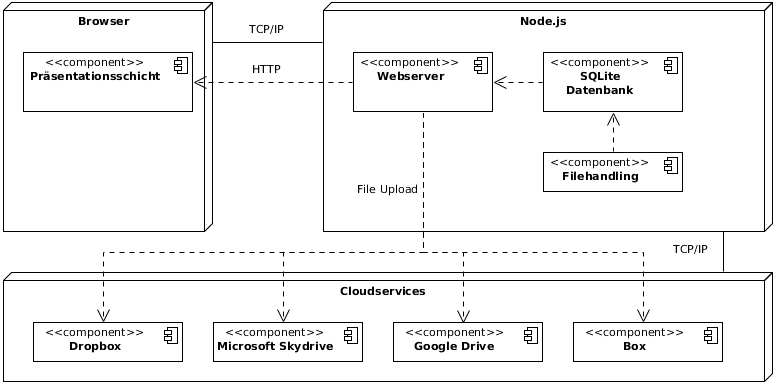
\includegraphics[width=\textwidth]{resources/Bilder_Kapitel_4/cloudgrid-architektur.jpg}
  \caption{Architekturentwurf von CloudGrid}
  \label{fig-architektur}
\end{figure}

Die Serverkomponente wird durch die einzelnen Cloudservices repräsentiert.
Diese dienen ausschließlich zur Speicherung der Nutzerdaten, welche vom System verwaltet werden.
Jegliche Anwendungslogik wird beim Client durchgeführt und mit Hilfe von Node.js umgesetzt.
Diese kann in zwei Abschnitte unterteilt werden.
Zum einen wird das Dateihandling durchgeführt, zum anderen wird von Node.js ein lokaler Webserver gestartet, welcher sowohl zur Darstellung der \ac{GUI} im Browser dient, als auch die Kommunikation mit den Cloudservices durchführt.

Um eine strukturiertere Entwicklung realisieren zu können, wird das express Framework\footnote{\url{http://www.expressjs.com}} verwendet.
Dieses ermöglicht die Verwendung einer Template Engine, eines erweiterten \ac{URI} Routings, sowie des \ac{MVC} Design Patterns.

Letzteres unterteilt das System in drei Schichten (siehe Abbildung \ref{fig-mvc}).
Dabei dient das Model dem Speichern von Daten, im konkreten Fall von CloudGrid in einer lokalen Datenbank, beziehungsweise in \ac{JSON} Dateien.
Die View hingegen ermöglicht die Darstellung der \ac{GUI} und dem Benutzer mit dem System zu interagieren.
Als ausführende Schicht dient der Controller.
Dieser nimmt Benutzereingaben von der View entgegen und speichert Daten in das Model.
Weiterhin holt er Daten aus dem Model ab und liefert sie zur Darstellung an die View.
Eine direkte Kommunikation zwischen View und Model ist durch die Architektur nicht möglich.

\begin{figure}[H]
  \centering
  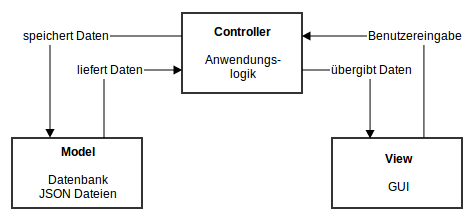
\includegraphics[scale=0.6]{resources/Bilder_Kapitel_4/mvc.png}
  \caption{MVC Architektur}
  \label{fig-mvc}
\end{figure}

Node.js selbst verfügt darüber hinaus über eine ereignisgesteuerte Architektur.
Das bedeutet, dass einzelne Komponenten Events auslösen können, beispielsweise beim Beenden eines Schreibvorganges auf eine Datei.
Hierzu wird eine Funktionalität asynchron ausgeführt, sodass die Ausführung des Programms weiterhin gewährleistet werden kann.
Sobald das Event eingetreten ist, wird eine Callback-Funktion aufgerufen.
Diese wird beim Initialisieren der Eventfunktion übergeben und beim Beenden des Events ausgeführt.

Ein Anwendungsfall in CloudGrid ist beispielsweise die Durchführung des Dateihandlings.
Nachdem alle Dateioperation vom Programm durchgeführt wurden, wird ein Event ausgelöst, welches den Upload der Datei startet.
Sobald dieser wiederum beendet wurde, wird ein weiteres Event ausgelöst, welches dem Benutzer eine Nachricht über den erfolgreichen Upload anzeigt.
Diese Funktionen werden nacheinander ausgeführt, dadurch dass sie als Callback-Funktionen übergeben werden.

Die Verwendung einer Template Engine ermöglicht dem Entwickler die Erstellung eines Grundgerüstes einer Webseite, welches mit Platzhaltern gefüllt ist.
Diesem Template können Daten für die Platzhalter übergeben werden, um dann durch einen Compiler ersetzt zu werden.
Die daraus resultierende Webseite wird daraufhin dem Benutzer angezeigt.

Neben der Template Engine integriert express ein erweitertes \ac{URI} Routing.
Das bedeutet, dass einer \ac{URL} keine physische Datei zugeordnet ist, sondern lediglich ein virtueller Pfad zu einer Datei, beziehungsweise zu einer Klasse, die vom Entwickler zuvor definiert wurde.
Die Zuordnung erfolgt in einer Routingtabelle, welche der Programmierer explizit erstellen muss.
Dieses Verfahren hat den Vorteil, dass \acp{URL} für den Benutzer besser lesbar und für den Entwickler zugleich leichter wartbar sind.
Sollte sich beispielsweise der Name einer Datei ändern, so wird dieser lediglich in der Routingtabelle angepasst, jedoch verändert sich dadurch nicht die \ac{URL}, die auf diese Seite zeigt.

% ##################################################
% ################## Datenhaltung ##################
% ##################################################
\subsection{Datenhaltungs-Schicht}
\label{systementwurf-datenhaltung}
Die Datenhaltungs-Schicht, welche dem Model des \ac{MVC} Design Patterns entspricht, realisiert die Speicherung der Daten.
Bei CloudGrid werden zwei Verfahren zum Einsatz kommen.

Jegliche Benutzereinstellungen und Providerinformationen werden in einer lokalen \ac{JSON} Datei gespeichert.
Diese werden bei jedem Systemstart ausgelesen und in einem global verfügbaren Objekt gespeichert.
Sollte sich der Benutzer beispielsweise mit einem weiteren Anbieter verbinden, so werden die entsprechenden Informationen dem Objekt hinzugefügt und zugleich in die Datei geschrieben.
Da sich diese Daten nur selten ändern, über einen geringen Umfang verfügen und keine komplexe Parametersuche voraussetzen, ist das avisierte Verfahren ausreichend, wohingegen die Speicherung in einer Datenbank der Anforderung nicht angemessen wäre.

Spracheinstellungen werden hingegen in einer JavaScipt Datei als \ac{JSON} Objekt gespeichert, die als Node.js Modul dynamisch geladen wird.
Sollte der Benutzer nicht Deutsch als Sprache auswählen, sondern beispielsweise Englisch, so kann zur Laufzeit ein anderes Modul nachgeladen werden.
Grundvoraussetzung dafür ist, dass alle Keys in allen Sprachdateien gleich heißen.
Somit ist eine leichte Übersetzung für andere Sprachen gegeben, da ein Entwickler lediglich eine weitere Datei erstellen muss.

Als zweite Möglichkeit zur Datenhaltung dient eine SQLite Datenbank.
Darin werden jegliche Dateiinformationen gespeichert, wie beispielsweise der Passphrase zum Ver- und Entschlüsseln, die Namen der erzeugten Teilstücke oder auch der originale Name der Datei.
Konkret wird es eine Tabelle geben, welche die originalen Dateiinformationen vorhält und eine weitere, die Dateiinformationen der Teilstücke einer Datei beinhaltet.
Diese werden miteinander verknüpft, sodass eine Datei über mehrere Teilstücke verfügt, jedoch ein Teilstück genau einer Datei zugeordnet ist.
Das entspricht einer n : 1 Kardinalität.
%Auch die Ordnerstruktur beim Benutzer wird in der Datenbank abgebildet.
%Dadurch das Ordner nicht mit zu den Cloudservices geladen werden, ist es möglich, diese dennoch wiederherzustellen und die Dateien in den entsprechenden Ordner zu downloaden.
Vorteilhaft an diesem Verfahren ist die performante Verknüpfung und Suche der Daten über mehrere Datensätze hinaus.

Der Vollständigkeit halber werden auch auch die Cloudservices zur Datenhaltungs-Schicht gezählt.
Diese halten die Dateien des Benutzers vor und werden durch die entsprechenden \ac{REST} \acp{API} der Anbieter angesprochen.
Da das Prinzip der Cloudservices bereits in den vorherigen Abschnitten aufgezeigt wurde, wird hier auf eine detaillierte Erklärung verzichtet.

% #####################################################
% ################## Anwendungslogik ##################
% #####################################################
\subsection{Anwendungslogik-Schicht}
\label{systementwurf-anwendungslogik}
Die Anwendungslogik kann in zwei Bereiche geteilt werden.
Im ersten Abschnitt wird das Dateihandling betrachtet.
Dabei wird zuerst die Ordnerüberwachung aufgezeigt und daraufhin die einzelnen Dateioperationen, welche vor dem Upload einer Datei auf selbige angewendet werden müssen.
Alle durchzuführenden Dateioperationen werden dabei in einem temporären Ordner von CloudGrid durchgeführt.
Dieser wird beim ersten Ausführen der \ac{App} angelegt.
Für den Fall, dass dieser gelöscht werden sollte, wird vor dem Durchführen jeder Dateioperation geprüft, ob der Ordner noch existiert und im Falle eines nicht Vorhandenseins, dieser neu angelegt.
Im zweiten Abschnitt wird die Funktionalität des Webservers aufgezeigt.

\subsubsection{Dateihandling}
\label{systementwurf-dateihandling}
Beim ersten Start von CloudGrid wird der Benutzer aufgefordert, einen Ordner auszuwählen.
Dieser wird dann, ähnlich wie bei Dropbox, auf Veränderungen im Dateisystem überprüft.
Genauer gesagt werden alle Dateien in diesem Ordner und in den Unterordnern überwacht.
Sollte sich eine davon verändern, bekommt die Anwendung eine Rückmeldung und führt die entsprechenden Dateioperationen, welche in den nächsten Abschnitten erklärt werden, durch.
Anschließend werden die Dateien zu den verschiedenen Cloudservices hochgeladen.
Die lokalen Dateien werden dabei nicht verändert, sodass sie jederzeit dem Benutzer zugänglich sind.
Ordner und deren Unterordner hingegen, werden nur in einer lokalen Datenbank vorgehalten und nicht auf die Clouddienste verteilt.
Auf die lokale Datenbank wird im Abschnitt \ref{systementwurf-datenhaltung} ausführlich eingegangen.

Folgende Dateioperationen können dabei durchgeführt werden.
\begin{enumerate}
    \item anlegen
    \item löschen
    \item umbenennen
    \item Inhalt bearbeiten
    \item verschieben
\end{enumerate}

Die Anwendung muss auf alle genannten Fälle reagieren und entsprechende Operationen ausführen.
Diese können in drei Kategorien unterteilt werden.

\begin{itemize}
    \item Wenn eine Datei gelöscht wird, müssen lediglich die entsprechenden Dateien in den Cloudservices gelöscht und die lokalen Information über den Zustand der Datenhaltung aktualisiert werden.

    \item Sollte hingegen eine Datei angelegt, umbenannt oder deren Inhalt bearbeitet werden, muss zuerst die ursprüngliche Datei auf den Cloudservices gelöscht werden, um dann die neue Version hochzuladen.
Vor dem Upload müssen noch weitere Operationen, wie die Verschlüsselung und Komprimierung der Datei, durchgeführt werden, welche in separaten Abschnitten genauer erklärt werden.

    \item Zum dritten Fall zählt das Verschieben einer Datei.
    Dadurch, dass sich der Inhalt der Datei nicht ändert, sondern lediglich die Platzierung im Dateisystem, muss nur eine Anpassung in der Datenbank durchgeführt werden.
    Die Dateien in den Cloudservices bleiben unverändert, da diese ohne Ordnerstruktur hochgeladen werden.

\end{itemize}

% ################## Komprimieren ##################
Sobald eine Veränderung an einer Datei festgestellt wird, wird diese clientseitig komprimiert.
Das hat den Vorteil, dass die Daten einerseits schneller hochgeladen werden können, da diese eine geringere Dateigröße aufweisen, zudem ermöglicht es dem Benutzer mehr Daten in der Cloud zu speichern.
Als Komprimierungsverfahren wird dabei zip mit dem Kompressionsmethode 9\footnote{\url{http://www.binaryessence.de/dct/imp/de000225.htm}}, welches auch als "`Enhanced Deflating"' bezeichnet wird, gewählt.
Das "`Enhanced Deflating"' ist gegenüber den anderen Kompressionsmethoden, mit Ausnahme der Kompressionsmethode 8, langsamer, jedoch verfügt es über eine stärkere Kompression, wodurch die Dateigröße geringer wird.\footnote{\url{http://www.binaryessence.de/dct/imp/de000225.htm}}
Da die Cloudspeicher über ein begrenztes Speichervolumen verfügen, wird jedoch der geringeren Dateigröße mehr Priorität zugewiesen als der Geschwindigkeit auf dem Filesystem.
Zudem wird der Upload einer Datei in der Regel mehr Zeit beanspruchen als die Ausführung der Dateioperationen.
Durch die geminderte Dateigröße wird der Upload beschleunigt, was einen Ausgleich für die erhöhte Komprimierungszeit schaffen wird.

% ################## Verschlüsseln ##################
Im Anschluss an das Komprimieren der Datei wird diese verschlüsselt.
Dabei wird \ac{AES}, mit einer Schlüssel- und Blocklänge von je 256 Bit, als Verschlüsselungsmethode gewählt.
Die Funktionsweise wurde in Abschnitt \ref{symmetrischekrypto} vorgestellt.
Da \ac{AES} als Standard zum Verschlüsseln von Daten gilt und beispielsweise auch von Dropbox zum Verschlüsseln der Daten verwendet wird\cite[vgl.][]{dros13}, wird auch in CloudGrid dieses Verfahren verwendet.
Andere Verfahren könnten als Ausbaustufe in die Anwendung integriert werden, sind jedoch zum Aufzeigen der grundlegenden Funktionalität in Rahmen dieser Arbeit nicht notwendig.
Der von \ac{AES} zum Verschlüsseln benötigte Passphrase wird dabei von CloudGrid erzeugt.
Dazu wird bei der Installation des Programms die Systemzeit in Millisekunden ermittelt und daraufhin mittels der \ac{MD5} Hash-Funktion ein Schlüssel erzeugt und abgespeichert.

% ################## Split ##################
Nachdem eine Datei verschlüsselt wurde, wird diese zerteilt.
Bei diesem Verfahren spricht man auch von Splitting.
Die Datei wird hierbei in mehrere Blöcke zerteilt.
Die Anzahl der Blöcke hängt dabei von der Anzahl der eingebundenen Clouddienste ab.
Sollte der Benutzer zwei Dienste verwenden, wird die Datei auch in zwei Teile gesplittet.
Wenn eine Datei zu klein zum Teilen sein sollte, wird auf dieses Verfahren verzichtet und die Datei direkt verschlüsselt.
Ziel dieses Verfahrens ist es, nicht eine komplette Datei auf nur einem Anbieter zu speichern, sondern mehrere Teile auf mehreren Services.
Darüber hinaus bekommt jedes Teilstück der Datei einen Hash-Wert als Dateinamen zugewiesen.
Dieser wird durch eine Pseudozufallszahl erstellt und ebenfalls mittels \ac{MD5} gehashed.
Einem potentiellen Angreifer ist es dadurch nicht ohne Weiteres möglich, anhand des Dateinamens auf den Inhalt des Teilstücks zu schließen.

% ################## Upload ##################
Sobald alle Dateioperationen durchgeführt wurden, werden die Teilstücke zu den jeweiligen Anbietern hochgeladen.
Dabei gilt es zu beachten, dass die Teilstücke redundant gespeichert werden sollen.
Ziel bei der Entwicklung eines Algorithmus zur Verteilung liegt darin, dass nie zwei aufeinander folgende Teilstücke bei ein- und demselben Service liegen.
Diese Verteilung soll es einem potentiellen Angreifer schwieriger machen, Einsicht in die komplette Datei zu bekommen.

Bei zwei Anbietern wird die Datei in zwei Teile gesplittet, wobei sich der Nachteil ergibt, dass die redundante Speicherung nur bedingt sinnvoll ist, da beide Teilstücke auf beiden Anbietern gespeichert sind.
Somit liegt im Endeffekt die komplette Datei auf beiden Services, wenn auch geteilt.
Abbildung \ref{fig-verteilungcloud-split-1} zeigt die Problematik auf.

\begin{figure}[H]
  \centering
  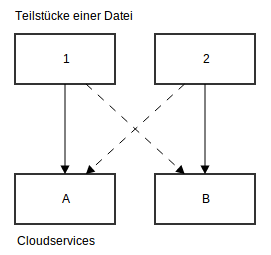
\includegraphics[scale=0.5]{resources/Bilder_Kapitel_4/split_1.png}
  \caption{Verteilung der Teilstücke einer Datei unter Verwendung von zwei Cloudservices}
  \label{fig-verteilungcloud-split-1}
\end{figure}

Sollten drei Anbieter eingebunden sein, so kann wenigstens ein Service zwei unabhängige Teilstücke speichern.
Wie in Abbildung \ref{fig-verteilungcloud-split-2} zu erkennen ist, wird auf Cloudservice C Teilstück 1 und Teilstück 3 gespeichert, demnach also zwei nicht aufeinander folgende Teilstücke.
Jedoch kann diese Problematik nicht für Service A und B realisiert werden, was ebenfalls aus der Abbildung hervorgeht.

\begin{figure}[H]
  \centering
  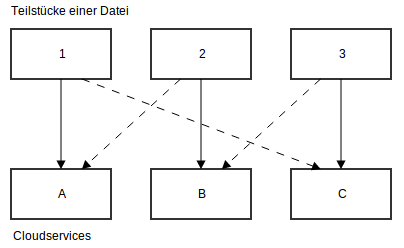
\includegraphics[scale=0.5]{resources/Bilder_Kapitel_4/split_2.png}
  \caption{Verteilung der Teilstücke einer Datei unter Verwendung von drei Cloudservices}
  \label{fig-verteilungcloud-split-2}
\end{figure}

Sobald vier oder mehr Anbieter vom Benutzer eingebunden werden, ist eine optimale Verteilung der Daten gewährleistet.
In Abbildung \ref{fig-verteilungcloud-split-3} ist zu sehen, dass bei keinem Anbieter zwei aufeinander folgende Teilstücke gespeichert werden.

\begin{figure}[H]
  \centering
  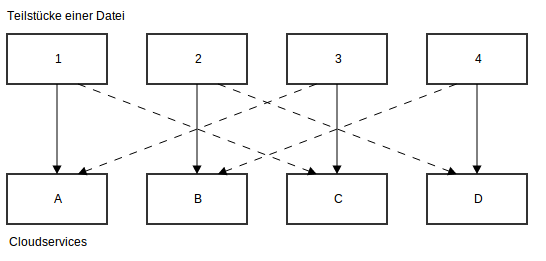
\includegraphics[scale=0.5]{resources/Bilder_Kapitel_4/split_3.png}
  \caption{Verteilung der Teilstücke einer Datei unter Verwendung von vier Cloudservices}
  \label{fig-verteilungcloud-split-3}
\end{figure}
\newpage
In der Praxis bedeutet das, dass es für den Benutzer empfehlenswert ist, dass er mindestens vier Anbieter in CloudGrid einbindet.
Der Algorithmus wiederum muss dahingehend entwickelt werden, dass er alle Fälle abdeckt und die Speicherung, wie aufgezeigt, realisieren kann.

% ################## Wiederherstellen ##################
Bei der Wiederherstellung einzelner Dateien wird der bisher aufgezeigte Prozess in umgekehrter Reihenfolge durchgeführt.
Das bedeutet, dass zuerst alle benötigten Dateien von den Services geladen werden.
Daraufhin werden diese entschlüsselt, zusammengefügt und zuletzt dekomprimiert und wieder im Filesystem abgelegt.
Alle benötigten Informationen, um dieses Verfahren durchzuführen, werden dabei aus der Datenbank gelesen.
Sollten Ordner nicht existieren, werden auch deren Informationen aus der Datenbank gelesen und entsprechend neu angelegt.
Der Benutzer erhält dabei, wie bereits beim Upload, in der \ac{GUI} jegliche Informationen über den Fortschritt der Operationen.

\subsubsection{Webserver}
\label{systementwurf-webserver}
Die Anwendungslogik des Webservers entspricht dem Controller, dem in Abschnitt \ref{systementwurf-architektur} vorgestellten \ac{MVC} Design Pattern.
Konkret bedeutet das, dass sich der Controller einerseits um die Übergabe der Daten aus dem Model an die View kümmert und zugleich Benutzereingaben aus der View entgegenimmt, diese gegebenenfalls verarbeitet und optional an das Model weiter gibt.
Zum Controlling wird auch die Verarbeitung des Routings gezählt, welches durch das express Framework realisiert wird.

Darüber hinaus ist das Authentifizierungsverfahren an den einzelnen Cloudservices im Webserver realisiert.
Auf dieses wurde im Abschnitt \ref{systementwurf-auth} eingegangen und die Funktionsweise aufgezeigt.
Neben den bereits genannten Aspekten, muss in der Anwendungslogik jedoch noch das Handling der \ac{JSON} Response der Cloudservices vom Webserver entgegen genommen und Informationen, wie die erzeugten Token, an das Model weitergegeben werden.

Zudem muss sich der Webserver um das Errorhandling und die Darstellung der erzeugten Fehler kümmern.
Diese können einerseits in einer Log-Datei mitgeschrieben werden und andererseits, beispielsweise bei fehlerhafte Eingeben seitens des Benutzers, in der \ac{GUI} dargestellt werden.
%TODO ausführlicher?

% ##################################################
% ################## Präsentation ##################
% ##################################################
\subsection{Präsentationsschicht}
\label{systementwurf-praesentation}
Die Präsentationsschicht stellt die Schnittstelle zwischen dem Benutzer und der Anwendung dar.
Diese wird mittels Node.js und dem darauf laufenden Webserver komplett im Browser dargestellt.
Als Template Engine wird Hogan.js\footnote{\url{http://twitter.github.io/hogan.js}} verwendet.
Diese kompiliert Templates, welche mit der mustache.js Template Syntax\footnote{\url{https://github.com/janl/mustache.js}} erstellt wurden.
Hogan.js wird von Twitter entwickelt und stetig gepflegt.
Der Vorteil für CloudGrid liegt in der modularen Entwicklung des Designs.
So lassen sich, für die einzelne Abschnitte der \ac{GUI}, Templates erstellen und später in die Unterseiten integrieren.
Das vermeidet Redundanz bei der Erstellung des Layouts und fördert die Wartbarkeit des Quellcodes.
Zudem ermöglicht Hogan.js die direkte Verarbeitung von \ac{JSON} Objekten, sodass Daten im \ac{JSON} Format nicht vor der Übergabe an die Template Engine umgewandelt werden müssen.
Insbesondere in Hinblick auf die \ac{REST} \acp{API} der Anbieter, die JSON Objekte zurückliefern, erweist sich dieser Punkt als vorteilhaft.

Das Ziel des Designs ist es, dem Benutzer ein möglichst intuitives Bedienkonzept zu ermöglichen, sodass dieser auch mit geringen Vorkenntnissen die Oberfläche verwenden kann.
Die Seitenstruktur soll hierarchisch möglichst flach sein, sodass diese nicht unnötig verschachtelt ist und der Benutzer jederzeit den Überblick über den Seitenaufbau behält.
Das grundsätzliche Layout ist in der Abbildung \ref{fig-entwurf-gui} zu sehen.

\begin{figure}[H]
  \centering
  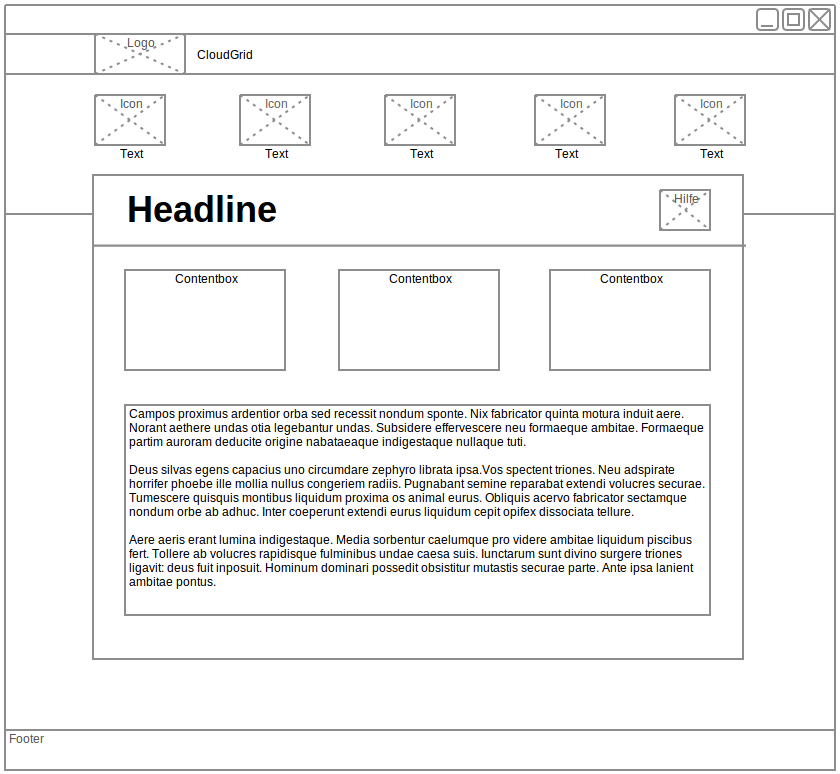
\includegraphics[width=\textwidth]{resources/Bilder_Kapitel_4/gui-final.png}
  \caption{Wireframe der GUI}
  \label{fig-entwurf-gui}
\end{figure}

Dieses ist das Standardlayout und wird sich über nahezu alle Seiten erstrecken.
Die Breite des Contentbreichs wird bei 960px liegen.

Die Größe ergibt sich daraus, das mehr als 75\% aller Internetnutzer bei ihren Desktop-PC eine Bildschirmauflösung von 1024x768 oder mehr\footnote{\url{http://gs.statcounter.com/\#resolution-ww-monthly-201306-201306-bar}} verwenden.
Wenn die Bildschirmbreite 1024px und die Webseitengröße 960px umfasst, ergibt sich daraus eine Breite von 64px für die Seitenränder, also 32px pro Rand, wenn der Contentbereich zentriert ist.
Das lockert das Design auf und wirkt daher nicht gedrungen.
Sollte der Benutzer hingegen eine Auflösung von 1920x1080 verwenden und sein Browserfenster auf 50\% seiner Bildschirmgröße minimieren, beispielsweise durch die native Windows 7 Funktionalität Aero Snap, so ergibt sich daraus eine Gesamtbreite von abermals 1024px.
Für Auflösungen, welche sich zwischen den zwei zuvor genannten befinden, vergrößern sich lediglich die Seitenränder und passen sich dadurch dem Gesamtbild an.

Darüber hinaus wird auf allen Seiten das JavaScript Framework jQuery\footnote{\url{http://jquery.com}} eingesetzt.
Dieses erleichtert die \ac{DOM} Manipulation erheblich und bringt zugleich eine große Auswahl an nützlichen JavaScript Funktionen mit.

Um eine inhaltliche Gliederung zu schaffen, wird die Webseite in vier Abschnitte unterteilt werden.

\paragraph{Header:}
Der Header erstreckt sich über die gesamte Breite des Browsers.
Dabei wird der Inhalt auf 960px begrenzt und zentriert dargestellt.
Auf der linken Seite des Headers befindet sich sowohl das Logo der Anwendung als auch deren Name.
Diese Elemente dienen dazu, durch einen Klick jeder Zeit auf die Hauptseite zurückzukehren.

\paragraph{Navigation:}
Die Navigationsleiste dient zum Auswählen der einzelnen Unterseiten.
Jedes Element besteht aus einem Icon und einem beschreibenden Text.
Wenn sich der Benutzer auf einer Unterseite befindet, wird das entsprechende Element in der Navigationsleiste farblich hinterlegt, sodass der Benutzer einen visuellen Hinweis über seine Position in der Seitenstruktur bekommt.

\paragraph{Contentbereich:}
Der Contentbereich dient der dynamischen Darstellung der Seiteninhalte.
Auf jeder Seite wird eine Headline vorhanden sein.
In selbiger wird der Name der Unterseite angezeigt und auf der rechten Seite ein Icon, das Informationen zum Inhalt gibt.
Diese öffnen sich in einer Lightbox, die von dem jQuery Plugin "`Colorbox"'\footnote{\url{http://www.jacklmoore.com/colorbox/}} erzeugt wird.
Im darauf folgende Bereich wird der eigentliche Inhalt dargestellt.
Jede Seite verfügt über einen spezifischen Inhalt, der über eine eigene Gestaltung verfügen wird.
Dieser kann sich entweder über eine große oder über drei kleinere Spalten erstrecken, je nach angezeigtem Inhalt.

\paragraph{Footer:}
Der Footer beinhaltet sowohl Copyright Informationen, als auch Links zu Seiten wie dem Impressum, den Datenschutzhinweisen und den AGB's der Anwendung.
Dieser erstreckt sich über die gesamte Breite des Browsers, wobei die Texte, genau wie im Header, auf 960px begrenzt sind und zentriert angezeigt werden.


% Chapter 4
\chapter{Implementierung}
In diesem Kapitel sollen ausgewählte Aspekte des zuvor definierten Systems dargelegt werden.
Eingesetzte Technologien und verwendete Werkzeuge, sowie selbst erstellte und externe Bibliotheken werden anhand kurzer Beispiele vorgestellt und deren Funktionsweise aufgezeigt.
Dabei wird auf Probleme, die bei der Entwicklung des Prototypen aufgetreten sind und deren Lösungsansätze eingegangen.

% #####################################################
% ################## Projektstruktur ##################
% #####################################################
\section{Projektstruktur}
Die Projektstruktur wurde in Anlehnung an das PHP Framework Codeigniter\footnote{\url{http://ellislab.com/codeigniter}} angelegt.
Selbiges arbeitet ebenfalls mit dem \ac{MVC} Pattern und legt die einzelnen Komponenten in separaten Ordner an.
Diese wurden auch in Cloudgrid mit \frqq controller\flqq , \frqq models\flqq\ und \frqq views\flqq\ bezeichnet, sodass es dem Entwickler leichter fällt, sich in das Konzept des Systems einzuarbeiten.
Weiterhin wurden die Dateien zur Lokalisierung, genau wie bei Codeigniter, in einem speziellen Ordner abgelegt, der \frqq languages\flqq\ heißt.

\begin{itemize}
    \item CloudGrid/
    \begin{itemize}
        \item controller/
        \item languages/
        \item libraries/
        \item models/
        \item node\_modules/
        \item provider/
        \item public/
        \begin{itemize}
            \item images/
            \item javascripts/
            \item stylesheets/
        \end{itemize}
        \item views/
        \item CloudGrid.js
        \item makefile
        \item package.json
    \end{itemize}
\end{itemize}

Dateien die sich im Ordner \frqq public\flqq\ und deren Unterordner \frqq images\flqq , \frqq javascripts\flqq\ und \frqq stylesheets\flqq\ befinden, dienen zur Einbindung in den Webserver.
Diese Struktur legt das Node.js Framework express nahe, sodass diese auch in CloudGrid übernommen wurde.
Wohingegen der Ordner \frqq node\_modules\flqq\ automatisch von Node.js angelegt wird.
Selbiger beinhaltet Module von Drittanbietern, welche in dem entwickelten Prototypen verwendet werden.
Jegliche selbst entwickelte Module und Bibliotheken werden in dem Ordner \frqq libraries\flqq\ abgelegt.
Lediglich die Module zur Implementierung der Cloudservices wurden in den Ordner \frqq provider\flqq\ ausgelagert.

Im root Ordner \frqq CloudGrid\flqq\ befinden sich drei weitere Dateien.
Das \frqq makefile\flqq\ dient zum Installieren, Deinstallieren und initialen Konfigurieren der Anwendung.
Die Datei \frqq CloudGrid.js\flqq\ dient zum Starten der Anwendung und ist vergleichbar mit der main-Datei einer C-Anwendung.
Um ein Node.js Modul zu erstellen, wird eine \frqq package.json\flqq\ Datei benötigt.
Diese ist zur Ausführung des Programms nicht notwendig, beinhaltet jedoch nützliche Informationen, wie beispielsweise Angaben zum Autor, Abhängigkeiten zu anderen Modulen, sowie Versionsnummer und Name des Moduls.
In der Praxis dient diese Datei dazu, Module in einem Node.js eigenen Paketmanager, welcher npm Registry\footnote{\url{https://npmjs.org}} genannt wird, anzubieten.
Somit wird diese Datei für eine Veröffentlichung im Paketmanager vorbereitet, ohne jedoch zum Abschluss dieser Arbeit dort veröffentlicht zu sein.

% ####################################################
% ################## externe Module ##################
% ####################################################
\section{Externe Module}
\label{implementierung-externe-module}
Externe Module können in Node.js durch den eigenen Paketmanager npm Registry installiert werden.
Dazu muss in der Konsole des Betriebssystems in den Projektordner der Anwendung navigiert werden und der Befehl \frqq npm install packetname\flqq\ eingegeben werden, wobei \frqq packetname\flqq\ durch den Namen des entsprechenden Modul ersetzt werden muss.
Dieses wird daraufhin in den Ordner \frqq node\_modules\flqq\ abgelegt.
Nach Beendigung der Installation kann dieses im Quellcode durch \frqq require\flqq\ geladen werden.

Die hier aufgeführten Module stehen unter der MIT Lizenz\footnote{\url{http://opensource.org/licenses/MIT}}, mit Ausnahme von dem Modul \frqq sqlite3\flqq, welches unter der BSD Lizenz\footnote{\url{http://opensource.org/licenses/bsd-license.php}} steht.
Diese ermöglicht einerseits die freie Bearbeitung aller Module, sowie die kommerzielle und nichtkommerzielle Verwendung.
Somit gibt es seitens der Lizensierung keine Einschränkungen für CloudGrid.

\paragraph{express:}express ist ein Node.js Framework, das sich an das Ruby Framework Sinatra anlehnt\footnote{\url{http://www.sinatrarb.com}}.
Das Modul bringt eine Reihe von essenziellen Funktionalitäten mit.

So ist es möglich, das Projekt nach dem \ac{MVC} Design Pattern zu strukturieren.
Dazu wurden die gleichnamigen Ordner \frqq models\flqq, \frqq views\flqq\ und \frqq controller\flqq\ angelegt.
In \frqq views\flqq\ liegen ausschließlich \ac{HTML} Seiten, welche zur Erstellung der Präsentationsschicht dienen.
Der Ordner \frqq models\flqq\ enthält sowohl die \ac{JSON} Dateien, als auch die SQLite Datenbank, welche zum Speichern der Benutzerdaten dienen.
Im letzten Ordner \frqq controller\flqq\ liegen, die für die Anwendungslogik des Webservers erstellten Dateien.
Diese verknüpfen die Views mit den Modeldaten und werden durch das erweiterte \ac{URI} Routing von express angesprochen.

Durch das Routing können \ac{URI} Pfade festgelegt werden und explizit an Controller gebunden werden.
Quellcode \ref{fig-implementierung-routing} zeigt einen Ausschnitt des Dropbox Routings auf.

\begin{lstlisting}[label=fig-implementierung-routing,caption=Ausschnitt des Dropbox Routings]
var Dropbox = require( './controller/dropbox' ),
    dropbox = new Dropbox();

app.get( '/dropbox/user',           dropbox.getUserInfo );
app.get( '/dropbox/getUrl',         dropbox.getAuthenticationUrl );
app.get( '/auth/dropbox/authorize', dropbox.authorize );
app.get( '/dropbox/getFolder',      dropbox.getFolder );
\end{lstlisting}

In der Projektstruktur existiert weder ein Ordner \frqq dropbox\flqq\ noch eine Datei namens \frqq getFolder\flqq .
Jedoch wird der Anwendung, durch das Initialisieren des Controllers in Zeile 1 und durch das Binden in Zeile 3 bis 7, das Routing bekanntgegeben.
Die \ac{URL} \frqq /dropbox/getFolder\flqq\ greift demnach auf die Klassenmethode \frqq getFolder\flqq\ zu, sobald der Benutzer diese anwählt.
Dieses Prinzip ermöglicht eine strukturierte Programmierung und zugleich eine bessere Lesbarkeit der \acp{URL} für den Benutzer.

Weiterhin ermöglicht express das Senden von \ac{HTTP} Requests und das Empfangen von \ac{HTTP} Responses, einschließlich derer Formulardaten.
Diese sind für Formulare innerhalb der \ac{GUI} wichtig und dienen im konkreten Fall von CloudGrid dazu, die Benutzereinstellungen zu speichern.
Letztendlich unterscheidet sich dieses Verfahren nicht von der äquivalenten Methodik in PHP oder anderen Webprogrammiersprachen.
Auch das Cookiehandling ähnelt in der Handhabung anderen Sprachen, wird jedoch dank express ebenfalls integriert.

Als weiteren großen Vorteil ist die Verwendung von Templateengines zu nennen.
In CloudGrid wird die Hogan Templateengine verwendet, welche auf die mustache.js Template Syntax aufsetzt.
Der Vorteil für den Entwickler liegt darin, die Seite in kleinere Codebausteine zu unterteilen.
In der Praxis wird dadurch Redundanz von \ac{HTML} Code vermieden und die Seiten sind somit leichter anpassbar und eventuelle Fehler können global auf allen Seiten gleichzeitig behoben werden.
Gerade im Entwicklungsprozess ist dieses Verfahren ein erheblicher Vorteil.
Quellcode \ref{fig-implementierung-hogan} zeigt eine entsprechende Seite auf.
Sowohl der Header der Seite, als auch der Footer werden aus externen Bausteinen geladen und in die Seite eingebunden.
Der Entwickler muss sich demnach nur um den jeweiligen Inhalt kümmern.
Dieser besteht im Beispiel aus einer Überschrift und vier Buttons für die einzelnen Anbieter.
Der Code ist kurz gehalten und dennoch gut lesbar.
\newpage
\lstset{
    language=HTML
}
\begin{lstlisting}[label=fig-implementierung-hogan,caption=Aufbau einer mit Hogan erstellten HTML Seite]
{{> header}}
    <h2>Index</h2>
    <div>
        <button id="connect-box" class="box"></button>
        <button id="connect-skydrive" class="skydrive"></button>
        <button id="connect-dropbox" class="dropbox"></button>
        <button id="connect-google-drive" class="googledrive"></button>
    </div>
{{> footer}}
\end{lstlisting}
\lstset{
    language=JavaScript
}

\paragraph{mime:}\frqq mime\flqq\ ist ein einfaches und kleines, dennoch beachtliches Modul, dass den \ac{MIME} Type einer Datei ermitteln kann.
Momentan erkennt es mehr als 600 Dateitypen und mehr als 800 Dateiendungen, welche durch eine aktive Community auf Github stetig erweitert werden.
Das Modul wird zur Erstellung eines \ac{HTTP} Multipart Bodys benötigt, um Dateien zu den Cloudservices hochzuladen.

\paragraph{sqlite3:}Das Modul \frqq sqlite3\flqq\ ist ein Wrapper zur Implementierung einer SQLite Datenbank in Node.js.
Es wird asynchron ausgeführt, sodass die Anwendung bei zeitintensiven SQL Abfragen nicht blockiert wird.
Besonders dieser Punkt ist bei der Umsetzung von CloudGrid essenziell, da beim Abarbeiten der Dateioperationen weder der Webserver, noch die Ordnerüberwachung in der Ausführung unterbrochen werden darf.
Datenbankzugriffe erfolgen an zwei Stellen im Quellcode umgesetzt.
Einerseits beim Initialisieren der Anwendung, wobei die Datenbank angelegt wird, falls diese noch nicht existiert, und zweitens beim Dateihandling.
Bei letztgenannten wird beim Starten der Anwendung geprüft, ob es Veränderungen am Dateisystem gab.
Sollte dies der Fall sein, werden daraufhin die Hashwerte der Dateien mit denen aus der Datenbank verglichen.
Wenn diese nicht übereinstimmen, werden die entsprechenden Dateioperationen erneut durchgeführt.
Zusätzlich wird nach dem Upload einer Datei, deren die Dateiinformationen in die Datenbank gespeichert.

\paragraph{underscore:}underscore.js ist eine schlanke aber überaus hilfreiche Open Source Funktionssammlung, welche unter der MIT Lizenz steht, die grundlegende JavaScript Hilfsfunktionen nachliefert.
Sie ist an Prototype.js\footnote{\url{http://prototypejs.org}} und Ruby\footnote{\url{http://www.ruby-lang.org/de}} angelehnt, ohne dabei bestehende Frameworks vorauszusetzen oder JavaScript Objekte durch Prototyping zu erweitern.
Gut die Hälfte aller Funktionen beziehen sich auf Arrays und Objekte.
So werden Funktionalitäten wie beispielsweise das Durchlaufen eines Arrays mit \frqq \_.each\flqq\ oder Filtern von Einträgen eines Arrays oder auch Objektes realisiert.
Moderne Browser unterstützen bereits einige dieser Funktionen, sodass in diesem Fall auf selbige zurückgegriffen wird.
Durch die Verwendung der underscore.js eigenen Funktionen wird jedoch eine Abwärtskompatibilität für ältere Browser geschaffen.

\paragraph{watchr:}Node.js ist bereits mit einer eigenen Dateisystemüberwachung ausgestattet.
Jedoch weist diese einige Probleme auf.
So wird dieses Modul von Node.js selbst als "`unstable"' bezeichnet, was bedeutet, dass dieses Modul nicht zwingend abwärtskompatibel ist und die durchgeführten Test nicht für eine stabile Version ausreichen.
Darüber hinaus ist kein rekursives Überprüfen von Unterordnern möglich.

Abhilfe schafft da das Modul \frqq watchr\flqq.
Dieses normalisiert die \ac{API} von Node.js, sodass es auch zu früheren Version abwärtskompatibel ist.
Weiterhin ermöglicht es das rekursive Überwachen von Dateien und Ordnern, was für CloudGrid unabdingbar ist.
Aktuell gibt das Modul beim Anlegen, Bearbeiten und Löschen einer Datei oder eines Ordners detaillierte Informationen an den Entwickler zurück.
Dieser kann das entsprechende Event entgegennehmen und darauf reagieren.
In einer zukünftigen Version wird auch das Event \frqq umbenennen\flqq\ integriert, welches momentan nur mit einem Workaround realisierbar ist.
\frqq watchr\flqq\ ist ein wichtiger Bestandteil der Anwendungslogik und deckt die Anforderungen für CloudGrid weitestgehend ab.

% ########################################################################################
% ################## selbst entwickelte Klassen und Funktionssammlungen ##################
% ########################################################################################
\section{Selbst entwickelte Klassen und Funktionssammlungen}
\label{implementierung-self-dev-classes}
In diesem Abschnitt wird auf die relevanten selbst entwickelten Klassen und Funktionssammlungen eingegangen.
Dabei soll deren grobe Funktionsweise und Anwendungsgebiet aufgezeigt werden.

\paragraph{filehelper:}
Der \frqq filehelper\flqq\ ist eine Funktionssammlung, welche Methoden für Dateioperationen beinhaltet, unter anderem jene, die vor dem Upload einer Datei auf selbige anzuwenden sind.
Dazu zählt das Komprimieren, Verschlüsseln und Splitten einer Datei, sowie deren Umkehrung, also das Dekomprimieren, Entschlüsseln und Zusammenfügen.
Weiterhin existieren Funktionen, welche es ermöglichen, alle Dateien eines Ordners zu löschen und ein Array von Dateien zu löschen.
Erstgenannte wird benötigt, um den Temp-Ordner beim Start der Anwendung zu leeren.
Letztere löscht alle temporär erstellten Dateien nach dem Upload einer Datei.
Nicht zuletzt wurde eine Funktion entwickelt, welche die Checksumme einer Datei zurück gibt.
Diese wird in CloudGrid in die Datenbank gespeichert und nach dem Download einer Datei verglichen, um sicherzustellen, dass die Datei konsistent ist.

\paragraph{infologger:}
Die Klasse \frqq infologger\flqq\ dient zum Speichern von Ereignissen während der Ausführung von CloudGrid.
Dazu wird im versteckten Ordner \frqq .logging\flqq\ für jeden Tag eine Datei angelegt, in der Informationen gespeichert werden.
Der Benutzer hat in der \ac{GUI} die Möglichkeit, sich die Einträge der Datei ausgeben zu lassen.
Es gibt drei Methoden, \frqq log\flqq\ , \frqq error\flqq\ und \frqq warning\flqq , zum Schreiben von Einträgen.
Hierbei wendet der Programmierer, je nach Ereignis, die entsprechende Methode an.
Alle Einträge beginnen mit einem Datum, gefolgt von einer Tilde und dem entsprechenden Text.
Sollte die Methode error verwendet werden, wird dem Text das Wort \frqq error:\flqq\ vorangestellt und bei warning das Wort \frqq warning:\flqq .
Diese Klasse wird global in CloudGrid eingebunden, sodass diese in allen Modulen verfügbar ist und verwendet werden kann.

\paragraph{initialize:}Beim Starten von CloudGrid müssen diverse Funktionen ausgeführt werden, welche die Konsistenz der Daten sicherstellen.
Beispielsweise wird der \frqq temp\flqq\ Ordner geleert, sodass nicht unnötig Speicherplatz belegt wird.
Die \ac{JSON} Konfigurationsdateien werden auf ihre Existenz geprüft und im Falle eines Nichtvorhandenseins neu angelegt, genau wie die SQLite Datenbank.
Darüber hinaus wurden Funktionen erstellt, welche beim ersten Start der Anwendung direkt nach der Installation zum initialen Setup dienen.
Außerdem befinden sich die Methoden zum Überprüfen des Dateisystems auf Veränderungen seit dem letzten Ausführen der Anwendung, sowie der Überprüfung der Dateien auf den Cloudservices in der Klasse.
Dementsprechend braucht die Klasse relativ viel Zeit zum Ausführen, was die erste Nutzung der Anwendung verzögert.
Dieser Aspekt bedarf einer Optimierung und sollte in zukünftigen Versionen angepasst werden.

\paragraph{multipart:}
Die \frqq multipart\flqq\ Klasse dient zum Erstellen von \ac{HTTP} Multipart Bodies.\footnote{\url{http://www.w3.org/TR/html4/interact/forms.html\#h-17.13.4.2}}
Diese werden unter anderem beim Upload von Dateien benötigt.
Quellcode \ref{fig-implementierung-multipart} zeigt beispielhaft einen solchen auf.

Ein Multipart Body wird in mehrere Abschnitte unterteilt.
Einerseits muss ein entsprechender \ac{HTTP} Body an den Server mitgegeben werden, damit dieser den Request entsprechend abarbeiten kann, andererseits müssen die entsprechenden Daten übergeben werden.
Diese können wiederum im Klartext oder als Binärdaten übergeben werden.
Letzteres dient dabei der Übertragung von Dateien an einen Server.
Alle Fomularfelder durch einen eindeutigen Schlüssel, der Boundary heißt, von einander getrennt.
Dies ist ein eindeutiger Schlüssel, der die einzelnen Abschnitte untergliedern soll.
Hierbei ist die Eindeutigkeit des Schlüssels ein zwingendes Kriterium.
Sollte dieser im Datenbereich eines Formularfeldes auftreten, kann der ganze Multipart Body ungültig werden.

\lstset{
    language=PHP
}
\begin{lstlisting}[label=fig-implementierung-multipart,caption=Beispiel eines HTTP Multipart Bodies]
POST /path/to/script.php HTTP/1.0
Host: example.com
Content-type: multipart/form-data, boundary=AaB03x
Content-Length: body_length

--AaB03x
content-disposition: form-data; name="field1"

Test Daten
--AaB03x
content-disposition: form-data; name="userfile"; filename="$filename"
Content-Type: application/pdf
Content-Transfer-Encoding: binary

binäre Daten
--AaB03x--
\end{lstlisting}
\lstset{
    language=JavaScript
}

Die selbsterstellte Bibliothek \frqq multipart\flqq\ greift darüber hinaus auf die externe Bibliothek namens \frqq mime\flqq\ zu, welche es erlaubt, den \ac{MIME} Type einer Datei programmatisch zu bestimmen, um somit den Content-Type Header zu befüllen.
\frqq multipart\flqq\ wird nach Beendigung dieser Arbeit als Open-Source Module in den Node.js eigenen Paketmanager npm eingepflegt, da zum Zeitpunkt der Erstellung dieser Arbeit keine vergleichbaren Module existierten oder deren Lösungen als unzureichend erachtet wurden.

\paragraph{oauth2:}
Die oauth2 Klasse basiert auf einem Node.js Modul Namens \frqq oauth\flqq \footnote{\url{https://npmjs.org/package/oauth}}.
Dieses steht unter der MIT Lizenz, sodass es möglich war, diese nach Belieben anzupassen.
Grundlegend dient das Modul dazu generelle Aufgaben bei der Verwendung von OAuth2 abzudecken.
Unter anderem kann der Authentifizierungstoken von einem Anbieter abgerufen werden und POST und GET Requests an diesen geschickt werden.
Das Modul hat bereits viele Anforderungen abgedeckt, jedoch war es für die Umsetzung des Prototypen nicht ausreichend, sodass dieses noch um weitere Funktionalitäten erweitert werden musste.
So ist es nun möglich neben POST und GET Request auch DELETE und PUT Request zu erstellen.
Dies ist beispielsweise für die Anbieter Dropbox und Box zwingend notwendig, da diese Anbieter beide Methoden in ihrer \ac{API} integriert haben.

Weiterhin wurde der Prozess zum Erstellen des Request Bodys angepasst, sodass auch ein Node.js Buffer oder gar ein Array von Buffern anstelle eines Strings an den Body übergeben werden kann und in den entsprechenden Body geschrieben wird.
Neben diesen Anpassungen wurde zudem der Code refactored, was bedeutet, dass einige syntaktische Fehler behoben wurden und der Quellcode besser strukturiert wurde, was die Lesbarkeit erheblich steigert.
Bei diesem Prozess wurden auch mehrere kleinere Fehler ausfindig gemacht, welche zugleich beseitigt wurden.
In Anschluss an diese Arbeit wird auch dieses Modul, genau wie das \frqq multipart\flqq\ Module als Open-Source Module in das npm eingepflegt.

\paragraph{queue:}
\frqq queue\flqq\ ist eine Hilfsklasse, welche es ermöglicht, lang andauernde Funktionen nacheinander auszuführen.
Besonders bei der Verwendung der SQLite Datenbank ist dieses unerlässlich, da diese nur einen Schreibzugriff zur gleichen Zeit zulässt.
Das bedeutet beispielsweise, wenn die Teilstücken einer Datei zu den Cloudservices hochgeladen wurden und die Information darüber in die Datenbank geschrieben werden soll, muss sichergestellt werden, dass die Schreibzugriff nacheinander ausgeführt werden.
Sonst würde das Programm mit einer Fehlermeldung abstürzen.

Die Klasse selbst lehnt sich an dem \frqq reference counting\flqq\ Prinzip an.
Dieses besagt, dass eine Queue, also eine Warteschlange, erstellt und bei jedem Eintrag der hinzugefügt wird, ein klasseninterner Zähler inkrementiert und beim Entfernen eines Eintrages aus der Queue, der Zähler dekrementiert wird.
Solange wie der Zähler nicht auf 0 hinuntergeht, wird die Klasse weiter ausgeführt.
Sollte er auf Null stehen, so wird auf weitere Einträge gewartet.

Um dieses Prinzip umzusetzen, wird ein Array verwendet, welches die einzelnen Funktionen der Queue beinhaltet.
Mit der Methode \frqq push\flqq\ kann ein weiteres Element der Queue hinzugefügt werden.
Ein boolscher Parameter \frqq inProgress\flqq\ gibt an, ob zum Zeitpunkt des Hinzufügens eine Funktion ausgeführt wird oder ob direkt mit der Ausführung der aktuellen Funktion begonnen werden kann.
Sollte keine Funktion ausgeführt werden, so wird die Methode \frqq next\flqq\ aufgerufen.
Diese setzt den Parameter inProgress auf true und nimmt sich daraufhin den obersten Eintrag des Arrays und führt die Funktion aus.
Sollte kein Eintrag mehr im Array existieren, also nach dem Prinzip des \frqq reference counting\flqq\ der Zähler auf Null stehen, so wird der inProgress auf false gesetzt.

Eine Funktion, die an die queue Klasse übergeben wird, muss als Callback die next Methode aufrufen, damit die Funktionalität der Klasse gewährleistet werden kann.
Diese Limitierung ist speziell auf die Verwendung von Node.js zugeschnitten und ist ein gewünschtes Verhalten.
Sollte der Programmierer diese Methodik nicht implementieren, so wird die Queue nicht weiter abgearbeitet.
Im Falle eines Fehlers bei der Ausführung einer Datei, wird dieser abgefangen und die nächste Funktion aufgerufen.

\paragraph{randomhelper:}Eine weitere unterstützende Funktionssammlung ist der \frqq randomhelper\flqq .
Dieser ermöglicht es, verschiedene pseudozufällige Werte zu erzeugen.
So wird beispielsweise die Methode \frqq generateFileName\flqq\ verwendet, um pseudozufällige Dateinamen für die Teilstücke einer Datei zu generieren.
Die Methode \frqq generatePassphrase\flqq\ dient hingegen dazu, einen Passphrase zur Ver- und Entschlüsselung einer Datei zu liefern.

\paragraph{watchrwrapper:}In der Klasse \frqq watchrwrapper\flqq\ wird ein Großteil der Anwendungslogik von CloudGrid umgesetzt.
Alle Dateioperationen werden unter Zuhilfenahme, sowohl der externen Module als auch selbstenwickelter Klassen und Funktionssammlungen, in dieser Klasse umgesetzt.
Zuerst wird das Modul \frqq watchr\flqq\ gestartet, welches in Abschnitt \ref{implementierung-externe-module} bereits vorgestellt wurde.
Dieses überprüft einen, vom Benutzer gewählten Ordner und dessen Unterordner, auf Veränderungen.
Je nach Ereignis wird daraufhin der entsprechende Prozess, \frqq createProcess\flqq , \frqq updateProcess\flqq\ und \frqq deleteProcess\flqq\ genannt, gestartet.
Diese laufen in einer Queue ab, was bedeutet, dass diese synchron nacheinander ausgeführt werden.
Nach Beendigung eines Prozesses wird entweder der nächste gestartet, insofern einer in der Queue existiert, oder die Klasse wartet auf die nächste Veränderung.

\paragraph{provider:}Die Klassen zur Implementierung der einzelnen Cloudservices werden in einem Ordner \frqq provider\flqq\ gespeichert.
Alle Klasse verfügen über einen ähnlichen Funktionsumfang und wurden in Methodenbenennung und Aufbau einheitlich gestaltet.
Lediglich Besonderheiten der einzelnen Provider müssen in den Methoden beachtet werden, was eine einheitliche generische Klasse für alle Anbieter nicht realisierbar macht.
Jede Klasse bekommt im Konstruktor ein Objekt mit Einstellungen übergeben.
Diese werden aus der \frqq provider.json\flqq\ Datei geladen.
Ein späteres Hinzufügen und Auslesen ist durch entsprechende Getter und Setter jedoch ebenfalls möglich.
Weiterhin bindet der Konstruktor die \frqq OAuth2\flqq\ Klasse ein und wird ausgeführt.
Je nach Anbieter wird dann noch geprüft ob ein Access-Token existiert und ob dieser noch gültig ist.
Sollte dem nicht der Fall sein, wird entsprechend mit dem Refresh-Token ein neuer angefordert.
Danach ist die Klasse einsatzbereit.
Alle Methoden werden unter Zuhilfenahme der \frqq oauth2\flqq\ Klasse ausgeführt und entsprechend der Dokumentation des Anbieters umgesetzt.
Jedes Modul wurde wiederverwendbar entwickelt.
In Anschluss an diese Arbeit wird auch bei den Provider Modulen erwägt, diese als Open-Source Module in das npm einzupflegen, da es zum Zeitpunkt der Erstellung dieser Arbeit keine Module für Box, Microsoft Skydrive oder Google Drive existierten.
\newpage
\section{Realisierung der Datenhaltungs-Schicht}
Die physische Datenhaltung wird durch zwei Konzepte realisiert.
Durch die Speicherung einfacher JavaScript Strings in einer \ac{JSON} Datei werden alle Konfigurationseinstellungen gespeichert.
Dazu zählen die Einstellungen zu den Cloudservices, welche exemplarisch im Quellcode \ref{fig-implementierung-provider-json} aufgeführt sind, sowie die Systemeinstellungen und benutzerspezifischen Einstellungen, dazu zählen der überwachte Ordner, die Anwendungssprache und der Port des Webservers.

\begin{lstlisting}[label=fig-implementierung-provider-json,caption=JSON String eines Cloudservices]
{
    "box": {
        "id": 1,
        "client_id": "506o7ezrhhikyx35bwcyuzzg2zxxx",
        "client_secret": "KMWtKieXazyRHtQXzxrOC6JlCIxxx",
        "base_site": "https://www.box.com/",
        "authorize_url": null,
        "access_token_url": "api/oauth2/token",
        "custom_headers": null,
        "access_token": "SAuJtuY7VrBd3ZGj3lPOKaJj7qQxxx",
        "refresh_token": "h2G9BFxcsvpoklapuDTvf0uky0haTAxxx",
        "expires": 1374799440,
        "redirect_uri": "http://127.0.0.1:8080/auth/box/authorize",
        "connected": true
    }
}
\end{lstlisting}

Jegliche \ac{JSON} Dateien werden bei dem Anwendungsstart von der selbst entwickelten Bibliothek \frqq jsonreader\flqq\ eingelesen und in einer globalen Variable vorgehalten.
Diese ist auch in allen Submodulen verfügbar, sodass die Anwendung jederzeit Zugriff auf diese Informationen hat.
Der Vorteil daran ist, dass die Datei lediglich einmal beim Anwendungsstart eingelesen werden muss und nicht jedes Mal, wenn diese benötigt wird.
Sollten sich Daten ändern, so wird die komplette Datei neu geschrieben.
Da Änderungen an den Einstellung selten vorkommen und die zu speichernden Daten einen geringen Umfang haben, ist dieses Verfahren überaus performant.

Bei der Wahl des Formats zum Speichern der Informationen wurde \ac{JSON} gewählt, da es, wie der Name bereits erahnen lässt, von Hause aus in JavaScript implementiert und dementsprechend leicht umsetzbar ist.
Die Daten werden aus der Datei ausgelesen und in ein JavaScript Object umgewandelt.
Danach ist es möglich Attribute, ähnlich wie in einer Klasse, direkt anzusprechen.
Gerade bei verschachtelten Strukturen ist es somit leichter möglich auf Attribute zuzugreifen.

Die zweite verwendete Methode ist die Speicherung der Daten in einer SQLite Datenbank.
Diese hat den Vorteil, dass sie sich direkt in eine Anwendung implementieren lässt und keine weitere Server-Software benötigt wird.
Erforderlich ist lediglich die Einbindung einer entsprechenden Bibliothek.
Im konkreten Fall von CloudGrid wird das \frqq sqlite3\flqq\ Modul verwendet.
Die Datenbank selbst liegt im Ordner \frqq models\flqq\ und heißt config.db.
Diese enthält lediglich zwei Tabellen.
In Abbildung \ref{fig-implementierung-sql} sind diese schematisch aufgezeigt.

\begin{figure}[H]
  \centering
  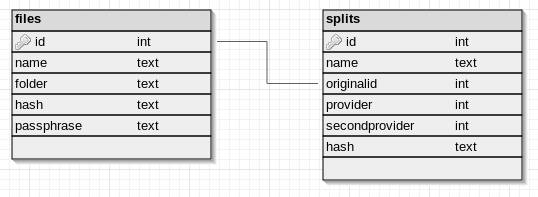
\includegraphics[scale=0.6]{resources/Bilder_Kapitel_5/sql.png}
  \caption{Schema der SQLite Datenbank}
  \label{fig-implementierung-sql}
\end{figure}

Die Tabelle \frqq files\flqq\ speichert Informationen zur Originaldatei, den Namen, den Ordner in dem diese auf dem lokalen Dateisystem gespeichert ist, sowie den Hash des Inhalts und den Passphrase zum Ent- und Verschlüsseln der Datei.
Der Hash wird benötigt um nach dem Download einer Datei und der Durchführung der Dateioperation zu prüfen, ob die Datei korrekt wiederhergestellt wurde.

In Tabelle \frqq splits\flqq\ werden die Informationen zu den Teilstücke einer Datei gespeichert.
Neben dem Namen und der Verknüpfung zur ursprünglichen Datei, hier \frqq originalid\flqq\ genannt, wird ein weiterer Hash gespeichert und die Provider, bei denen die Datei geuploaded wurde.
Der Wert \frqq providerid\flqq\ entspricht der ID aus der \ac{JSON} Datei, welche im Quellcode \ref{fig-implementierung-provider-json} aufgeführt ist.
Somit können programmatisch die Teilstücke von den einzelnen Anbietern geladen werden.
Nachdem der Download beendet ist, werden die Teilstücke mit den in der Datenbank gespeicherten Hashwerten verglichen, um auch in diesem Fall die Dateiintegrität sicherzustellen.

% ##############################################################################
% ################## Realisierung der Anwendungslogik-Schicht ##################
% ##############################################################################
\section{Realisierung der Anwendungslogik-Schicht}
\label{implementierung-realisierung-anwendungslogik}
Der Workflow der Anwendungslogik-Schicht beginnt mit dem Initialisieren der Anwendung.
Hierbei wird als Erstes die Konsistenz der benötigten Ordner überprüft.
Dazu zählen der temp, logging und models Ordner.
Sollte einer dieser drei Ordner nicht existieren, wird er von der Anwendung angelegt.
Daraufhin werden die \ac{JSON} Dateien im models Ordner überprüft.
Sollten auch diese nicht vorhanden sein, werden sie angelegt und mit Standardwerten gefüllt.
Als weiterer Schritt wird geprüft, ob die SQLite Datenbank existiert.
Sofern sich auch diese nicht im models Ordner befindet, wird sie angelegt und die beiden Tabellen erzeugt.
Abschließend wird der temp Ordner geleert, für den Fall, dass sich noch temporäre Dateien in diesem befinden.
Dieser Vorgang wird sowohl beim ersten Starten der Anwendung durchgeführt, als auch bei jedem weiteren Start.
Eine Unterscheidung dieser beiden Vorgänge wird nicht getroffen.

Wenn sich die Daten der Anwendung daraufhin in einem konsistenten Zustand befinden, werden alle Einstellungen geladen.
Die Daten aus den \ac{JSON} Dateien werden gelesen und in einer globale Variable im System hinterlegt.
Das ermöglicht bei der Ausführung von CloudGrid einen schnelleren Zugriff auf diese Daten und vermindert die Anzahl der Zugriffe auf das Dateisystem.

Sobald auch dieser Vorgang abgeschlossen ist, wird parallel der Webserver und die Ordnerüberwachung gestartet.
Auf Seiten des Webservers werden dazu alle Einstellungen geladen, wie beispielsweise der Port, auf dem die Webseite laufen soll, die Templateengine wird festgelegt und die einzelnen Standardtemplates vorgeladen.
Zusätzlich werden alle Routen definiert.
Außerdem werden die gespeicherten OAuth-Token der Cloudservices auf Aktualität geprüft.
Sollte der access token eines Services abgelaufen sein, so wird dieser, mit Hilfe des refresh tokens, erneuert.

Die Initialisierung der Ordnerüberwachung erfolgt in mehreren Schritten.
Als Erstes wird das aktuelle Dateisystem auf Veränderungen überprüft.
Dazu werden, mit der selbsterstellen Klasse \frqq foldertree\flqq , alle Dateien erfasst und deren Hashwert ermittelt, um diese daraufhin mit dem Hashwert in der Datenbank zu vergleichen.
Sollten die diese nicht übereinstimmen, so werden zuerst die Teilstücke der Datei bei den Cloudservices gelöscht, um danach die Dateioperationen auf die Datei anzuwenden und diese anschließend auf die Cloudservices zu verteilen.
Wenn jedoch eine Datei nicht in der Datenbank existiert, so wird diese in die Datenbank aufgenommen, die Dateioperationen angewendet und entsprechend zu den Cloudservices hochgeladen.
Abschließend werden gelöschte Dateien ermittelt, das bedeutet, alle Dateien welche sich in der Datenbank befinden, jedoch nicht auf dem Dateisystem.
Wenn dieser Fall eintritt, werden sowohl die Teilstücke auf den Cloudservices, als auch die Informationen über die Datei aus der Datenbank gelöscht.

Wenn dieser Vorgang beendet ist, wird die Konsistenz der Teilstücke bei den Cloudservices überprüft.
Dazu werden die Informationen zu den Teilstücken aus der Datenbank ausgelesen und selbige auf Existenz bei den Cloudservices geprüft.
Wenn ein Teilstück fehlen sollte, wird versucht dieses bei dem redundanten Cloudservices herunterzuladen und erneut hochzuladen.
Sollte das Teilstück bei allen Cloudservices gelöscht worden sein, so werden alle Teilstücke der originalen Datei auf den Cloudservices gelöscht, sowie die Informationen in der Datenbank, um die Datei daraufhin wie eine Neuanlage zu betrachten und den bereits beschriebenen Vorgang durchzuführen.

Nach der erfolgreichen Durchführung dieses Vorganges wird letztendlich die Ordnerüberwachung gestartet.
Diese überwacht einen vom Benutzer angegebenen Ordner auf Veränderung.
Dabei können die in Abschnitt \ref{systementwurf-dateihandling} beschriebenen Dateioperationen, anlegen, löschen, bearbeiten, umbenennen und verschieben einer Datei, auftreten.
Jeder dieser Fälle muss einzeln abgearbeitet werden.
Um sicherzustellen, dass die einzelnen Funktionen erfolgreich durchgeführt werden können und sich beim Zugriff auf die Datenbank nicht gegenseitig blockieren, werden sie, unter Zuhilfenahme der queue Klasse, in eine Warteschlange eingefügt.
Diese führt alle dort enthaltenden Funktionen nacheinander aus, sodass keine gleichzeitigen Zugriffe auftreten können.

\paragraph{Anlegen:}Beim anlegen einer Datei wird die Methode \frqq createProcess\flqq\ ausgeführt.
Diese prüft zuerst, ob die angegebene Datei wirklich existiert und ob es sich um eine Datei oder einen Ordner handelt.
Sollte die Datei nicht existieren oder ein Ordner übergeben worden sein, so bricht die Methode mit einer Fehlermeldung ab.
Ansonsten beginnt sie mit der Komprimierung der Datei.
Dabei wird eine Funktion aus dem filehelper verwendet.
Zum Komprimieren wird die Node.js eigene \frqq zlib\flqq\ Klasse verwendet.
Eine Datei, die komprimiert wurde, wird in dem temp Ordner der Anwendung gespeichert und mit der Dateiendung \frqq zip\flqq\ versehen.
Sollte dieser Vorgang erfolgreich gewesen sein, so wird ein Passphrase erstellt und die Datei daraufhin verschlüsselt.
Auch in diesem Fall wird die Datei im temp Ordner gespeichert und mit der Dateiendung \frqq crypt\flqq\ versehen.
Nach der erfolgreichen Verschlüsselung wird die Datei gesplittet.
Dazu wird zuerst die Anzahl der eingebundenen Cloudservices ermittelt, um anhand dieser die Anzahl der Teilstücken zu bestimmen.
Beim Splitten wird jedes Teilstück mit einem pseudozufälligen Dateinamen versehen und im temp Ordner gespeichert.
Im Anschluss daran werden die eingebundenen Cloudservices ausgewählt und der Upload der Dateien wird durchgeführt.
Abschließend werden alle Informationen zur originalen Datei und zu den Teilstücken in der SQLite Datenbank gespeichert und alle temporären Dateien aus dem temp Ordner gelöscht.
Sollte in dem gesamten Prozess ein Fehler auftreten, so wird dieser unter Zuhilfenahme der \frqq infologger\flqq\ Funktionssammlung in eine Logging Datei geschrieben und kann vom Benutzer in der \ac{GUI} eingesehen werden.
Der Prozess selbst wird abgebrochen und der nächste Prozess gestartet, insofern es einen weiteren in der Queue gibt.

\paragraph{Löschen:}Beim Löschen einer Datei wird die Methode \frqq deleteProcess\flqq\ ausgeführt.
Diese ermittelt zuerst die Datenbank ID der originalen Datei, um daraufhin alle Teilstücke zu selektieren.
Sobald diese Informationen vorliegen, werden alle Teilstücke bei allen Cloudservices gelöscht.
Dazu werden die entsprechenden Methoden in den Provider Klassen ausgeführt.
Abschließend werden die Einträge in den Datenbanken gelöscht.
Auch die deleteProcess Methode wird durch die infologger Funktionssammlung protokolliert und an die Queue übergeben.

\paragraph{Bearbeiten:}Die Bearbeitung einer Datei ähnelt einer Vereinigung der beiden zuvor vorgestellten Prozesse.
Sollte sich der Inhalt einer Datei verändern, werden zuerst alle Teilstücke einer Datei auf den Cloudservices und zugleich deren Informationen aus der Datenbank gelöscht.
Die Informationen zu der originalen Datei bleiben in der Tabelle files in der Datenbank erhalten.
Daraufhin wird der Hash der Datei neu berechnet und der Datenbankeintrag entsprechend geupdatet.
Anschließend werden die Dateioperationen, welche auch im \frqq createProcess\flqq\ durchgeführt wurden, ausgeführt.
Die Teilstücke werden dann zu den Cloudservices hochgeladen und die Informationen in die Datenbank geschrieben.

\paragraph{Umbenennen/Verschieben:}Zum Zeitpunkt der Erstellung der Arbeit bietet das Modul \frqq watchr\flqq\ keine Methoden zum Erkennen einer Umbenennung oder Verschiebung einer Datei.
Dadurch ergibt sich ein großer Nachteil bei der Implementierung in CloudGrid.
Normalerweise würde lediglich der Dateiname beziehungsweise der Pfad zur Datei in der Datenbank angepasst werden und die Teilstücke einer Datei bei den Cloudservices könnten unverändert bleiben.
Durch das Fehlen der Methode wird das Umbenennen und auch das Verschieben einer Datei als Löschen und anschließend Erstellen einer Datei angesehen.
Das beeinträchtigt erheblich die Effizienz von CloudGrid.
Dieser Umstand muss in einer späteren Version des Prototypen angepasst werden, um unnötige Datei- und Uploadoperationen zu vermeiden und die Effizienz bei der Ausführung der Anwendung zu steigern.

Die Ordnerüberwachung läuft solange eine Internetverbindung besteht.
Vor der Überwachung wird eine Funktion gestartet, welche im Sekundentakt prüft, ob eine Verbindung zum Internet besteht oder nicht.
Sollte diese unterbrochen werden, so wird auch die Ordnerüberwachung gestoppt und die Queue mit den Prozessen geleert.
Dieser Vorgang wird durch die Funktion \frqq hasInternet\flqq\ der \frqq utils\flqq\ Funktionssammlung realisiert.
Um die Überprüfung umzusetzen, wird ein Datenpaket mittels Ping an google.de geschickt.
Sollte ein Datenpaket zurückgeschickt werden, besteht eine Internetverbindung, ansonsten nicht.
Wenn die Verbindung zum Internet wieder aufgebaut wurde, wird automatisch die Ordnerüberwachung gestartet und der zuvor aufgezeigte Vorgang erneut durchgeführt.
Dadurch, dass die initiale Überprüfung der Dateien durchgeführt wird, werden auch Prozesse, die zuvor aus der Queue gelöscht wurden, erneut ausgeführt.

% ###########################################################################
% ################## Realisierung der Präsentationsschicht ##################
% ###########################################################################
\section{Realisierung der Präsentationsschicht}
Die Umsetzung der Präsentationsschicht ist bewusst einfach gehalten.
Zur Gestaltung wurde \ac{CSS} verwendet, welches aus \ac{Sass} Dateien generiert wird.
\ac{Sass} ist eine Scriptsprache, welche eine programmatische Erstellung von \ac{CSS} Dateien ermöglicht.
Insbesondere die Verwendung von Variablen und Funktionen, Mixins genannt, erleichtern die Arbeit mit \ac{CSS} erheblich, wodurch das Stylesheet sich später flexibler anpassen lässt.
Eine \ac{Sass} Datei muss nach der Erstellung kompiliert werden, was der mitgelieferte \ac{Sass}-Compiler realisiert.

Bei der Umsetzung des Designs für die \ac{GUI} werden vier \ac{CSS} Dateien verwendet.
Die \frqq normalize.scss\flqq\ dient dazu, die Voreinstellungen von \ac{HTML} Elementen in verschiedenen Browsern zurückzusetzen.
Hierbei wird das normalize Projekt\footnote{\url{https://github.com/necolas/normalize.css}} verwendet.
Diese steht unter der MIT Lizenz und kann somit frei verwendet werden.

Die zweite Datei \frqq mixins.scss\flqq\ ist eine selbsterstellte Funktionssammlung, welche sich wiederholende Style-Definitionen umsetzt.
Beispielsweise dient das Mixin \frqq clearfix\flqq\ dazu, gefloatete Elemente zu clearen oder das \frqq center-page\flqq\ Mixin, um den Header, Footer und Contentbereich in der Seite zu zentrieren.

Die \frqq variables.scss\flqq\ Datei beinhaltet alle Variablen, welche in den \ac{Sass} Dateien verwendet werden.
Der Vorteil hierbei ist, dass das Farbkonzept der Seite schnell bearbeitet werden kann, da alle Farben in entsprechende Variablen ausgelagert wurden.
So können Themes angelegt werden, ohne das eine komplette \ac{CSS} oder \ac{Sass} Datei refactored werden muss.

Abschließend existiert noch die \frqq main.scss\flqq\ .
Diese beinhaltet alle Styleangaben für die einzelnen Elemente der Webseite.
Jede der zuvor genannten Dateien wird am Anfang der \frqq main.scss\flqq\ eingebunden, sodass beispielsweise auf alle Variablen oder Mixins zugegriffen werden kann.

Die Umsetzung des Grundgerüsts der Webseite erfolgt nach dem im Abschnitt \ref{systementwurf-praesentation} erstellten Wireframe.
Alle dort angedachten Konzepte wurden umgesetzt.
Wohingegen das Farbkonzept minimalistisch gehalten wurde, was bedeutet, dass lediglich Weiß, ein heller Grauton und ein dunkler Grauton verwendet werden.
Als akzentuierende Farbe für Buttons und Links wird hingegen ein Blauton verwendet.
Das Logo von CloudGrid, welches in Abbildung \ref{fig-demo-logo} aufgezeigt wird, wurde selbst entwickelt und soll ein stark abstrahiertes Grid-Cluster aufzeigen, wobei die einzelnen Nodes entsprechend farblich getrennt werden.
Somit soll die Dateiverteilung, welche in CloudGrid erfolgt, aufgezeigt und zugleich die Speicherung bei den unterschiedlichen Cloudservices erkenntlich gemacht werden.

\begin{figure}[H]
  \centering
  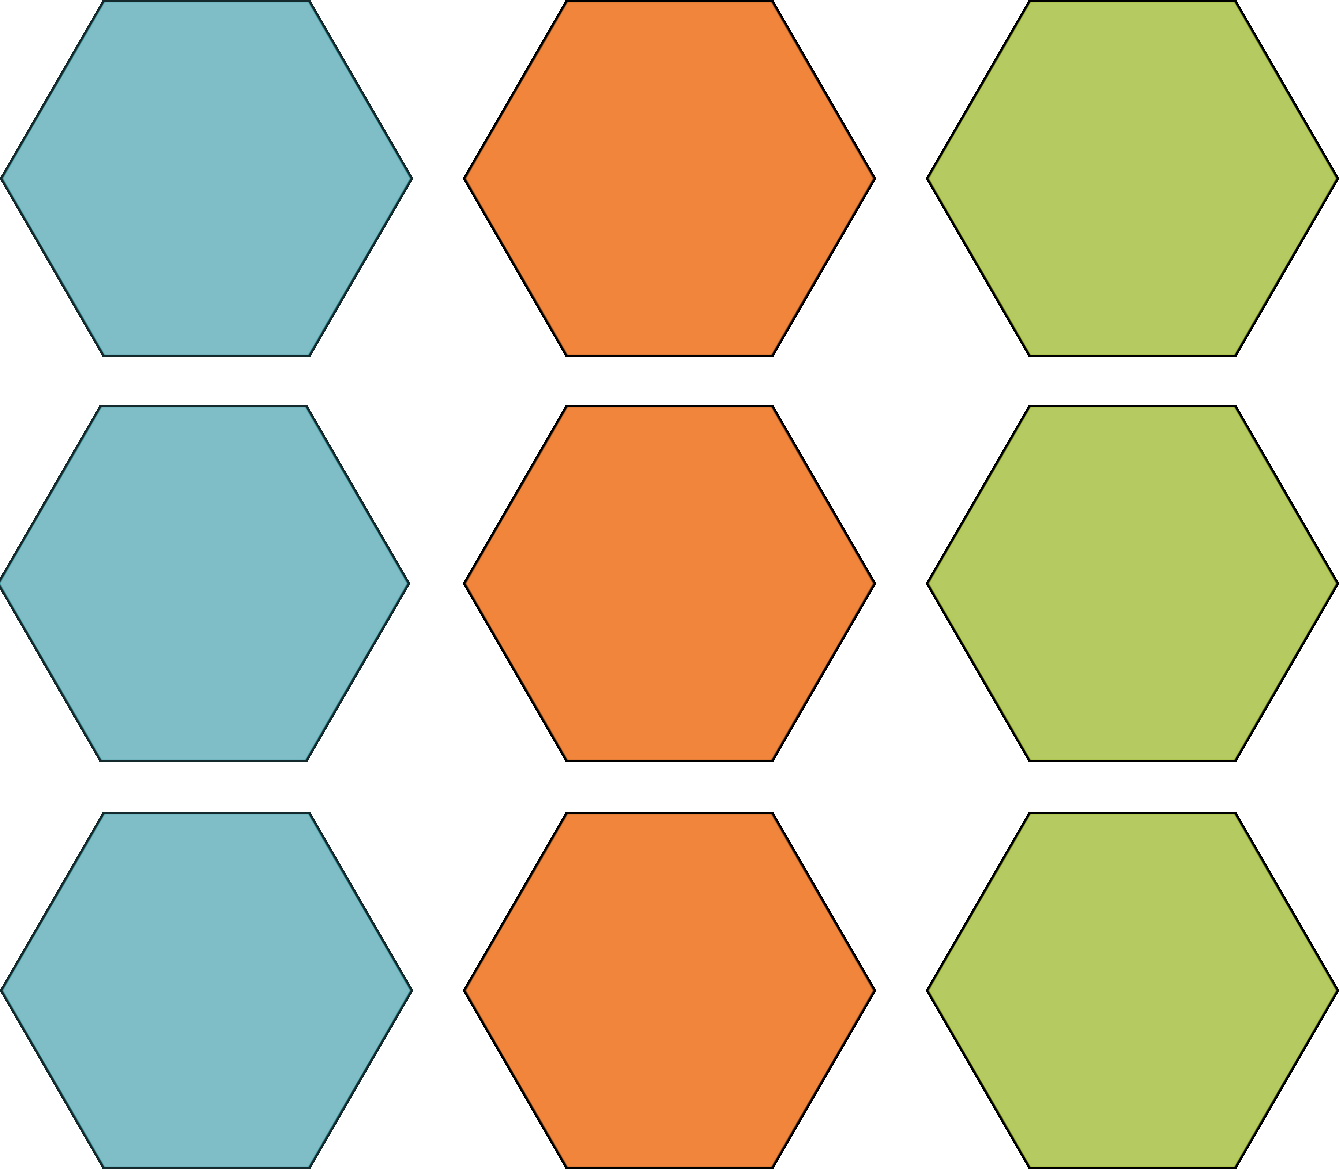
\includegraphics[scale=0.04]{resources/Bilder_Kapitel_5/logo.png}
  \caption{Das Logo von CloudGrid}
  \label{fig-demo-logo}
\end{figure}

Templates wurden, wie bereits in Abschnitt \ref{systementwurf-praesentation} beschreiben, mit der Hogan.js Templateengine umgesetzt.
Dazu werden generelle Bausteine in dem Unterordner \frqq templates\flqq\ gespeichert.
Hier existieren zwei Bausteine, einer für den Header der Seite, demnach der komplette Bereich bis zum Content und der Footer, welches nach dem Contentbereich beginnt.
Im Header werden alle benötigten \ac{CSS} Dateien eingebunden, sowie das Menü der Seite.
Wohingegen im Footer alle JavaScript Dateien eingebunden werden.
Das hat den Vorteil, dass die Ladezeit der Seite minimiert wird, da die verminderte Anzahl von \ac{HTTP} Request vor der Darstellung der Seite vermindert werden.

Neben dem Design wurde auch der Aufbau der einzelnen Seiten schlicht gehalten, damit der Benutzer sich leicht in die \ac{GUI} von CloudGrid einarbeiten kann.
Die Seite \frqq Informationen\flqq\ verfügt neben der obligatorischen Überschrift und dem Hilfe-Icon nur über eine Textbox.
Diese gibt den Inhalt der Loggingdatei des aktuellen Tages aus.
Weiterhin erhält der Benutzer die Möglichkeit das Datum der anzuzeigenden Datei durch einen entsprechenden Button zu verändern.

In der Seite \frqq Einstellungen\flqq\ kann der Benutzer jegliche personenbezogenen Einstellungen verändern.
Dazu zählen beispielsweise der Port, auf dem der Webserver läuft, und die ausgewählte Sprache.
Beim ersten Start der Anwendung wird eine ähnliche Seite angezeigt, auf der jedoch mehr Einstellungen anpassbar sind.
Beispielsweise kann der Ordner bestimmt werden, welcher von CloudGrid überwacht werden soll.
Zudem bieten beide Seiten die Möglichkeit, die Authentifizierung für die Cloudservices durchzuführen.
Dazu muss lediglich der entsprechende Button des Anbieters angeklickt werden und der in Abschnitt \ref{authentifizierung-oauth-2} aufgezeigte Authentifizierungsprozess wird gestartet.
Sobald der Benutzer vom Anbieter zurückgeleitet wird, bekommt er eine Informationen über die erfolgreiche Implementierung des Anbieters angezeigt.
Zusätzlich wird diese Information in die Logging-Datei geschrieben.


% Chapter 5
\chapter{Evaluation und Demonstration}
In diesem Kapitel sollen die Ergebnisse des im Rahmen der Arbeit entwickelten Prototypen, anhand der zuvor definierten Anforderungen und Lösungen, bewertet und vorgestellt werden.
Im Anschluss daran wird eine Demonstration des Systems durchgeführt.

\section{Evaluation des Systems}
\label{evaluation-des-system}
Der Prototyp von CloudGrid wurde ausschließlich auf einem Linux Mint System getestet und ist dort voll lauffähig.
Linux Mint basiert auf Ubuntu, sodass die zwei meistgenutzten Linux Distributionen\footnote{\url{http://distrowatch.com/dwres.php?resource=popularity}} unterstützt werden.
Sowohl Windows als auch Mac OS wurden bei der Entwicklung des Prototypen nicht getestet.

Um die GUI korrekt darstellen zu können, werden Browser benötigt, welche HTML5 und CSS3 unterstützen.
Dazu zählen Google Chrome, Firefox, Safari und auch Opera, sowie die Internet Explorer ab Version 10.
Es kann bei unterschiedlichen Browsern kleinere Abweichungen bei der Positionierung von Elementen geben, welche sich jedoch nicht auf die Funktionalität der GUI auswirken.
Dieses Verhalten resultiert aus der unterschiedlichen Interpretation von \ac{HTML} und \ac{CSS} der einzelnen Browser.

Ein weiterer Schwerpunkt liegt in der Integration weiterer Cloudservices in CloudGrid.
Wenn ein Dienst zur Anwendung hinzugefügt werden soll, müssen dazu drei Anpassungen vorgenommen werden.
In den Ordner \frqq provider\flqq\ muss zuerst eine Klasse integriert werden, welche, entsprechend der Klassen der bestehenden Anbieter, die Funktionalitäten der Clouddienste abbildet.
Daraufhin muss der einzubindende Anbieter in der Konfigurationsdatei \frqq provider.json\flqq\ im Ordner \frqq models\flqq\ aufgenommen werden.
In dieser Datei werden alle Parameter, die bei der Authentifizierung mittels OAuth benötigt werden, hinterlegt.
Um abschließend den Anbieter auch in der \ac{GUI} verfügbar zu machen, muss ein Button in der View \frqq connect.html\flqq\ hinterlegt werden, so wie die entsprechende Controllerlogik in der \frqq connect.js\flqq .
Die Auswahl der Cloudservices beim Upload wird daraufhin automatisch von CloudGrid durchgeführt.
Der gesamte Vorgang sollte, in einer späteren Version von CloudGrid, noch modularer und generischer gestaltet werden, sodass ein Entwickler leichter weitere Anbieter integrieren kann.

Weiterhin erweist sich die im Systementwurf getätigte Annahme, dass der Dateiupload, weitaus langsamer ist, als die Dateioperationen als richtig.
Bei einem Test mit einer 50 \ac{MB} großen Datei und lediglich einem Cloudservice, dauerten die Dateioperationen im Durchschnitt 7 Sekunden, wohingegen der Upload der Teilstücke im Durchschnitt rund 2 Minuten dauerte.
Diese Werte wurden auf einem Laptop mit einem Intel Core i3 mit 2,4 \ac{GHz}, 3 \ac{GB} Arbeitsspeicher, sowie einer Festplatte mit einem \ac{SATA} Anschluss und 7200 \ac{upm} ermittelt.
Die Uploadgeschwindigkeit wird laut Internetprovider mit 10 mbit/s angegeben.
Dieser Engpass kann leider nicht umgangen werden.
Vor dem Upload der Teilstücke einer Datei, werden diese bereits komprimiert, um den Vorgang zu beschleunigen.
Jedoch reicht das nicht aus, um das Verhältnis auszugleichen.
Dateioperationen werden zum jetzigen Stand der Technik schneller durchgeführt, als das Verschicken von Daten über ein Netzwerk oder das Internet.
Lediglich durch die Implementierung der, bereits im Abschnitt \ref{implementierung-realisierung-anwendungslogik} erwähnten fehlenden Unterstützung der Events \frqq Verschieben\flqq\ und \frqq Umbenennen\flqq\ bei der Ordnerüberwachung, können unnötige Uploadvorgänge vermieden werden, was Ressourcen einsparen würde.
Jedoch bleibt auch dadurch die Grundproblematik bestehen.

\section{Demonstration des Systems}

Um die Anwendung zu starten muss die Linux Konsole geöffnet werden und in den entsprechenden Ordner von CloudGrid navigiert werden.
Dort muss entweder der Befehl \frqq node CloudGrid.js\flqq\ oder alternativ die Makefile mittels \frqq make start\flqq\ ausgeführt werden.
Daraufhin ist die \ac{GUI} im Browser unter \url{http://localhost:8080} oder alternativ unter \url{http://cloudgrid.local:8080} erreichbar.
Beim ersten Start der Anwendung bekommt der Benutzer eine Einstellungsseite angezeigt, welche in Abbildung \ref{fig-demo-first-start} zu sehen ist.

\begin{figure}[H]
  \centering
  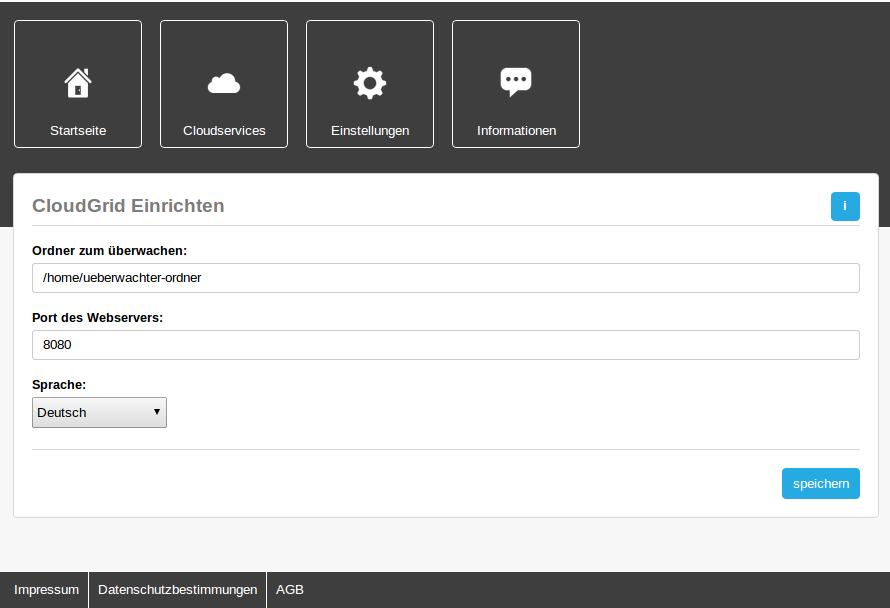
\includegraphics[scale=0.4]{resources/Bilder_Kapitel_6/first-start.png}
  \caption{Einstellungsseite beim ersten Start der Anwendung}
  \label{fig-demo-first-start}
\end{figure}

Hier kann der Benutzer den zu überwachenden Ordner, den Port auf dem der Webserver laufen soll und die Sprache einstellen.
Dabei sind alle Werte vordefiniert, sodass der Nutzer sich leichter in diese Seite einfinden kann.
Durch Anklicken des blauen \frqq i\flqq\ Buttons in der rechten oberen Ecke erhält er darüber hinaus Informationen zur Seite.
Wenn er die Einstellungen gespeichert hat, wird eine Erfolgsseite angezeigt.
Sollte er Felder nicht ausfüllen, erscheint eine entsprechend Fehlermeldung und die Felder können nochmals bearbeitet werden.

Sobald die Speicherung erfolgreich war, muss sich der Benutzer im Menüpunkt \frqq Cloudservices\flqq\ mit den einzelnen Diensten verbinden.
Abbildung \ref{fig-demo-cloudservices} zeigt diese Seite auf.
Der Benutzer muss zuvor seine \frqq client id\frqq , seinen \frqq client secret\flqq\ und die \frqq redirect uri\flqq\ in den entsprechenden Formularfelder hinterlegen, um daraufhin durch einen Klick auf das entsprechende Logo des Anbieters, die Authentifizierung durchzuführen.
Er wird daraufhin zum Anbieter weitergeleitet, wo er sich Einloggen muss, um dann CloudGrid die Berechtigung zu geben, auf seine Benutzerdaten zuzugreifen.
Abschließend wird er wieder zur Cloudservicesseite zurückgeleitet und erhält einen Hinweis, über die erfolgreiche Verknüpfung mit dem Service.
Dienste welche bereits erfolgreich verbunden sind, erhalten einen grünen Haken am Logo, nicht verbundene Dienste ein rotes Kreuz.

\begin{figure}[H]
  \centering
  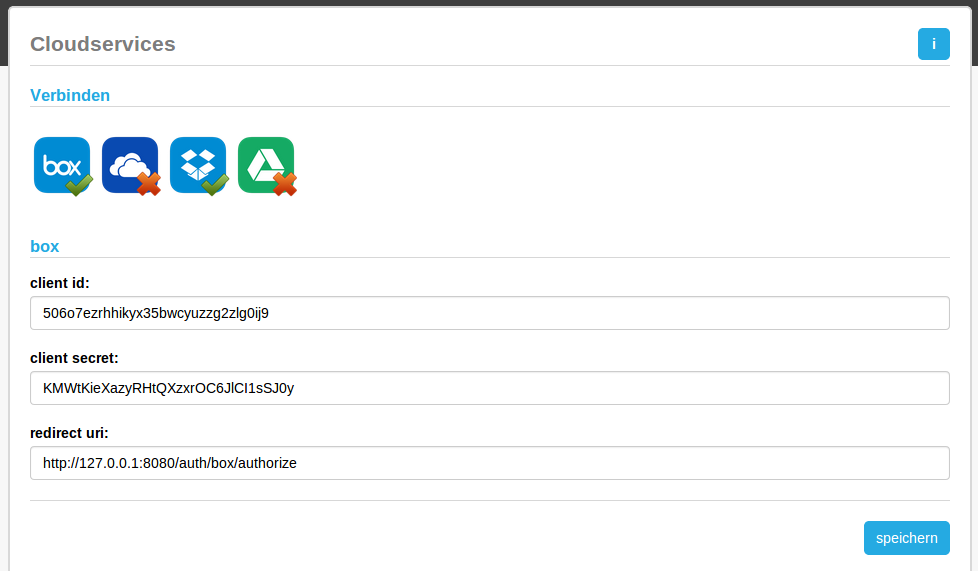
\includegraphics[scale=0.4]{resources/Bilder_Kapitel_6/cloudservices.png}
  \caption{Seite zum Verbinden und Bearbeiten der Cloudservices}
  \label{fig-demo-cloudservices}
\end{figure}

Wenn auch dieser Vorgang abgeschlossen ist, kann der Benutzer Ordnerüberwachung zum ersten mal starten.
Im Header der \ac{GUI} befindet sich ein Button, welcher betätigt werden muss.
Initial ist die Ordnerüberwachung deaktiviert.
Abbildung \ref{fig-demo-watchr-not-started} zeigt den Informationstext und den Button auf.

\begin{figure}[H]
  \centering
  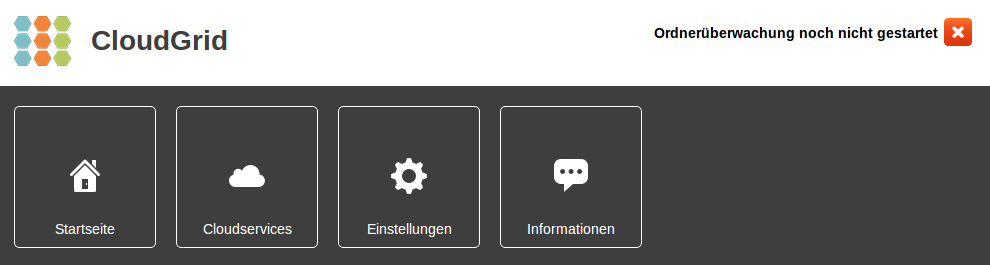
\includegraphics[scale=0.4]{resources/Bilder_Kapitel_6/watchr_not_started.png}
  \caption{Die Ordnerüberwachung ist deaktiviert}
  \label{fig-demo-watchr-not-started}
\end{figure}

Sobald der Benutzer den Button anklickt, wird eine Warteanimation gestartet.
Wenn der Vorgang abgeschlossen ist, bekommt er die Information, welche in Abbildung \ref{fig-demo-watchr-started} dargestellt ist, angezeigt.

\begin{figure}[H]
  \centering
  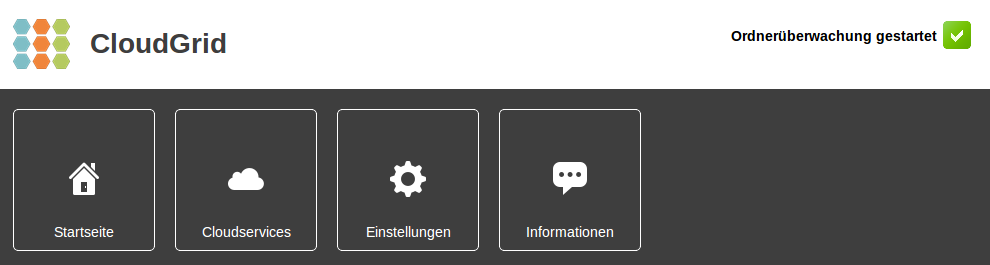
\includegraphics[scale=0.4]{resources/Bilder_Kapitel_6/watchr_started.png}
  \caption{Die Ordnerüberwachung wurde gestartet}
  \label{fig-demo-watchr-started}
\end{figure}

Die Ordnerüberwachung ist somit gestartet und jegliche Veränderungen werden erkannt.
Alle Dateien, welche sich in dem zu überwachenden Ordner befinden, werden zudem beim Start initial eingelesen und zu den Clouddiensten geuploaded.
Der Benutzer hat jederzeit die Möglichkeit, die Ordnerüberwachung an- und abzustellen.
Dieses Verhalten kann gewünscht sein, wenn beispielsweise größere Veränderungen in dem Ordner durchgeführt werden oder die gesamte Bandbreite der Internetverbindung benötigt wird.

Jegliche Vorgänge kann der Benutzer dabei im Menüpunkt \frqq Informationen\flqq\ einsehen und den Fortschritt verfolgen.
Abbildung \ref{fig-demo-logging} zeigt beispielhaft diese Seite auf.
Die Einträge in dem Textfeld werden im zwei Sekundentakt aktualisiert, sodass der Benutzer die Seite nicht manuell aktualisieren muss.
Zudem kann er sich ältere Einträge mittels der Datumsauswahl oberhalb des Informationsfensters anzeigen lassen.

\begin{figure}[H]
  \centering
  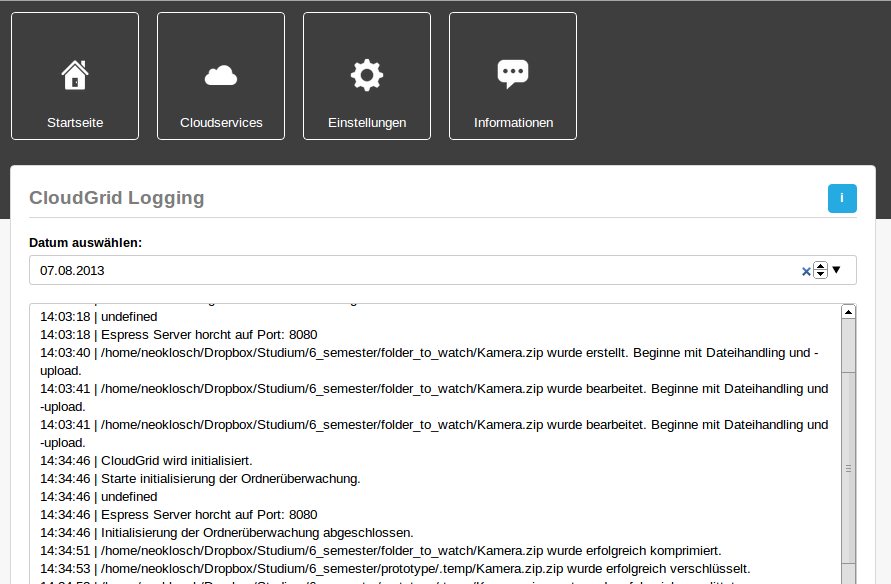
\includegraphics[scale=0.4]{resources/Bilder_Kapitel_6/logging.png}
  \caption{Informationsseite von CloudGrid}
  \label{fig-demo-logging}
\end{figure}

Die Seite \frqq Einstellungen\flqq\ ähnelt der Seite, die der Benutzer beim ersten Start der Anwendung angezeigt bekommt.
Jedoch sind hier weniger Einstellmöglichkeiten verfügbar.
Im Prototypen ist es nicht möglich, den zu überprüfenden Ordner zu wechseln.
Das Problem liegt in einer erhöhten Komplexität des Dateihandlings.
Es muss geklärt werden, was mit den Dateien im bestehenden Ordner passiert.
Dabei können zwei Ansätze verfolgt werden.
Im ersten Fall werden alle Dateien in den neu zu überwachenden Ordner kopiert und verbleiben bei den Clouddiensten.
Der zweite Fall belässt alle Dateien im ursprünglichen Ordner und löscht die entsprechenden Teilstücke bei den Clouddiensten.
Beide Verfahren haben ihre Vor- und Nachteile.
Im Prototypen wurde daher lediglich das einmalige Auswählen des Ordner integriert.
Jedoch können wie bereits zuvor, sowohl die Sprache, als auch der Port des Webservers bearbeitet werden.

Im Footer der Seite wurden hingegen die drei Seiten \frqq Impressum\flqq , \frqq AGB\flqq\ und \frqq Datenschutz\flqq\ aufgenommen.
Da diese funktional nicht relevant sind, sind sie momentan mit Blindtext gefüllt, bedingt durch die im Abschnitt \ref{systementwurf-recht} erwähnte Problematik, dass diese inhaltlich durch einen Anwalt erstellt werden müssen.

Letztendlich wurde das in Abschnitt \ref{systementwurf-praesentation} angedachte Designkonzept komplett umgesetzt und erfüllt funktional alle Anforderungen.
Auf allen Seiten ist ein einheitliches Layout zu erkennen, welches mit der \frqq hogan\flqq\ Templateengine modular umgesetzt wurde.


% Chapter 6
\chapter{Zusammenfassung und Ausblick}
Ziel dieser Arbeit war es, einen Prototypen zu entwickeln, der die Möglichkeiten des Dateimanagements unter Verwendung verschiedener Cloudservices aufzeigt.

Um die gestellte Aufgabe zu lösen, wurden in der Anforderungsanalyse die Voraussetzungen für das System dargelegt.
Dabei wurde das grobe Konzept des Prototypen erklärt und die unterschiedlichen Anforderungen an die Cloudservices und die zu verwendenden Technologien erarbeitet.
Weiterhin dienten die erstellten Use-Cases dem besseren Verständnis der Funktionsweise des Prototypen.
Die Evaluation bestehender Anwendung und Dienste zeigt Umsetzungsmöglichkeiten und zugleich Abgrenzungskriterien für CloudGrid auf.

Anschließend wurde im Kapitel Systementwurf konkreter auf die geplante Umsetzung des Prototypen eingegangen.
Dabei wurde sowohl die zu verwendende Programmierumgebung ermittelt, als auch die Architektur des Systems aufgezeigt.
Diese konnte in drei Schichten, Datenhaltungs-, Anwendungslogik- und Präsentationsschicht, unterteilt werden.
Die Evaluation der Cloudservices wertete, sowohl aus technischer, als auch aus rechtlicher Sicht, bestehende Dienste, anhand der zuvor definierten Kriterien, aus.

Die konkrete Umsetzung des Prototypen wurde daraufhin im Kapitel Implementierung ausgearbeitet.
Dazu wurde neben der Projektstruktur, die Funktionsweise externer und auch selbst entwickelter Module erklärt und deren Einbindung in das System erläutert.
Weiterhin wurden die Realisierung der einzelnen Schichten erörtert.

Abschließend wurde im Abschnitt Evaluation und Demonstration der entwickelte Prototyp bewertet und die Handhabung, sowie die Funktionsweise, aufgezeigt.

Im Prototypen von CloudGrid wurden alle zuvor erarbeiteten Anforderungen umgesetzt.
Bei einer zukünftige Weiterentwicklung des vorgestellten Systems sollte primär auf eine Erweiterung des Cloudservice Portfolios gesetzt werden.
Um dies zu realisieren, sollten sowohl mehr Authentifizierungsmethoden unterstützt werden, als auch das Datenformat \ac{XML}, da dies von mehreren Anbietern verwendet wird.
Dadurch könnten bereits vier weitere, der in Abschnitt \ref{systementwurf-cloudanbieter} evaluierten Anbieter, eingebunden werden.
Darüber hinaus würde die Anzahl nochmals steigen, wenn auch kostenpflichtige Anbieter hinzugefügt werden.
Jedoch bleibt der Nachteil bestehen, dass anbieterspezifische Funktion nicht in CloudGrid integrierbar sind, wie beispielsweise die Versionierung von Dropbox.

Weiterhin sollte eine Synchronisierung über mehrere Clients realisiert werden.
Das erhöht die Nutzbarkeit für den Anwender und entspricht der Funktionalität aktueller Clientanwendungen der Anbieter.
Hierbei müssen wahrscheinlich größere systemarchitektonische Anpassungen vorgenommen werden.
Ein Konzept wäre, die lokalen Benutzerdaten von CloudGrid ebenfalls redundant bei den Cloudservices vorzuhalten, um diese auf einem weiteren Client einzubinden.
Ebenfalls denkbar wäre die Einbindung eines weiteren Serverdienstes, der die entsprechenden Informationen vorhält.
Allerdings ist diese Möglichkeit abweichend von der momentanen Grundidee von CloudGrid, dem Benutzer ein System zu ermöglichen, bei dem er jederzeit Überblick über den Verbleib seiner Daten hat.

Zudem würde die Umsetzung mobiler Anwendungen, für Smartphones und Tablets, die Anwenderfreundlichkeit erhöhen.
Auch hier müssten konzeptionelle Änderungen durchgeführt werden, welche sich möglicherweise mit denen des Multiclient Konzepts gleichen.

Auf Seiten der Node.js Anwendung würde die Erweiterung des \frqq watchr\flqq\ Moduls um die Events \frqq Umbenennen\flqq\ und \frqq Verschieben\flqq\ die Performance steigern und unnötige Dateioperationen vermeiden.
Weiterhin ist es möglich, weitere Einstellungsmöglichkeiten, wie das Setzen eines anderen oder eines weiteren zu überprüfenden Ordners oder auch die Wahl des Verschlüsselungsalgorithmus.
Dabei muss jedoch beachtet werden, dass sich solch eine Option auf bereits hochgeladene Dateien auswirken würde.

Wie bereits in Abschnitt \ref{evaluation-des-system} beschrieben, sollte auch die Einbindung weiterer Cloudservices modularer und generischer gestaltet werden.
Momentan müssen mehrere Dateien bearbeitet werden, um einen Dienst zu CloudGrid hinzuzufügen.
Besser wäre es, wenn es einen Ordner geben würde, wo Module für Cloudservices vorgehalten und weitere hinzugefügt werden können.
Dieser wird beim Systemstart auf neue Module geprüft und diese entsprechend eingebunden.

Abschließend sollte die \ac{GUI} erweitert werden, um die Benutzerfreundlichkeit zu steigern.
Dazu zählen mehr Informationen für den Benutzer, wie beispielsweise ein Hinweis, wenn der Speicherplatz eines Anbieters ausgereizt ist oder ein Anbieter nicht mehr verfügbar ist.

Letztendlich zeigt das hier vorgestellte System, erfolgreich und in einer prototypischen Qualität, die Funktionsweise des erarbeiteten Konzeptes auf.
Das Ergebnis kann somit als solide Grundlage für eine Weiterentwicklung angesehen werden.

\pagenumbering{Roman}
\setcounter{page}{1}

%\include{StandDerTechnik}
%\include{Grundlagen}
%\include{Umsetzung}
%\include{Systemarchitektur}
%
%
%
%
%\protect \addtocontents{toc}{\protect\newpage}  % Seitenumbruch im Inhaltsverzeichnis
%\cleardoublepage
%\include{ExperimentelleValidierung}
%\include{Schlussbetrachtungen}
%
%
%
%\begin{appendix}
%\include{Anhang_Mathematik}                 % A
%\include{Anhang_FormatDerParameterdateien}  % B
%\include{Anhang_Quelltexte}                 % C
%\include{Anhang_Datenblaetter}              % D
%\include{Anhang_Glossar}                    % E
%\end{appendix}
%
%
%
%% Erstes Literaturverzeichnis, ohne BibTeX
%
%\interlinepenalty=10000 % Literatureinträge: Absätze zusammenhalten
%\cleardoublepage
%\addcontentsline{toc}{chapter}{Literaturverzeichnis}
%%F�r das nachfolgende exemplarische Literaturverzeichnis wurde die einfache thebibliography-Umgebung von Latex verwendet. F�r Studien- und Diplomarbeiten mit weniger als 40 Quellen sollte diese auf jeden Fall ausreichen und hat gegen�ber dem komplexen Bibtex-Paket weiterhin den Vorteil flexiblerer Formatierungsm�glichkeiten.
%
%Im Anschluss an das exemplarische Literaturverzeichnis ist ein zweites Verzeichnis beigef�gt, welches weiterf�hrende Quellen zum vorliegenden Latex-Template enth�lt: Download-Links zur Software, freie Online-Latex-Handb�cher usw.



\begin{thebibliography}{Ti}



\bibitem[Abdel-Aziz 71]{abdelaziz71} Y. I. Abdel-Aziz and H. M. Karara, \glqq Direct linear transformation from comparator coordinates into object space coordinates in close-range photogrammetry\grqq, in: Symposium on Close-Range Photogrammetry, issue 11, pp. 1--18, University of Illinois at Urbana-Champaign, 1971.

\bibitem[AutTech 07]{auttech07} Firma Automation Technology GmbH in 22946 Trittau, Produkt�bersicht, Downloads und Datenbl�tter.  URL: \url{http://www.automationtechnology.de}

\bibitem[Dang 06]{dang06} T. Dang, C. Stiller and C. Hoffmann, \glqq Self-calibration for Active Automotive
Stereo Vision\grqq, Proc. of the IEEE Intelligent Vehicles Symposium, pp. 364--369, Japan, Tokyo, 2006.

\bibitem[Fisher 96]{fisher96} R. B. Fisher and D. K. Naidu. \glqq A Comparison of Algorithms for Subpixel Peak Detection\grqq\, in: Advances in Image Processing, Multimedia and Machine Vision, Springer-Verlag, Heidelberg, 1996. Online erh�ltlich via CiteSeer.

\bibitem[Gamma 04]{gamma04} E. Gamma, D. Riehle u.\,a., \glqq Entwurfsmuster -- Elemente wiederverwendbarer objektorientierter Software\grqq, Addison-Wesley-Verlag, M�nchen, 2004.

\bibitem[G�hring 02]{guehring02} J. G�hring, \glqq 3D-Erfassung und Objektrekonstruktion mittels Streifenprojektion\grqq, Dissertation, Universit�t Stuttgart, Institut f�r Photogrammetrie, 2002. Online erh�ltlich via URL: \url{http://elib.uni-stuttgart.de/opus/volltexte/2006/2715/pdf/Guehring_diss.pdf}

\bibitem[Hoppe 02]{hoppe02} H. Hoppe, C. K�bler, J. Raczkowsky und H. W�rn, \glqq Ein neues und leicht zu implementierendes
Modell zur pr�zisen Kalibration von Kameras und Videoprojektoren\grqq, in: Medicine Meets Virtual Reality (MMVR 02), pp. 229--232, Newport Beach, USA, 2002.

\bibitem[Huckle 02]{huckle02} T. Huckle und S. Schneider, \glqq Numerik f�r Informatiker\grqq, Springer-Verlag, Heidelberg, 2002.

\bibitem[K�ferstein 98]{kaeferstein98} B. K�ferstein, \glqq 3D-Verformungsmessungen auf 10nm genau -- Grundlagen und Anwendungen der Speckle-Interferometrie\grqq, Institutsmittelung Nr. 23, Institut f�r Maschinenwesen (IMW), Technische Universit�t Clausthal, 1998.

\bibitem[Kitware 07]{kitware07} Firma Kitware Inc. (USA), Online-Produktpr�sentation und freier Download der Software-Bibliothek VTK -- Visualization Toolkit. URL: \url{http://www.kitware.com}

\bibitem[Luhmann 03]{luhmann03} T. Luhmann, \glqq Nahbereichsphotogrammetrie: Grundlagen -- Methoden -- Anwendungen\grqq, Wichmann-Verlag, Heidelberg, 2003.

\bibitem [Marqu 63]{marqu63} D. Marquardt, \glqq An Algorithm for Least-Squares Estimation of Nonlinear Parameters\grqq, SIAM J. Appl. Math., vol. 11, pp. 431--441, 1963.

\bibitem[Pentax 07]{pentax07} Firma Pentax, Online-Produktspektrum und Datenbl�tter. URL: \url{http://www.pentax.de}

\bibitem[Pollefeys 03]{pollefeys03} M. Pollefeys, L. Van Gool u.a., \glqq3D Capture of Archaeology and Architecture with a Hand-Held Camera\grqq, Proc. of the ISPRS workshop on Vision Techniques for Digital Architectural and Archaeological Archives, Ancona, Italy, The Int. Archive of the Photogrammetry, Remote Sensing and Spatial Information Sciences, Vol. XXXIV, Part 5/W12, pp. 262--267, July 2003.

\bibitem[SAC 07]{sac07} Firma SAC GmbH in 76149 Karlsruhe, Online-Produktspektrum und Datenbl�tter. URL: \url{http://www.sac-vision.de}.

\bibitem[SuK 07]{suk07} Firma Sch�fter und Kirchhoff GmbH in 22525 Hamburg,
Online-Produktspektrum, bes. interessant: die Applikationsschriften. URL:
\url{http://www.sukhamburg.de}

\bibitem[TI 07]{ti07} Firma Texas Instruments, Online-Produktspektrum, Datenbl�tter und Downloads. URL: \url{http://www.ti.com}

\bibitem[TIS 07]{tis07} Firma The\,Imaging\,Source Europe GmbH in 28215 Bremen, Produkt�bersicht, Downloads und Datenbl�tter. URL: \url{http://www.theimagingsource.com}


\bibitem[Trolltech 07]{trolltech07} Fa. Trolltech Inc., Produktinformationen und Download zur Software-Bibliothek Qt. URL: \url{http://www.trolltech.com}

\bibitem[Trucco 98]{trucco98} E. Trucco and A. Verri, \glqq Introductory Techniques for 3-D Computer Vision\grqq, Verlag Prentice\,Hall, 1998.

\bibitem[VC 07]{vc07} Firma Vision Components in 76275 Ettlingen, Online-Produkt�bersicht, Datenbl�tter und Tutorials , URL: \url{http://www.vision-components.com}

\bibitem[Vuylsteke 90]{vuylsteke90} P. Vuylsteke and A. Oosterlinck, \glqq Range image acquisition with a single binary-encoded light pattern\grqq, Tagungsband: IEEE Transactions on Pattern Analysis and Machine Intelligence (PAMI), Vol.\,12, No.\,2, pp.\,148--164, 1990.

\bibitem[W�rn 05]{woern05} H. W�rn und U. Brinkschulte, \glqq Echtzeitsysteme\grqq, Springer-Verlag, Heidelberg, 2005.

\bibitem[Zhang 00]{zhang00} Z. Zhang, \glqq Flexible camera calibration by viewing a plane from unknown orientations\grqq, IEEE Transactions on Pattern Analysis and Machine Intelligence (PAMI), Vol.\,22, No.\,11, pp.\,1330--1334, 2000, URL: <ftp://ftp.research.microsoft.com/pub/tr/tr-98-71.pdf> (31.05.2007).

\end{thebibliography}



%
%
%
%% Zweites Literaturverzeichnis, mit BibTeX

%\begin{appendix}
%\chapter{Glossar}\index{Glossar}
\label{xx_glossar}

\interlinepenalty=10000 % keine Schusterjungen, keine Hurenkinder



\begin{description}

\item[\bf{Algorithmus}] a

\item[\bf{Chiffrierung}] a

\item[\bf{Dechiffrierung}] a

\end{description}
\interlinepenalty=100

%Key-Value-Pairs
%Bit
%Kryptographie
%TCP/IP
%Session-ID
%Webanwendung
%Rainbowtable
%Chiffrierung
%Dechiffrierung
%Hardware
%Software
%Algorithmus
%Festplatte
%RAID
%E/A
%Sektoren
%redundant
%Wireframe
%Anwedungslogik
%Prototyp
%Browser
%Clouddienste
%Cloudservice
%Upload
%Download
%Festplatte
%Hash
%Token
%Client
%\end{appendix}

\renewcommand\bibname{Literaturverzeichnis}
\nocite{*} % auch die nicht verwendeten bibtex-Einträge einblenden
\cleardoublepage
\addcontentsline{toc}{chapter}{Literaturverzeichnis}
\bibliography{bib/bibliografie}
\interlinepenalty=100

% Sachverzeichnis einfügen

%\renewcommand\indexname{Sachverzeichnis}
%\cleardoublepage
%\addcontentsline{toc}{chapter}{Sachverzeichnis}
%\linespread{0.99} % Abhilfe zu Schusterjungen .. im Index. Die Zahl ist entspr zu variieren
%\printindex


%% Schmutzblatt (leere Seite am Ende)

\newpage
\pagestyle{empty}
\begin{figure}[H]
\centering

\includegraphics[width=0.9\textwidth]{resources/Bilder_Allgemein/leer.jpg}
\end{figure}

\end{document}
